% UCL Thesis LaTeX Template
%  (c) Ian Kirker, 2014
% 
% This is a template/skeleton for PhD/MPhil/MRes theses.
%
% It uses a rather split-up file structure because this tends to
%  work well for large, complex documents.
% We suggest using one file per chapter, but you may wish to use more
%  or fewer separate files than that.
% We've also separated out various bits of configuration into their
%  own files, to keep everything neat.
% Note that the \input command just streams in whatever file you give
%  it, while the \include command adds a page break, and does some
%  extra organisation to make compilation faster. Note that you can't
%  use \include inside an \include-d file.
% We suggest using \input for settings and configuration files that
%  you always want to use, and \include for each section of content.
% If you do that, it also means you can use the \includeonly statement
%  to only compile up the section you're currently interested in.
% You might also want to put figures into their own files to be \input.

% For more information on \input and \include, see:
%  http://tex.stackexchange.com/questions/246/when-should-i-use-input-vs-include


% Formatting rules for theses are here: 
%  http://www.ucl.ac.uk/current-students/research_degrees/thesis_formatting
% Binding and submitting guidelines are here:
%  http://www.ucl.ac.uk/current-students/research_degrees/thesis_binding_submission

% This package goes first and foremost, because it checks all 
%  your syntax for mistakes and some old-fashioned LaTeX commands.
% Note that normally you should load your documentclass before 
%  packages, because some packages change behaviour based on
%  your document settings.
% Also, for those confused by the RequirePackage here vs usepackage
%  elsewhere, usepackage cannot be used before the documentclass
%  command, while RequirePackage can. That's the only functional
%  difference.
\RequirePackage[l2tabu, orthodox]{nag}


% ------ Main document class specification ------
% The draft option here prevents images being inserted,
%  and adds chunky black bars to boxes that are exceeding 
%  the page width (to show that they are).
% The oneside option can optionally be replaced by twoside if
%  you intend to print double-sided. Note that this is
%  *specifically permitted* by the UCL thesis formatting
%  guidelines.
%
% Valid options in terms of type are:
%  phd
%  mres
%  mphil
%\documentclass[12pt,phd,draft,a4paper,oneside]{ucl_thesis}
\documentclass[12pt,phd,a4paper,oneside]{ucl_thesis}


% Package configuration:
%  LaTeX uses "packages" to add extra commands and features.
%  There are quite a few useful ones, so we've put them in a 
%   separate file.
% -------- Packages --------

% This package just gives you a quick way to dump in some sample text.
% You can remove it -- it's just here for the examples.
\usepackage{blindtext}

% This package means empty pages (pages with no text) won't get stuff
%  like chapter names at the top of the page. It's mostly cosmetic.
\usepackage{emptypage}

% The graphicx package adds the \includegraphics command,
%  which is your basic command for adding a picture.
\usepackage{graphicx}

% This command is provided by the graphicx package, and 
%  controls the default dpi resolution of images you use.
%  72 is the default, but 300 is more normal, and 600 is
%  as good as you can expect to be able to get on normal paper.
\pdfimageresolution=300


% The float package improves LaTeX's handling of floats,
%  and also adds the option to *force* LaTeX to put the float
%  HERE, with the [H] option to the float environment.
\usepackage{float}

% The amsmath package enhances the various ways of including
%  maths, including adding the align environment for aligned
%  equations.
\usepackage{amsmath}

% Use these two packages together -- they define symbols
%  for e.g. units that you can use in both text and math mode.
\usepackage{gensymb}
\usepackage{textcomp}
% You may also want the units package for making little
%  fractions for unit specifications.
%\usepackage{units}


% The setspace package lets you use 1.5-sized or double line spacing.
\usepackage{setspace}
\setstretch{1.5}

% That just does body text -- if you want to expand *everything*,
%  including footnotes and tables, use this instead:
%\renewcommand{\baselinestretch}{1.5}


% PGFPlots is either a really clunky or really good way to add graphs
%  into your document, depending on your point of view.
% There's waaaaay too much information on using this to cover here,
%  so, you might want to start here:
%   http://pgfplots.sourceforge.net/
%  or here:
%   http://pgfplots.sourceforge.net/pgfplots.pdf
%\usepackage{pgfplots}
%\pgfplotsset{compat=1.3} % <- this fixed axis labels in the version I was using

% PGFPlotsTable can help you make tables a little more easily than
%  usual in LaTeX.
% If you're going to have to paste data in a lot, I'd suggest using it.
%  You might want to start with the manual, here:
%  http://pgfplots.sourceforge.net/pgfplotstable.pdf
%\usepackage{pgfplotstable}

% These settings are also recommended for using with pgfplotstable.
%\pgfplotstableset{
%	% these columns/<colname>/.style={<options>} things define a style
%	% which applies to <colname> only.
%	empty cells with={--}, % replace empty cells with '--'
%	every head row/.style={before row=\toprule,after row=\midrule},
%	every last row/.style={after row=\bottomrule}
%}


% The mhchem package provides chemistry formula typesetting commands
%  e.g. \ce{H2O}
%\usepackage[version=3]{mhchem}

% And the chemfig package gives a weird command for adding Lewis 
%  diagrams, for e.g. organic molecules
%\usepackage{chemfig}

% The linenumbers command from the lineno package adds line numbers
%  alongside your text that can be useful for discussing edits 
%  in drafts.
% Remove or comment out the command for proper versions.
%\usepackage[modulo]{lineno}
% \linenumbers 


% Alternatively, you can use the ifdraft package to let you add
%  commands that will only be used in draft versions
%\usepackage{ifdraft}

% For example, the following adds a watermark if the draft mode is on.
%\ifdraft{
%  \usepackage{draftwatermark}
%  \SetWatermarkText{\shortstack{\textsc{Draft Mode}\\ \strut \\ \strut \\ \strut}}
%  \SetWatermarkScale{0.5}
%  \SetWatermarkAngle{90}
%}


% The multirow package adds the option to make cells span 
%  rows in tables.
\usepackage{multirow}


% Subfig allows you to create figures within figures, to, for example,
%  make a single figure with 4 individually labeled and referenceable
%  sub-figures.
% It's quite fiddly to use, so check the documentation.
%\usepackage{subfig}

% The natbib package allows book-type citations commonly used in
%  longer works, and less commonly in science articles (IME).
% e.g. (Saucer et al., 1993) rather than [1]
% More details are here: http://merkel.zoneo.net/Latex/natbib.php
%\usepackage{natbib}

% The bibentry package (along with the \nobibliography* command)
%  allows putting full reference lines inline.
%  See: 
%   http://tex.stackexchange.com/questions/2905/how-can-i-list-references-from-bibtex-file-in-line-with-commentary
\usepackage{bibentry} 

% The isorot package allows you to put things sideways 
%  (or indeed, at any angle) on a page.
% This can be useful for wide graphs or other figures.
%\usepackage{isorot}

% The caption package adds more options for caption formatting.
% This set-up makes hanging labels, makes the caption text smaller
%  than the body text, and makes the label bold.
% Highly recommended.
\usepackage[format=hang,font=small,labelfont=bf]{caption}

% If you're getting into defining your own commands, you might want
%  to check out the etoolbox package -- it defines a few commands
%  that can make it easier to make commands robust.
\usepackage{etoolbox}

%twoside for double page printing
\usepackage{graphics}
\usepackage{graphicx}
%\usepackage[lined,boxed,commentsnumbered]{algorithm2e}
\usepackage{paralist}
\usepackage{amssymb}
\usepackage{amstext}
\usepackage{amsmath}
\usepackage{amsthm}
\usepackage{algorithm}
\usepackage{algorithmic}
\usepackage{multirow}
\usepackage{url}
\usepackage[table]{xcolor}
\usepackage{pdflscape}
\usepackage{rotating}
\usepackage{tikz}
%\usepackage{natbib}
\usepackage{afterpage}

\makeatletter
\newenvironment{subtheorem}[1]{%
	\def\subtheoremcounter{#1}%
	\refstepcounter{#1}%
	\protected@edef\theparentnumber{\csname the#1\endcsname}%
	\setcounter{parentnumber}{\value{#1}}%
	\setcounter{#1}{0}%
	\expandafter\def\csname the#1\endcsname{\theparentnumber.\Alph{#1}}%
	\ignorespaces
}{%
\setcounter{\subtheoremcounter}{\value{parentnumber}}%
\ignorespacesafterend
}

\newtheorem{mydef}{Definition}
\newtheorem{fact}{Fact}
\newtheorem{myAssumption}{Assumption}
\newtheorem{myequ}{Equation}
\newcounter{parentnumber}
\newtheorem{example}{Example}
\newtheorem{lemma}{Proposition}
\newtheorem{conj}[subsubsection]{Conjecture}{\bfseries}{\rmfamily}



% Sets up links within your document, for e.g. contents page entries
%  and references, and also PDF metadata.
% You should edit this!
%%
%% This file uses the hyperref package to make your thesis have metadata embedded in the PDF, 
%%  and also adds links to be able to click on references and contents page entries to go to 
%%  the pages.
%%

% Some hacks are necessary to make bibentry and hyperref play nicely.
% See: http://tex.stackexchange.com/questions/65348/clash-between-bibentry-and-hyperref-with-bibstyle-elsart-harv
\usepackage{bibentry}
\makeatletter\let\saved@bibitem\@bibitem\makeatother
\usepackage[pdftex,hidelinks]{hyperref}
\makeatletter\let\@bibitem\saved@bibitem\makeatother
\makeatletter
\AtBeginDocument{
    \hypersetup{
        pdfsubject={Thesis Subject},
        pdfkeywords={Thesis Keywords},
        pdfauthor={Author},
        pdftitle={Title},
    }
}
\makeatother
    


% And then some settings in separate files.
% These settings are from:
%  http://mintaka.sdsu.edu/GF/bibliog/latex/floats.html

% They give LaTeX more options on where to put your figures, and may
%  mean that fewer of your figures end up at the tops of pages far
%  away from the thing they're related to.

% Alters some LaTeX defaults for better treatment of figures:
% See p.105 of "TeX Unbound" for suggested values.
% See pp. 199-200 of Lamport's "LaTeX" book for details.

%   General parameters, for ALL pages:
\renewcommand{\topfraction}{0.9}	% max fraction of floats at top
\renewcommand{\bottomfraction}{0.8}	% max fraction of floats at bottom

%   Parameters for TEXT pages (not float pages):
\setcounter{topnumber}{2}
\setcounter{bottomnumber}{2}
\setcounter{totalnumber}{4}     % 2 may work better
\setcounter{dbltopnumber}{2}    % for 2-column pages
\renewcommand{\dbltopfraction}{0.9}	% fit big float above 2-col. text
\renewcommand{\textfraction}{0.07}	% allow minimal text w. figs

%   Parameters for FLOAT pages (not text pages):
\renewcommand{\floatpagefraction}{0.7}	% require fuller float pages
% N.B.: floatpagefraction MUST be less than topfraction !!
\renewcommand{\dblfloatpagefraction}{0.7}	% require fuller float pages

% remember to use [htp] or [htpb] for placement,
% e.g. 
%  \begin{figure}[htp]
%   ...
%  \end{figure} % For things like figures and tables
\bibliographystyle{unsrt}   % For bibliographies

% Title Settings
\setcounter{secnumdepth}{3}
\setcounter{tocdepth}{3}
\title{A Thesis Title}
\author{Author Name}
\department{Department of Something}


\begin{document}



\nobibliography*
% This is a dumb trick that works with the bibentry package to let
%  you put bibliography entries whereever you like.
% I used this to put references to papers a chapter's work was 
%  published in at the end of that chapter.
% For more information, see: http://stefaanlippens.net/bibentry

% If you haven't finished making your full BibTex file yet, you
%  might find this useful -- it'll just replace all your
%  citations with little superscript notes.
% Uncomment to use.
%\renewcommand{\cite}[1]{\emph{\textsuperscript{[#1]}}}

% At last, content! Remember filenames are case-sensitive and 
%  *must not* include spaces.
\maketitle
\makedeclaration

\begin{abstract} % 300 word limit
In this thesis we study two major topics in cryptanalysis and optimization: software algebraic cryptanalysis and elliptic curve optimizations in cryptanalysis. The idea of algebraic cryptanalysis is to model a cipher by a Multivariate Quadratic (MQ) equation system. Solving MQ is an NP-hard problem. However, NP-hard problems have a point of phase transition where the problems become easy to solve. This thesis explores different optimizations to make solving algebraic cryptanalysis problems easier. 

We first worked on guessing a well-chosen number of key bits, a specific optimization problem leading to guess-then-solve attacks on GOST cipher. In addition to attacks, we propose two new security metrics of contradiction immunity and SAT immunity applicable to any cipher. These optimizations play a pivotal role in recent highly competitive results on full GOST. This and another cipher Simon, which we cryptanalyzed were submitted to ISO to become a global encryption standard which is the reason why we study the security of these ciphers in a lot of detail. 

Another optimization direction is to use well-selected data in conjunction with Plaintext/Ciphertext pairs following a truncated differential property. These allow to supplement an algebraic attack with extra equations and reduce solving time. This was a key innovation in our algebraic cryptanalysis work on NSA block cipher Simon and we could break up to 10 rounds of Simon64/128. The second major direction in our work is to inspect, analyse and predict the behaviour of ElimLin attack the complexity of which is very poorly understood, at a level of detail never seen before. Our aim is to extrapolate and discover the limits of such attacks, and go beyond with several types of concrete improvement. 

Finally, we have studied some optimization problems in elliptic curves which also deal with polynomial arithmetic over finite fields. We have studied existing implementations of the secp256k1 elliptic curve which is used in many popular cryptocurrency systems such as Bitcoin and we introduce an optimized attack on Bitcoin brain wallets and improved the state of art attack by 2.5 times. 

\vskip5pt
\vskip5pt
{\bf Keywords:} algebraic cryptanalysis, SAT solver, ElimLin, symmetric encryption,  GOST, Simon, Bitcoin brain wallets, Elliptic curves
\end{abstract}

\begin{impactstatement}
	This thesis aims to make both acdemic and non acdemic research impacts. We aim to make contribution to the reasearch area in algebraic cryptanalysis. We proposed a few methods to improve algebraic attack, such as using well selected plaintext ciphertext pairs, guessing a selected set of key bits. We studied fisrt time in detail how ElimLin algorithm works and developed tools for analysising newly generated linear equations. 
	
	Our proposed methods are preformed on well known or widely used ciphers: Russian GOST cipher and new NSA block cipher SIMON. Both of them has been submitted to ISO in order to become an international standard. As an impact of our research, together with other people's research work, ISO rejected both of the ciphers.
	
	We also studied the security of Bitcoin brain wallets, and published a brainwallet attack which improved the state of art by a factor of 2.5. Our work has been reported by a number of tech websites, also widely read within Bitcoin community. We made Bitcoin brain wallets users relise it's not a secure way to store their money. As a result, Brainwallet.org, the website which are used by Bitcoin comunity to generate brain wallets has permenantly closed.
	
\end{impactstatement}

\begin{acknowledgements}
I would like to express my sincere gratitude to my supervisor Dr. Nicolas Courtois for his guidance and advice throughout my research. He is an excellent example of codebreaker and a great mentor.  His patience, motivation, enthusiasm and immense knowledge have been invaluable throughout my academic and personal development.

I would like to express my great appreciation to Dr. Daniel Hulme for his endless support, continuous encouragement, valuable suggestions and the working opportunity he offered from Satalia over the years. Furthermore, I thank my UCL colleagues Dr. Theodosis Mourouzis, Dr. Jie Xiong and Yongxin Yang for the sleepless nights when we were working together before deadlines, and for all the fun we have had in the last few years.

I extend my gratitude to Dr. Mark Herbster, Dr. David Clark, Dr. Earl Barr from UCL and Steven Poulson from Cisco, for their kindness and advice, offering internship opportunities in their groups and leading me in working on exciting projects. 

Finally, and most importantly, a very special thank you goes to my parents and my wife for their love during all these years of my Ph.D. studies. It would have been impossible to have done it without them.

\end{acknowledgements}

\setcounter{tocdepth}{2} 
% Setting this higher means you get contents entries for
%  more minor section headers.

\tableofcontents
\listoffigures
\listoftables


\chapter{Introduction}
\label{chapterlabel1}

Cryptography is the study of mathematical techniques that ensure the confidentiality and integrity of information. Cryptography is one of the oldest fields of technical study which we can find records of. Going back to 1900 BC,  cryptography is found in non-standard hieroglyphs carved into monuments from the Old Kingdom of Egypt \cite{kahn1996codebreakers}. Modern cryptography started out as classified military technology, but now has become very common in our daily lives. Cryptography is not only used in banking cards, secure websites and electronic signatures, but also in public transport cards, car keys, and building passes. 

Block cipher is one of the main tools in cryptography; It uses a secret key to transform a plaintext into a ciphertext in such a way that this secret key is needed to recover the original plaintext. During the last 30 years, the academic research on the security of block ciphers has evolved from an empirical way to solve the problem of designing a secure algorithm towards a list of well-understood and well-established  security properties that a block cipher must fulfil in order to be secure. Unfortunately, the  security of a block cipher is still heavily dependent on the talent, the intuition, and the time at disposal of the people attempting to break it!

Currently, because of the continuously growing impact of mobile phones, smart cards, RFID tags, sensor networks, and the rapid development in the Internet of Things (IoT), there is a huge demand to provide security and to design suitable cryptographic algorithms that can be efficiently implemented in resource-constrained devices. The area of cryptography that studies the design and the security of such lightweight cryptographic primitives, called lightweight cryptography, is rapidly evolving and becoming increasingly important. 

Most of the cryptographic primitives have been carefully designed, especially those that have been standardized. However, not all of them have been well studied by researchers. Special properties  inside widely used cryptography schemes, which might lead to faster attacks, are discovered every year. Also, in real life cryptography applications, bad design, implementation or choice of parameters could lead to huge security issues.

The main aim of my PhD research is to investigate the use of and to develop various optimization tools and software, such as SAT solver and evolutionary algorithms, in the field of automated cryptanalysis; apply cryptanalysis techniques to modern block ciphers, (such as GOST\cite{gost198928147}, Simon \cite{NSAciphers} and even elliptic curve cryptography problems) with optimization tools or software; and check if such tools can improve the current best attacks and discover new attacks. We hope to contribute to future government standards and popular cryptography applications. In this thesis, our cryptanalysis targets are the Russian government standard cipher GOST, the NSA newly proposed cipher Simon, and Bitcoin Elliptic Curve.

The first part of this thesis focuses on software algebraic crytanalysis. Automated “black box” techniques, such as SAT solvers or Gr\"{o}bner basis computations, have become increasingly sophisticated and powerful. In the domain of algebraic cryptanalysis, they are used to solve equation systems that are converted from the cipher. Solving such equation systems is an NP-hard problem. When the problem becomes larger (e.g., trying to solve a larger number%numbers
 of rounds), it becomes impossible to solve using a normal PC. This is the fundamental problem of software algebraic cryptanalysis. However, NP-hard problems normally have a ``phase transition" point when the problem is suddenly changed from ``hard to solve" to ``easy to solve". This phase transition also appears in software algebraic cryptanalysis, for example, using chosen plaintext in a counter mode then solving by ElimLin \cite{ElimLinR}. In this thesis, we explore different ways to improve software algebraic cryptanalysis. We introduce two possible directions: guessing a set of well chosen key bits and using well-chosen samples. We study GOST and Simon for a concrete number of rounds, discover properties inside the cipher structure which will lead to more efficient attacks. We will then demonstrate how to make these attacks work better by: %In this thesis, all solving algorithms are kept as black box. 
% inspection: learn what is trival and non-travil behavior of ElimLin algorithm by inspecting the equations found by ElimLin, prediction: predict when ElimLin algorithm will terminate and solve the problem, interpolation Selection of samples / key bits: combining other cryanalysis ideas (such as truncated differential attack and cube attack) study how selected samples / key bits make the problem become easy to solve

\begin{itemize}
	\item \textbf{Inspection}: Learn what is trivial and non-trivial behavior of ElimLin algorithm by inspecting the equations found by ElimLin.
	\item \textbf{Prediction and interpolation}: Predict when the ElimLin algorithm will terminate and solve the problem.
	\item \textbf{Guess-then-solve}: With some ``cost of guessing'', we can reduce the solving complexity. Selecting the right set of bits to guess makes the problem easier to solve.
	\item \textbf{Selection of samples}: Use specific plaintexts suggested by independent well-known attacks,
	such as [generalized] linear attacks, truncated differential properties and cube attacks.
\end{itemize}

The second part of this thesis is about understanding how elliptic curve cryptography can be efficiently coded for fast implementation and also cryptanalysis. We discussed an open research problem for solving Elliptic Curve Discrete Logarithm Problem and also implemented a dedicated speed optimization for Bitcoin brain wallet attack. Bitcoin is a cryptocurrency that was invented in 2008 and has become extremely popular since 2012. Bitcoin users can deterministically derive the private key used for transmitting money from a password. Such wallets are known as brain wallets. Brain wallets are appealing because they free users from storing their private keys. Unfortunately, brain wallets were not designed carefully enough and allowed attackers to conduct unlimited offline password guessing. In 2015, a white hat hacker published the implementation of the brain wallet attack. The results of this attack were later published in 2016 \cite{vasek2016bitcoin}. We believe that such an attack can be made faster to make brain wallets much more vulnerable. In order to optimize the attack, we study Elliptic Curve secp256k1, which is used in Bitcoin. We focus on the speed of the key generation process and provide the first detailed benchmarks for all the major implementations of this curve. The key generation process is a fundamental part in the Bitcoin brain wallet attack, which is also the most part cost most time to compute. Our optimized attack improves the state-of-art by a factor of 2.5 in private key checking speed.
%Here I listed three research problems which I investigate inside my PhD research:

%1. Explore how software and tools can be used (and potentially develop such a tool) in the field of automated cryptanalysis, especially in SAT solvers used in algebraic attack. 

%Automated “black box” techniques, such as SAT solvers or Grobner basis computations, have become increasingly sophisticated and powerful. In the domain of algebraic cryptanalysis, they are used to attack cryptosystems. But what is the limitation of this kind of attacks and how the current methods can be improved?

%2. Study Russian government standard cipher GOST, NSA newly proposed cipher SIMON, and Semaev cipher (described in section \ref{sec:summationPoly})  for a concrete number of rounds, discover properties inside the cipher structure which will lead to more efficient attacks

%Carefully study the structure of the cipher and try to find special properties which could lead to a faster attack. Combined automated tools and make use of other cryptanalysis techniques to improve current best attack.  

%3. Study elliptic curves with special properties, identify possible attacks and implementation improvements.
%\section{Structure of the Thesis}

%\section{My Publications}
%Some of the results presented in this thesis were published in the following conferences and journals:

\chapter{My First Content Chapter}
\label{chapterlabel2}

% This just dumps some pseudolatin in so you can see some text in place.
\blindtext

\chapter{Cryptanalysis of Block Ciphers} \label{ch:CoBC}
\label{Cryptanalysis of block ciphers}
%\input{method}
The history of cryptanalysis is as long and as fascinating as the history of cryptography. For example, in 1917, an article in ``Scientific American" claimed that the Vigen\`{e}re cipher was ``impossible of translation" \cite{knudsen1998block}. Today, most cryptography classes at university use the Vigen\`{e}re cipher as an exercise to illustrate that this claim is not true. When discussing the security of a cryptosystem, one needs to define a model that works in the real world for which we will use the model of Shannon \cite{shannon1949communication}.

%TO DO 插图 

The sender and the receiver share a common key $K$ over a secure channel in advance. The sender encrypts a plaintext P using the secret key $K$, sends ciphertext C over an insecure channel to the receiver. The receiver then decrypts C to P using K. The attacker has access to the insecure channel and can intercept the ciphertext. In this chapter we assume that the sender and receiver use a secret key cipher $E_{K}(\cdot)$ of n-bits block size and k-bits size of key $K$. 

The definition of security is also strongly related to what type of attackers you are defending against. In chapter 5 of Bruce Schneier's book \cite{schneier2006beyond}, the author categorizes attackers along the following basic lines: 
	
\begin{enumerate}
	\item Adversarial goals and motivations.
	\item Resources: money, human resources, computing power, memory, risk, expertise, etc.
	\item Access to the system.
\end{enumerate}

A system could be secure against one type of attackers but not secure to another type. This reflects on the different types of security assumptions and classification of attacks which we will discuss later. 

To evaluate the security of a cipher we assume:

\begin{myAssumption}
	All keys are equally likely and a key K is chosen uniformly at random.
\end{myAssumption}
Also we will assume that the attacker knows all the details about the cryptographic algorithm used by the sender and receiver, except the secret key. This assumption is known as Kerckhoffs's assumption \cite{kahn1996codebreakers}.


\begin{subtheorem}{myAssumption} 
	\begin{myAssumption} \label{assumption2a}
		The enemy cryptanalyst knows all details of the enciphering process and deciphering process except for the value of the secret key.
	\end{myAssumption}
	
	This is not quite realistic if we look at the history of cryptography and cryptanalysis. As an extension of  Assumption \ref{assumption2a}, we discuss the following two assumptions. 
	
	\begin{myAssumption} \label{assumption2b}
		The enemy cryptanalyst knows all the details of the enciphering process and deciphering process except the value of the key and the Substitution-box (S-box) which is a core component of symmetric key algorithms that performs substitution.
	\end{myAssumption}
	
	Under this assumption, the S-boxes are like the master key or a high-level key, which is kept secret at a certain parameter (e.g., banks or country) and can be computed by the enemy, but at a high cost. This is similar to the rotors used in the German Enigma machine during World War II. The attacker has to recover the S-boxes first through silicon reverse engineering or try for different sets of known S-boxes, then perform normal cryptanalysis as in Assumption \ref{assumption2a}.
	
	\begin{myAssumption}\label{assumption2c}
			The enemy cryptanalyst knows all the details of the enciphering and deciphering processes except that the cipher has been tweaked; for example 90\% of the cipher is what we know.
	\end{myAssumption}
\end{subtheorem}

For example, the encryption algorithm used in Chinese Sim cards is known as COMP128-V0, which is defined by China Mobile and only used in China. In this case, the attacker has again two steps under this assumption: first to recover the cipher through reverse engineering and try different sets of known S-boxes; then performs normal cryptanalysis as Assumption \ref{assumption2a}.

\section{Classification of Attacks}
Regarding access to the system, Schneier classifies the possible attacks an attacker can perform as follows: \cite{schneier1996applied}
\begin{enumerate}
	\item \textbf{Ciphertext-only Attack}: The attacker processes a set of intercepted ciphertexts.
	\item \textbf{Known Plaintext Attack}: The attacker obtains a set of $s$ plaintexts $P_{1},P_{2},...,P_{s}$, and the corresponding ciphertexts $C_{1},C_{2},...,C_{s}$.
	\item \textbf{Chosen Plaintext Attack}: The attacker chooses a prior set of $s$ plaintexts $P_{1},P_{2},...,P_{s}$ and obtains, in some way, the corresponding ciphertexts $C_{1},C_{2},...,C_{s}$.
	\item \textbf{Adaptively Chosen Plaintext Attack}: The attacker chooses a set of $s$ plaintext $P_{1},P_{2},...,P_{s}$ interactively as he obtains the corresponding ciphertext $C_{1},C_{2},...,C_{s}$. That is, the attacker chooses $P_{1}$, obtains $C_{1}$, and then chooses $P_{2}$ etc.
	\item \textbf{Chosen Ciphertext Attacks}: For symmetric ciphers, Chosen Ciphertext Attacks are similar to the Chosen Plaintext Attack and the Adaptively Chosen Plaintext Attack.
	\item \textbf{Chosen Plaintext and Ciphertext Attack}: The attacker has access to both encryption and decryption oracles and can choose both plaintext and ciphertext.
\end{enumerate}

The chosen text attacks are the most powerful attacks. However, they are also unrealistic in many applications. If redundancy exists in plaintext space, it will be very hard for an attacker to find an encrypted non-meaningful plaintext sent by the sender, and to get the ciphertexts decrypted. However, if a system is secure against an Adaptively Chosen Plaintext Attack, then it is also secure against all other attacks.

Modern cryptanalysis of block ciphers has focused on finding the secret key $K$ for any scenario, even unrealistic ones. Importantly, there are other serious attacks for public key cryptography, which do not find the secret key. Knudsen classifies the types of attacks as follows \cite{knudsen1994block}:
\begin{enumerate}
	\item \textbf{Total break}: An attacker finds the secret key $K$.
	\item \textbf{Global deduction}: An attacker finds an algorithm $A$, which is functionally equivalent to $E_{K}(\cdot)(or\ D_{K}(\cdot))$ without knowing the key $K$.
	\item \textbf{Instance (local) deduction}: An attacker finds the plaintext (ciphertext) of an intercepted ciphertext (plaintext), which was not obtained from the legitimate sender.
	\item \textbf{Information deduction}: An attacker gains some information about the key, plaintexts or ciphertexts, which was not obtained directly from the sender or before the attack.
\end{enumerate} 
This classification is hierarchical, i.e., if a total break is possible, then a global deduction is possible, etc.

\paragraph{Data Requirements}  \mbox{} \\
Attacks can also be characterized by the resources they require. These resources include time complexity, memory usage, and data requirements. Although the first two types of resources are very obvious, it is worth pointing out the data requirement is also a key component that makes an attack able to work in practice. Full plaintext and ciphertext pairs are not easy to obtain in the real world. Some of the attacks work only if all possible plaintext and ciphertext pairs for a single key are known which is called single key scenario \cite{bouillaguet2012low}, and some of the attacks (which have only appeared in recent years) are specifically designed to take advantage of a so-called multiple key
scenario, where the attacker has access to data encrypted with more than
one key (such attacks typically also work in standard single key
scenario, however in this case they will be less advantageous) \cite{gostac,courtois2013cryptanalysis}. 
\section{Brute-force Attacks}
A brute-force attack or exhaustive key search is the most general attack that can be applied to any block cipher. All block ciphers are totally breakable in a ciphertext-only attack, just simply by trying all the possible keys one by one, and checking whether the computed plaintext is meaningful. If the block size is equal to key size, in the worst case, this attack requires the computation of $2^{k}$ encryptions. The dimension of the key space $k$, which is the length of the key, determines the practical feasibility of performing a brute-force attack. While in 2014 an paper written by Huang and Lai \cite{huang2014effective} described a brute-force-like attack, with a time complexity faster than the exhaustive key search by going over the entire key space, but performing less than a full encryption for each possible key. The time complexity of this attack is $2^k(1 - \epsilon)$ (where $\epsilon > 0$) on average regardless the block size, cf. \cite{huang2014effective,gostac}. For modern block ciphers, brute-force is always possible in theory, but computationally infeasible in practice.
\section{Linear Cryptanalysis}
Linear cryptanalysis is a Known Plaintext Attack on block ciphers. It was popularised by Matsui in 1993 \cite{matsui1994linear} and invented earlier by Gilbert and his student \cite{tardy1991known}. A preliminary version of the attack on FEAL was described in 1992 \cite{matsui1993new}. A year later, Matsui published another attack on DES \cite{matsui1994linear}. Although the published attack on DES required $2^{43}$ known plaintexts which is not very practical, it still was a great improvement in experimental cryptanalysis. 

In linear cryptanalysis the attacker exploits linear approximations of some bits of the plaintext, ciphertext and key. In the attack on the DES (or on DES-like iterated ciphers) the linear approximations are obtained by combining approximations for each round under the assumption of independent round keys. 

The attacker hopes to find an expression (equation \ref{eq:test}), which holds with probability $p_{L} \neq \frac{1}{2}$ over the keys \cite{matsui1994linear}, such that $\epsilon = \mid p_{L} - \frac{1}{2} \mid$, called the bias, is maximal. 
\begin{equation} \label{eq:test}
(P\cdot\alpha)\oplus(C\cdot\beta)=(K\cdot\gamma)
\end{equation}
where $P,C,\alpha,\beta,\gamma$ are m-bit strings and where `$\cdot$' denotes the dot product.

Given an approximation (equation \ref{eq:test}) a linear attack using $N$ plaintexts and the $N$ corresponding ciphertexts goes as follows \cite{matsui1994linear}. 

\begin{enumerate}
	
	\item for all plaintexts, $P$, and ciphertexts, $C$, let $T$ be the number of times the left hand side of equation \ref{eq:test} is 0.
	\item if $T > \frac{N}{2}$ guess that $K \cdot \gamma = 0$, otherwise guess that $K \cdot \gamma = 1$ (majority vote).
	
\end{enumerate}
By using the above method, the attacker can find one bit of information about the secret key, $K \cdot \gamma$. However, this is only one step in an attack, as it only finds one bit or a linear equation about the key. Matsui also showed an extended linear attack which finds more key bits \cite{matsui1994linear}. Instead of approximating the first and last round, the extended linear attack simply repeats the attack for all values of the relevant key bits in those two rounds by using the following approximation equation: 
\begin{equation} \label{eq:linear2}
(P \cdot \alpha) \oplus (C \cdot \beta) \oplus (F(P_{R},K_{1}) \cdot \alpha_{1}) \oplus (F(C_{R},K_{r}) \cdot \alpha_{r}) = (K \cdot \gamma)
\end{equation}
where $P_{R}, C_{R}$ are the right halves of the plaintexts and ciphertexts. $K_{1}$ and $K_{R}$ are the key bits affecting the linear approximation in the first and $r$th rounds. We refer the reader to Matsui's paper \cite{matsui1994linear} for more details.

Kaliski and Robshaw showed an improved linear attack using multiple linear approximations in 1994 \cite{kaliski1994linear}. In 1996, Knudsen and Robshaw introduced a linear attack using non-linear approximations in the outer rounds of a block cipher \cite{kilian1996protect}. Both of these have not been able to show any significant improvement compared to Matsui's linear attack. Kaliski's and Knudsen's attacks seem best suited for ciphers with large S-boxes, such as LOKI \cite{brown1990loki,kilian1996protect}. However in 2004 as an extension of Knudsen and Robshaw's work, new attacks were introduced by Courtois \cite{courtois2004feistel} to attack Feistel schemes, which makes this non-linear approximation ``penetrate" inside the cipher and achieved a small improvement upon Matsui's work.

\section{Differential Cryptanalysis} \label{sec:differentialCry}
Differential cryptanalysis is based on tracking changes in the differences between two messages as they pass through the consecutive rounds of encryption. It is one of the oldest classical attacks on modern block ciphers. In cryptographic literature, it was first described and analyzed by Biham and Shamir, and applied to the DES algorithm in the early 1990s \cite{biham1993differential}. However, Coppersmith, a member of the IBM team that designed DES \cite{coppersmith1994data,coppersmith2000development,courtois2003s},  reported that this attack was already known to IBM designers around 1974. It was known under the name of T-attack or Tickle attack, and DES had already been designed to resist this type of attack. A detailed discussion of the specific original design criteria of DES can be found in the work done by Courtois et al \cite{courtois2003s}. Moreover, it appears that IBM had agreed with the NSA that the design criteria of DES should not be made public, precisely because it would ``weaken the competitive advantage the United States enjoyed over other countries in the field of cryptography" cf. \cite{coppersmith1994data,coppersmith2000development}. In contrast, linear cryptanalysis seems more recent. 

Today, differential cryptanalysis is extremely well known. Numerous authors studied various aspects of differential cryptanalysis extensively in the 1990s. Apart from DES, differential cryptanalysis has also been successfully applied to a wide range of iterated ciphers \cite{knudsen1993cryptanalysis,massey1994safer}.  Recent research work showed great success using differential cryptanalysis to break the Russian standard GOST  \cite{gostdc0,gostdc1} and the NSA lightweight cipher Simon and Speck \cite{simon3,simon2}.

Both linear and differential cryptanalysis require lots of data; however a major difference between these two type of attacks is that differential cryptanalysis works in a so-called multiple key scenario. In a multiple key scenario, where given $2^{X}$ devices with distinct keys, $2^{Y}$ of data per device, and $M = 2^{Z}$ of memory, some keys can be recovered at the total cost of $T = 2^{Z}$ \cite{courtois2013cryptanalysis}. This also appears in the original Biham and Shamir paper in 1993 \cite{biham1993differential}. But this attack scenario has only been discussed in recent years \cite{courtois2013cryptanalysis}. The fact that differential cryptanalysis works with data collected from multiple keys (where linear cryptanalysis requires data on a single key) makes differential cryptanalysis more practical than linear cryptanalysis, as it's easier for an attacker to get data from multiple keys than a single key in practice.

The main task of differential cryptanalysis is to studies the propagation of input differences from round to round inside the encryption system, and to find specific differences that propagate with high probability. Such plaintext and ciphertext pair (P/C pairs) can be used to recover some bits of the secret key. In general, differential cryptanalysis exposes the non-uniform distribution of the output differences given one or several input differences. However, what really matters in differential cryptanalysis is that some special events can happen at least once within a given attack requirements.

\begin{mydef} \label{df_difference}
	A \textbf{difference} between two bit strings, $X$ and $X^{'}$ of equal length is defined as $$\triangle X = X \otimes (X^{'})^{-1}$$
	where $\otimes$ is the group operation on the group of bit strings used to combine the key with the text input in the round function and $(X)^{-1}$ is the inverse element of X with respect to $\otimes$
\end{mydef}

Generally, the selection of the operator $\otimes$ depends on the way the round subkeys are introduced in each round. As many ciphers use XOR for the key application in round function, the operator in Definition \ref{df_difference} is usually exclusive-or ($\oplus$).

The attacker then computes the differences of the corresponding ciphertexts, hoping to detect statistical patterns in their distribution. The resulting pair of differences is called a differential. Their statistical properties depend upon the internal structure of the cipher. The attacker aims to find one particular ciphertext difference that is especially frequent. In this way, the cipher can be distinguished from random.

Some differential cryptanalysis work study multiple input / output differences, such as truncated differentials (which we will discuss later), and the work presented in 2009 by Courtois \cite{secrypt09} for cloning MiFare Classic building passes.
%\paragraph{Differential Cryptanalysis with Multiple Differences} \mbox{ } \\

\paragraph{Truncated Differentials} \mbox{ } \\
Truncated Differential Cryptanalysis is a generalization of differential cryptanalysis developed by Lars Knudsen in 1995 \cite{Knudsen95}. Unlike differential cryptanalysis, which studies the propagation of the full difference between two plaintexts, truncated differential cryptanalysis considers differences that are partially determined, since in some ciphers it is possible and advantageous to predict the values of parts of the differences after each round. This technique has been successfully applied to many block ciphers, such as Camellia \cite{sugita2001security}, TEA and XTEA \cite{hong2003differential}, and Russian standard GOST \cite{gostdc2,TheoPhD,courtois2015can}. Truncated differential cryptanalysis has also been extensively studied by Mourouzis in his PhD thesis \cite{TheoPhD}. Truncated differential is defined as follows \cite{Knudsen95}.
\begin{mydef}
	Let $a = a_{0}a_{1}...a_{n-1}$ be an n-bit string, then its truncation is the n-bit string $b$ given by $b_{0}b_{1}...b_{n-1}$ = $TRUNC(a_{0}a_{1}...a_{n-1})$, where either $b_{i} = a_{i}$ or $b_{i} = *$, for all $0 \leq i \leq n-1 $ and $*$ is an unknown value
\end{mydef}

\begin{mydef}
	A differential that predicts only parts of a $n$-bit value is called a truncated differential. More formally, let $(a,b)$ be an $i$-round differential. If $a^{'}$ is a truncation of a and $b^{'}$ is a truncation of b, then ($a^{'},b^{'}$) is called an $i$-round truncated differential.
\end{mydef}

A truncated differential can be considered as a collection of differentials. For example, for an $i$-round 64-bit block cipher, a truncated differential $\Delta=[00000222 00000080]$ in hexadecimal (which appears later in Section \ref{Sec:DAcSimon})  is a collection of $2^{4}-1$ differentials $(a,b)$ where $a$ and $b$ can take any of the following values:
\[
\begin{tabular}{ccc}
00000200 00000000 &  00000020 00000000 & 00000002 00000000 \\ 
00000000 00000080 &  00000220 00000000 & 00000202 00000000 \\
00000200 00000080 &  00000022 00000000 & 00000020 00000080 \\ 
00000002 00000080 &  00000222 00000000 & 00000220 00000080 \\ 
00000202 00000080 &  00000022 00000080 & 00000222 00000080 
\end{tabular}
\]

\section{Algebraic Attacks} \label{sec:AA}
%What is AA?
% ElimLin crictail extension of LC, 
In general, the security of a given block cipher will grow exponentially with the number of rounds and so does the number of required Plaintext/Ciphertext pairs that are needed in a linear and differential cryptanalytic attack. However, in most cases, only a few Plaintext/Ciphertext pairs are available for cryptanalysis, so linear or differential attacks are not expected to succeed. Thus, a new method needs to be invented that will be able to recover the secret key when only a very limited amount of data is available..

Claude Shannon, once suggested that the security of a cipher should be related to the difficulty of solving the underlying system of equations and deriving the key: 

\begin{quotation}
	\textit{``if we could show that solving a certain system requires at least as much work as solving a system of simultaneous equations in a large number of unknowns, of a complex type, then we would have a lower bound of sorts for the work characteristic"} \cite{Shannon}. 
\end{quotation}
This is the core concept behind algebraic attacks. An algebraic attack is a form of Known Plaintext Attack which consists of the following two steps:

%How AA works?
\begin{enumerate}
	\item \textbf{Modelling}: Describe the cipher as a multivariate system of polynomial equations over a small finite field (like $\mathbb{F}_2$) or logical constraints in terms of the secret key $K$, the plaintext $P$ and the ciphertext $C$. $$ {f_{1}(K,P,C)=0,...f_{r}(K,P,C)=0 \Longleftrightarrow E(K,P) = C}$$
	
	\item \textbf{Solving}: Solve the underlying multivariate system of equations and obtain the secret key. In order to reduce the complexity of solving the system, we substitute all known Plaintext/Ciphertext pairs. The more pairs that are substituted, the more the equations we obtain involving the key bits. For many known attacks, this can make the problem easier to solve.
\end{enumerate}

Generally, each module of a block cipher can be described with a set of algebraic equations. By putting these algebraic equations together, we can get a large precise system representing the whole cipher. The main idea of an algebraic attack is to establish a series of low complexity algebraic equations of initial plaintext and ciphertext, and then find the secret key by solving the equations. Such equation systems are normally very large systems of quadratic multivariate polynomial equations over $\mathbb{F}_2$. Each variable represents a state-bit of the encryption algorithm. Then the variables that represent state-bits from the initial round are set according to the corresponding actual values of the plaintext; similarly variables that represent state-bits from the last round are set according to the corresponding actual values of the bits of the ciphertext. Therefore, the security of a block cipher depends on whether an efficient algorithm exists to solve such large and sparse multivariate polynomial equations. If we can solve the equation system faster than an exhaustive key search attack, the cipher will be broken (in an academic sense).
\begin{figure}[h!]
	\centering
	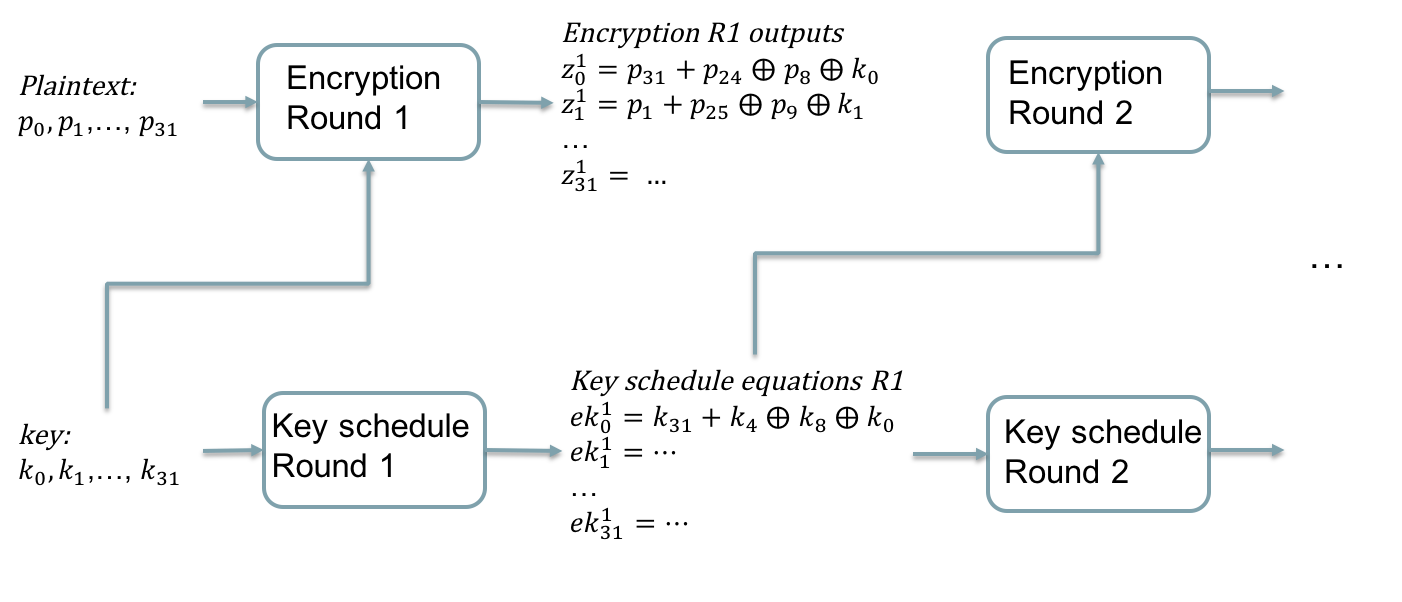
\includegraphics[width=130mm]{./pics/ch3ACmodeling.png}	
	\caption[Toy example for modelling Simon block cipher with a multivariate quadratic equation system]{Toy example for modelling Simon block cipher with a multivariate quadratic equation system. The upper part is the main block encryption with extended keys generated by a key schedule\protect\footnotemark (lower part). }
	\label{fig:ch3ACmodeling}
\end{figure}	
\footnotetext{The key schedule here has a specific recursive form %%%%found
	in popular ciphers such as DES, AES and Simon
	which optimizes storage or chip size and timing.}

% Algerbirc 
In addition, some high profile cryptanalysis problems in public key cryptography can be written in a form that contains a \textit{block cipher topology} \footnote{
	This is basically a property of the equations proposed by Semaev in 2015 \cite{semaev2004summation,cryptoeprint:2015:310}, they have  the same structure as on Figure \ref{fig:blockciphertopology} with variables progressively more and more remote from the constraints which make that the system of equations have a unique solution. The key point is that this sort of configuration leads to a system of equations which is really very hard to solve in the same way as in algebraic attacks on block ciphers.}. Such equations have a similar structure to a block cipher, where the beginning inputs and final outputs variables are easy to get and the middle part of the equation system is very hard to analyse (see Figure \ref{fig:blockciphertopology}). One example is Semaev's summation polynomial equations studied in elliptic curve cryptanalysis \cite{semaev2004summation,cryptoeprint:2015:310} see Section \ref{sec:SemaevCipher}.      

\begin{figure}[h!]
	\centering
	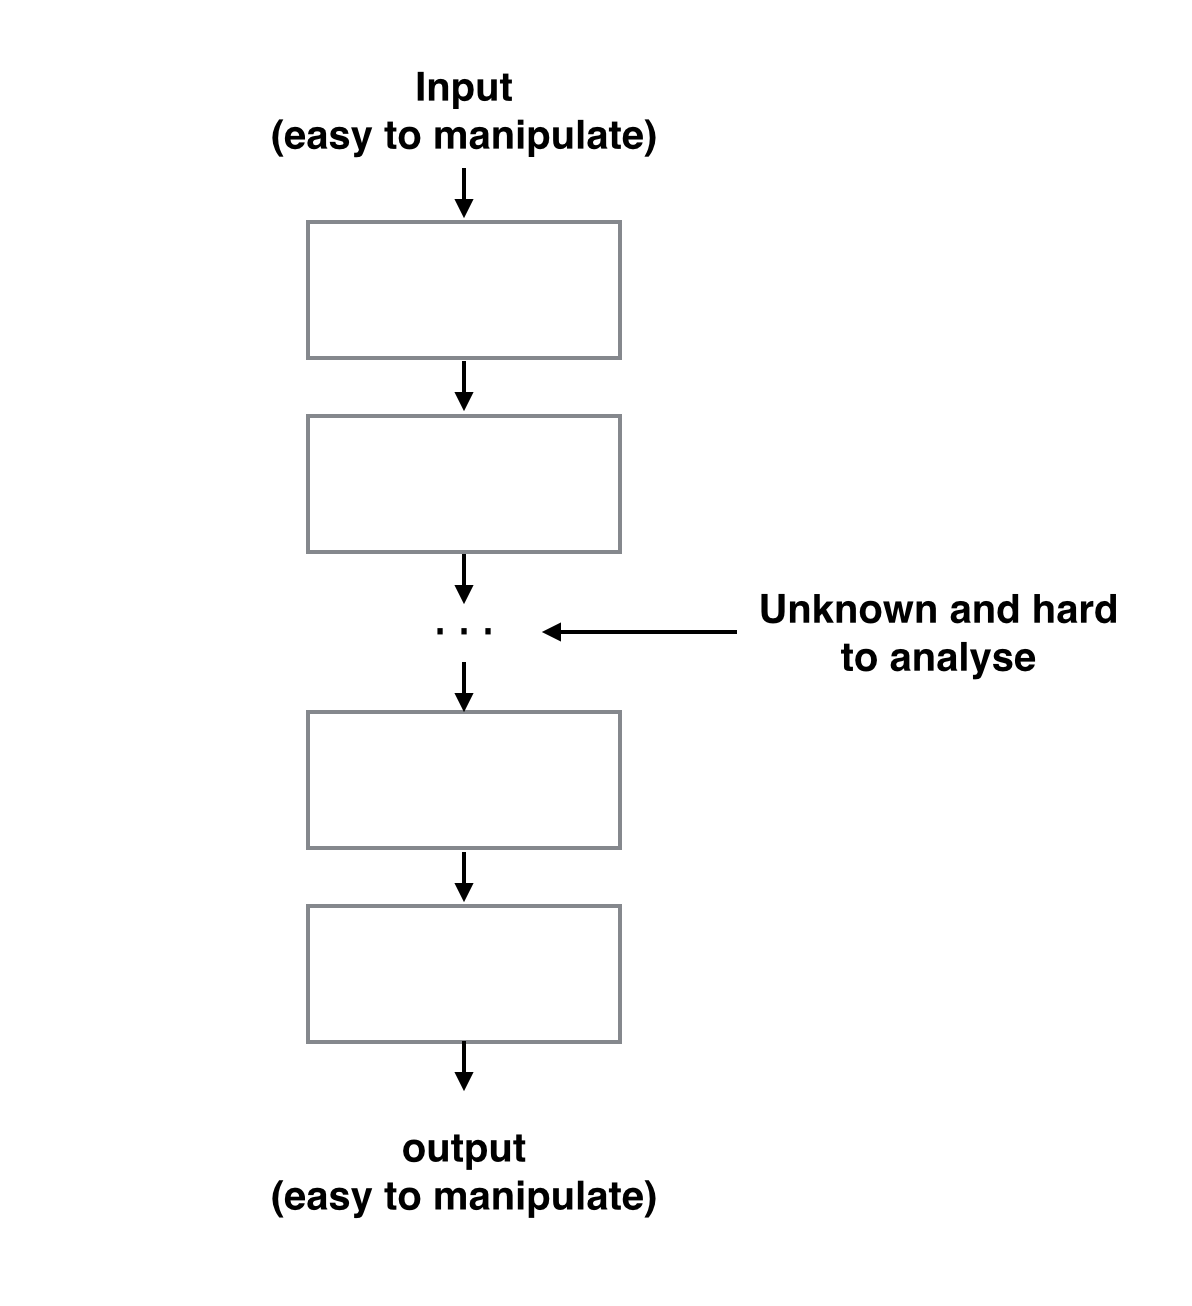
\includegraphics[width=130mm]{./pics/block_cipher_topology2.png}	
	\caption[Block cipher topology] {Block cipher topology: the attacker can control or manipulate
		the inputs and the outputs but it is quite hard to say anything about the variables in the middle}
	\label{fig:blockciphertopology}
\end{figure}	

\subsection{Algebraic Attacks Solving Stage}
Solving a random system of multivariate non-linear boolean equations is an NP-hard problem \cite{fraenkel1980complexity}. As many cryptographic primitives can be described by a sparse multivariate non-linear system of equations over $\mathbb{F}_2$ or any other algebraic systems, several techniques were developed to tackle the problem of solving these equations. A classic approach is to use techniques from algebraic geometry, especially Gr\"{o}bner bases algorithms, to solve the system of equations \cite{faugere1999new}. But most of the time they do not lead to solutions in practice due to the extremely high memory requirements. Subsequently, some heuristic techniques were developed called \textit{linearization} \cite{XL}, where all the non-linear terms are replaced by an independent linear variable and the resulting linear system can be solved using Gaussian elimination \cite{sepehrdad2012statistical}. However, this requires there to be enough linearly independent equations and that the initial system  be highly over-defined and sparse. Then, the XL algorithm \cite{XL,courtois2002cryptanalysis} was developed to make the system over-defined by adding new equations to the current system. The XL proposal made it possible to solve the multi-order non-linear equations within polynomial time, which accelerated the development of the algebraic attacks. Then researchers focused mainly on  fast solutions to the algebraic equation systems. 

Since 2006, Courtois and Bard discovered that this problem could be solved using tools and software \cite{courtois2007algebraicDES}, such as SAT solvers. SAT solvers are automated software solvers which aim to solve one of the original NP-complete problems, the so-called Boolean Satisfiability Problem. 
\begin{mydef} \label{def:booleanSat}[Boolean Satisfiability Problem] 
The SAT problem in Conjunctive Normal Form (CNF) consists of the conjunction ( $\wedge$  representing the Boolean AND connective) of a number of clauses, where a clause is a disjunction ( $\vee$ representing the Boolean OR connective) of a number of propositions or their negations (literals).

If $x_{i}$ represent propositions that can assume only the values True ($\equiv 1 \equiv \top$) or False ($\equiv 0 \equiv \bot$), then an example formula in CNF would be:
$$(x0 \vee x2 \vee x3) \wedge (x3) \wedge (x1 \vee \lnot x2)$$
where $\lnot x_{i}$ is the negation of $x_{i}$.
Given a set of clauses $C_{0}, C_{1}, ... , C_{m-1}$ on the propositions $x_{0}, x_{1}, ... , x_{n-1}$, the problem is to
determine whether the formula $$ F = \bigwedge_{j<m} C_{j}$$ has an assignment of truth values to the propositions such
that it evaluates to True.	
\end{mydef}
In the past decade, the rapid improvements in SAT algorithms has made SAT solvers increasingly popular. Modern SAT solvers have a significant impact on the fields of  electronic design automation, software verification, constraint solving in artificial intelligence, and operations research, among others.  Nicolas Courtois is the pioneer of bringing SAT solvers into action in the area of symmetric cryptanalysis. His paper \cite{bard2007efficient} described how to convert a multivariate quadratic equation system to CNF which can be solved automatically by SAT solvers. The advantage of this technique is that SAT solvers can perform reasonably well and do not require a lot of memory as compared with Gr$\ddot{o}$bner basis-based techniques \cite{grobner}. The only disadvantage is the unpredictability of its complexity. The first algebraic attack on reduced-round block cipher DES was done by Courtois and Bard in 2007 \cite{DEScourtois}. Later in 2008, the first algebraic attack on full block cipher KeeLoq \cite{courtois2008algebraicKeeLoq} took place. In the past 10 years, SAT solvers have been used for attacks on block ciphers, such as GOST \cite{courtois2012contradiction,gostac}, KATAN32 \cite{bard2010algebraic} and the Chinese block cipher SMS4 \cite{erickson2010algebraic},  stream ciphers, such as Crypto-1, HiTag2 and Bivium \cite{soos2009extending,courtois2009practical}, and MiFare Classic smart cards \cite{courtois2008algebraic}.

Another method is to use the ElimLin algorithm \cite{ElimLinR}. ElimLin stands for \textbf{Elim}inate \textbf{Lin}ear, and it is a simple algorithm for solving polynomial systems of multivariate equations over small finite fields. It was initially proposed as a single tool by Courtois to attack DES and CTC/CTC2 ciphers \cite{DEScourtois}. It is also known as the \textit{inter-reduction} step in all major algebra systems. Its main aim is to reveal some hidden linear equations existing in the ideal generated by the system of
polynomials. ElimLin is composed of two sequential stages:

\begin{itemize}
	\item \textbf{Gaussian Elimination:} To discover all the linear equations in the linear span of initial equations.
	\item \textbf{Substitution:} Variables are iteratively eliminated in the whole system based on the linear equations found until no linear equation is left.
\end{itemize}

Given an initial multivariate system of equations over $S^0$ in $\mathbb{F}_2[x_1,x_2,..,x_n]$, then the ElimLin is formally described in algorithm \ref{alg:ElimLin}.

\begin{algorithm} 
	
	\caption{ElimLin Algorithm}
	\begin{algorithmic}\label{alg:ElimLin}
		\STATE \textbf{Input:} $S^0=\{f_1,f_2,...,f_m\} \in \mathbb{F}_2[x_1,x_2,..,x_n]$
		\STATE \textbf{Output:} An updated system of equations $S^T$ and a system of linear equations $S_L$
		\STATE 1. Set $S_L\leftarrow{\O}$ and $S^T \leftarrow S^0$ and $k\leftarrow 1$
		\STATE 2. \textbf{Repeat}
		\STATE For some ordering of equations and monomials perform $Gauss(S^T)$ to eliminate non-linear monomials
		\STATE Set $S_{L'} \leftarrow$ Linear Equations from $Gauss(S^T)$
		\STATE Set $S^T\leftarrow Gauss(S^T)\backslash S_{L'}$
		\FOR {$\forall l \in S_{L'}$, $l$ non-trivial (if l=1and unsolvable then \emph{terminate})} 
		%\STATE Let $l \in S_{L'}$, $l$ non-trivial (if unsolvable then \emph{terminate})
		\STATE Let $x_{i_k}$ be a monomial in $l$
		\STATE Substitute $x_{i_k}$ in $S^T$ and $S_{L'}$ and replace by $l-x_{i_k}$
		\STATE Insert $l$ in $S_L$
		\ENDFOR
		\STATE $k\leftarrow k+1$
	\end{algorithmic}
\end{algorithm}

The study of ElimLin is interesting \cite{ElimLinRevisit,ElimLinUniversalEqs}
precisely because it is simpler to understand than more complex
polynomial algebra techniques \cite{XL,XL2,XLAsEstCourt04,Bardet,DoSemiRegularSequencesExist}. In recent years, ElimLin has been applied to NSA block cipher Simon, LBlock, KATAN32 and PRESENT \cite{courtois2014combined,RaddumSimon,ElimLinUniversalEqs,nakahara2009linear}. The main characteristic of ElimLin is that it quietly dissolves
and makes non-linear equations disappear and generates linear equations. Non-linearity is the main and only thing which makes cryptographic schemes not broken by simple linear algebra. Intuitively, ElimLin seems to work better in cases where there is low non-linearity, since this implies the existence of more linear equations.  Multiplicative complexity (MC) is another notion of non-linearity which was studied in Mourouzis's PhD thesis \cite{TheoPhD} and possibly Elimlin may work sufficiently well in cryptographic primitives with low MC.
However, the complexity of ElimLin attack or software algebraic attacks in general is not well studied. It is not clear why this works and how well the ElimLin attack scales for larger systems of equations. This is a major topic of interest in this thesis.

%

\subsection{Algebraic Complexity Reduction} \label{sec:ACReduction}

In order to break a full cipher, algebraic attacks are normally combined with other cryptanalysis techniques to reduce the solving complexity. This attack scenario consists of two independent tasks: one is how a reduced-round cipher can be solved by software algebraic cryptanalysis which we will discuss in Chapter \ref{ch:GOST}-\ref{ch:ElimLIn}. The other task is called algebraic complexity reduction \cite{gostreport,gostac}, which focuses on how the complexity of solving a full round cipher can be reduced to a problem of breaking a cipher with much fewer rounds. Algebraic complexity reduction raises an important optimization problem in algebraic cryptanalysis: one needs to minimize the costs (regarding the probability that our assumptions hold) and to maximize the benefits (regarding the number and the complexity of interesting relations
which hold under these assumptions).  Amplification which was introduced by Courtois and Debraize in 2008 \cite{AlgSnowCourtoisDebraize} is a notion which occurs in such optimization problems.

\begin{mydef}[Amplification, Informal]
	The goal of the attacker
	is to find a reduction where he makes some assumptions
	at a certain initial cost.
	For example they are true with probability $2^{-X}$
	or work for certain proportion $2^{-Z}$ of keys.
	Then the attacker can in constant time determine
	many other internal bits inside the cipher to the total of $Y$ bits.
	
	We are only interested in cases in which the values
	$X$ and $Z$ are judged realistically for a given attack,
	for example $Z<32$ and $X<128$.
	
	We call amplification the ratio $A=Y/X$.
\end{mydef}

The idea of amplification is to gain additional information inside the cipher with low cost. Amplification is also a general cryptanalysis principle which can apply to many cryptanalysis attacks. For example, a guess-then-determine process can be seen as a form of amplification. With the cost of guessing, attackers gain additional information about the key bits which might lead to knowledge about many other bits inside the cipher. 
Gordon Welchman's diagonal board is also a form of amplification which makes Turing's Bombe machine gain additional information about Enigma encryption settings \cite{CourtoisBlockEnigmaSlides}. 

%Algebraic complexity reduction can be very successful if the cipher has certain special properties. For example, in \cite{gostac}, Courtois found the Russian cipher GOST had many self-similarity properties, which reduced the problem of breaking the full GOST cipher from $2^{64}$ key pairs for 32 rounds to 4 key pairs for 8 rounds and similar results.

%Very little is known about what approach would make an algebraic attack efficient and why.

%phase transition and solving time for random 3 sat problems
%from hard to solve to easy to solve

\section{Cryptanlysis of GOST Block Cipher} \label{sec:introductionToGOST}
The Russian encryption standard
GOST 28147-89 %was developed in the 1970s
is an important government standard
\cite{gost198928147}.
Its large key size of 256 bits makes GOST a plausible alternative for AES-256 and 3-key triple DES.
%% full version maybe %%The latter for the same block size of 64 bits offers keys of only 168 bits.
This indicates that GOST means to be a serious cipher for serious applications
%% full version maybe %%designed with most serious applications in mind.
and at least two sets of GOST S-boxes have been explicitly identified as being used by the most prominent Russian banks, %financial institutions
cf. \cite{schneier2007applied,GOSTRussianReferenceImplementation}.

\subsection{GOST And ISO Standardisation.}
The cost of cryptography is still an important problem for the industry.
For example it was only around 2010 that Intel implemented an encryption algorithm
in some of its CPUs, and nowadays both Intel and AMD have very good support for AES-NI instructions.
It is therefore very important to notice that,
in addition to the very long bit keys,
GOST has a much lower implementation cost
than AES or any other comparable encryption algorithm.
For example, in hardware GOST 256 bits requires less than 800 GE\footnote{GE: (informally) 1 GE is equivalent to 1 AND gate },
while AES-128 requires 3100 GE \cite{PoschmannImplement}.
Thus it is not surprising that GOST became an Internet standard.
It is part of many crypto libraries such as OpenSSL
\cite{GOSTRussianReferenceImplementation}, %,Crypto++},
and is also increasingly popular %and used
outside its country of origin
\cite{PoschmannImplement}.
It is hard to think about a better algorithm for the industry
because of its ultra-low implementation cost and
20 years of cryptanalysis efforts behind it \cite{PoschmannImplement}.
In 2010 GOST was submitted to ISO 18033
to become a worldwide encryption standard.
Less than 10
%Only eight
block ciphers have ever become an
ISO %international
standard.
Unhappily in 2011 several key recovery attacks on GOST were found by researchers
\cite{JapaneseGOSTMITMFSE2011,gostreport,gostac,gostdc0,gostdc2}.

\subsection{Cryptanalysis of GOST} \label{sec:CrytanalysisGOST}
The turning point in the security of GOST was the discovery of the so called
``Reflection'' property described by Kara in Indocrypt 2008 \cite{GOSTReflectionKara}.

The reflection property in GOST is based on its key schedule. GOST is a Feistel cipher with 32 rounds. In each round we have a round function $f_k(X)$ with a 32-bit sub-key which is the original 256-bit key divided into eight 32-bit segments $k = (k_0, k_1, k_2, k_3, k_4, k_5, k_6, k_7)$.
One 32-bit sub-key is used in each round, and their exact order is shown in Table \ref{tab:GOSTKey}:

\begin{table}[!h]
	\centering
	\caption[Key Schedule in GOST]{Key schedule in GOST}
	\label{tab:GOSTKey}
	\addtolength{\tabcolsep}{-6pt}
	\resizebox{\textwidth}{!}{%
		\begin{tabular}{|c|c c c c c c c c|c c c c c c c c|c c c c c c c c|c c c c c c c c|}
			\hline
			rounds &1&&&&&&&8&9&&&&&&&16&17&&&&&&&24&25&&&&&&&32 \\ \hline
			keys & $k_0$ & $k_1$ & $k_2$ & $k_3$ & $k_4$ & $k_5$ & $k_6$ & $k_7$& $k_0$ & $k_1$ & $k_2$ & $k_3$ & $k_4$ & $k_5$ & $k_6$ & $k_7$&
			$k_0$ & $k_1$ & $k_2$ & $k_3$ & $k_4$ & $k_5$ & $k_6$ & $k_7$&
			$k_7$ & $k_6$ & $k_5$ & $k_4$ & $k_3$ & $k_2$ & $k_1$ & $k_0$  \\ \hline
			
	\end{tabular}}
\end{table}

Follow Kara's work in Indocrypt 2008 \cite{GOSTReflectionKara}, we write GOST as the following functional decomposition (to be read from right to left)
$$Enc_{k}=\mathfrak{D}  \circ S \circ \varepsilon \circ \varepsilon \circ \varepsilon$$
where $\varepsilon$ is the first 8 rounds which exploits the whole 256-bit key, $S$ is a swap function which exchanges the left and right hand sides and does not depend on the key, and $\mathfrak{D}$ is the corresponding decryption function with $\varepsilon \circ \mathfrak{D}  = \mathfrak{D} \circ \varepsilon = Id$.

Initially at Indocrypt 2008 only a weak-key attack with time complexity of $2^{192}$ was proposed, with a large proportion of $2^{-32}$ of weak keys. Then in 2011, Courtois propsed an algebraic complex reduction attack which break full 32 rounds GOST using pure algebraic cryptanalysis. 

\begin{myAssumption} \label{AssumptionW}
	\cite{gostreport} Let $A$ be such that $\varepsilon(D) = \overline{D}$ where $D$ is defined as $D=\varepsilon^{3}(A)$.
\end{myAssumption}

\begin{fact}
	\cite{gostreport} Given $2^{64}$ known plaintext there is on average one value $A$ which satisfies Assumption \ref{AssumptionW}. For 63\% of all GOST keys at least one such $A$ exists.
\end{fact}

\begin{fact} 
\cite{gostreport} If $A$ satisfies the Assumption \ref{AssumptionW} and defining $B = \varepsilon(A) $ and $C = \varepsilon(B)$ we have:
\begin{enumerate}
	\item $Enc_k(A) = D$. This is illustrated on the right hand side of Figure \ref{GOSTRef}
	\item $Enc_k(B) = C$. This can be seen on the left hand side of Figure \ref{GOSTRef}
\end{enumerate}
\end{fact}

\begin{figure}[h!] 
	\centering
	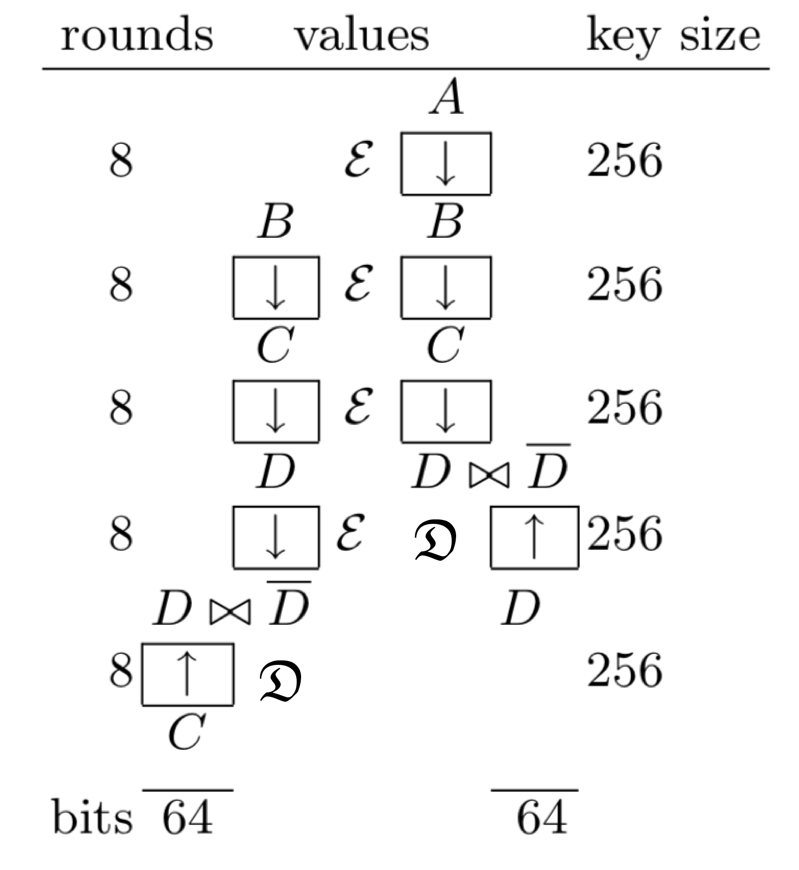
\includegraphics[width=80mm]{./pics/GOSTRef.png}
	
	\caption[Algebraic Complexity Reduction from 32 to 8 rounds of GOST] {Algebraic Complexity Reduction from 32 to 8 rounds of GOST. Due to GOST's self similiarity in the key schedule, the problem of breaking full 32 rounds can be reduced to 8 rounds. The idea is to find 2 Known Plaintext $A$ and $B$ that has properties shown in this figure. }
	\label{GOSTRef}
\end{figure}

\paragraph{From $2^{64}$ KP for 32 Rounds to 4 KP for 8 Rounds:}
Given $2^{64}$ known plaintexts for GOST, it is possible to obtain 4 P/C pairs for 8 rounds of GOST and our guess will be correct with probability $2^{128}$. Thus we obtained 4 pairs for 8 rounds of GOST: $A 􏰀\rightarrow B, B \rightarrow C, C \rightarrow D, D \rightarrow \overline{D}$. As a result breaking 4 P/C pairs 8 rounds of GOST become the last step of breaking full GOST. Courtois said in his papaer the time complexity of breaking 8 rounds GOST is $2^{120}$ \cite{gostreport}. In this thesis we look precisely at questions pertaining to cryptanalysing 8 rounds GOST with less or equal than 4 P/C pairs which can be used as a plugin to replace already known attacks on full GOST.

Many attacks which do not use any reflections
have also been proposed \cite{gostac,gostreport,DunkelmanImprovedGOST8R}
and also differential attacks which do not
fall into the algebraic complexity reduction category.
The most recent advanced differential attack on GOST
has a time complexity of $2^{178}$ \cite{gostdc0,gostdc2}
which is also the best single-key attack known.

\subsection{The Internal Structure of GOST} \label{sec:GOSTStructure}
GOST is a block cipher with a simple Feistel structure,
64-bit block size, 256-bit keys and 32 rounds.
Each round contains a key addition modulo $2^{32}$,
a set of 8 bijective S-boxes on 4 bits,
and a simple rotation by 11 positions.

GOST has 32 identical rounds such as the one described on Figure \ref{GostRoundAndConnections} below.
They differ only by the subsets of 32 key bits which they use. GOST has a weak key schedule which is the main source of all the attacks on full 32-round GOST \cite{gostreport,gostac,JapaneseGOSTMITMFSE2011,gostdcpp1,gostdc0,gostdc1,gostdc2,DunkelmanImprovedGOST8R}.  
In this thesis we only look at up to 8 rounds of GOST which have independent 32-bit keys and don't repeat.

We number the inputs of the S-box Si for $i=1,2,\ldots,8$ by integers from $4i+1$ to $4i+4$ out of $1..32$ and its outputs are numbered according to their final positions after the rotation by 11 positions: for example the inputs of S6 are $21,22,23,24$ and the outputs are $32,1,2,3$.


\begin{figure}[h] 
	\centering
	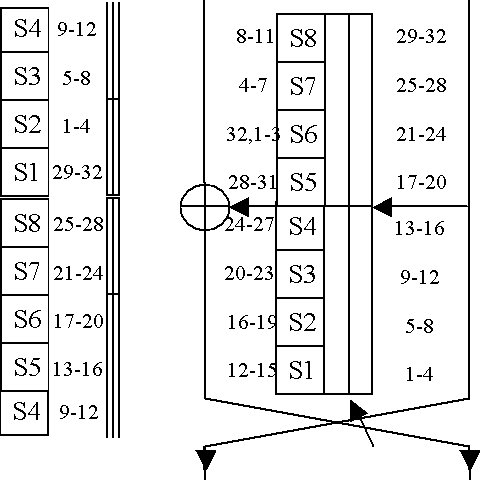
\includegraphics[width=80mm]{./pics/gostfeist2.jpg}
	
	\caption[One Round of GOST And Connections in The Following Round] {One Round of GOST And Connections in The Following Round. This figure describes the encryption process for one round of GOST. Firstly, the 32-bit right half is added with $k_{i}$ (modulo $2^{32}$, showed in figure as  $\boxplus$ ). Then, the result is divided into eight 4-bit consecutive blocks and each block is given as input to a different S-box. The first 4 bits go into the first S-box S1, bits 5-8 go into S2 and so on. Then, the 32-bit output undergoes a 11-bit left circular shift and finally the result is xored to the left 32-bit half of the data.}
	\label{GostRoundAndConnections}
\end{figure}

In Figure \ref{GostRoundAndConnections}
we also show S-box numbers
in the next round in the left margin.
This is very helpful in order to see which bits are successfully determined in our attacks on GOST.
In a great simplification, in most cases, one S-box in one round affects essentially
only two consecutive S-boxes in the next round. Additional propagation is obtained due to the Feistel structure
and due to carries in the modular addition.

\textbf{Modular Addition}: The GOST cipher uses addition modulo $2^{32}$ for key insertion which is another source of introducing non-linearity in the cipher. Here we explain how to algebraically encode modular addition, which is the modelling step of algebraic cryptanalysis. The modular addition of two n-bit words x; y is algebraically
described as follows
\begin{equation}
	(x,y) \mapsto z = x + y \text{ mod } 2^{n}
\end{equation}
The resulting n-bit word $(z_{n-1},...,z_{0})$ is given by:
\[
\left\{
\begin{array}{ll}
z_0 = x_0+y_0\\
z_1 = x_1+y_1+c_1\\
z_2 = x_2+y_2+c_2\\
.\\
z_i=x_i+y_i+c_i \\
.\\
z_{n-1} = x_{n-1} + y_{n-1}+c_{n-1}
\end{array}
\right.
\]
where,
\[
\left\{
\begin{array}{ll}
c_1 = x_0  y_0\\
c_2 = x_1 y_1+c_1(x_1+y_1)\\
.\\
c_i=x_{i-1}y_{i-1}+c_{i-1}(x_{i-1}+y_{i-1})\\
.\\
c_{n-1} = x_{n-2}+y_{n-2}+c_{n-2}(x_{n-2}+y_{n-2}) 
\end{array}
\right.
\]

\section{Cryptanalysis of SIMON Block Cipher}
Nowadays lightweight cryptography is rapidly evolving and becoming more and more important due to the increasing demand from mobile phones and the Internet of Things. These lightweight cryptographic primitives are designed to
be efficient (in both hardware and software) when limited
hardware resources are available and at the same time to
guarantee a desired level of security. The
design of such primitives is a great challenge and can be
seen as a non-trivial optimization problem, where several
trade-offs are taken into account. They need to maintain
a reasonable balance between security and efficient software and hardware
implementation with very low overall cost with respect to several
meaningful metrics (power consumption, energy consumption, size of the circuit \cite{OptimiPaper,BoyarPeraltaMCMethod,BoyarPeraltaMCBoolean}).

The research community has
proposed many lightweight hash functions, block ciphers and stream ciphers which are
reasonably good and satisfy at a reasonable level the trade-off
between efficiency and security. Nowadays, in cryptographic
literature we find lots of such lightweight cryptographic primitives such as
KATAN \cite{KATAN}, KLEIN \cite{KLEIN}, ICEBERG
\cite{ICEBERG}, HIGHT \cite{HIGHT}, LED \cite{LED},
mCrypton \cite{mCrypton}, PRESENT \cite{PRESENT}, Piccolo \cite{Piccolo}
and many others.

In July 2013, a team from the NSA proposed two new families of particularly lightweight block
ciphers, Simon and Speck, both coming in a variety of blocks and key sizes
\cite{NSAciphers}. We have developed a basic reference implementation of both ciphers 
which can be found on Github \cite{simonref},
as well as a generator of algebraic equations to be used in algebraic attacks. 

The designers of Simon and Speck published the full specifications and presented
only performance and implementation footprints, without providing
any advanced security analysis
against known cryptanalytic attacks.
Both of them offer excellent performance on both
hardware and software platforms and perform
exceptionally well across the majority of lightweight applications and
not only on a single platform. Compared to
other lightweight cryptographic primitives,
these two are meant to have better performance with respect to the area
needed for a given throughput, code size and memory usage.
Simon is designed for optimal performance in hardware, and Speck for optimal
performance in software.
According to Aysu's analysis \cite{simoneff}, Simon with an equivalent security level as AES,
is $86\%$ smaller
than AES, $70\%$ smaller than PRESENT and its smallest hardware architecture
only costs 36 slices (72 look-up tables, 30 registers). Recent results about hardware
implementation of block ciphers emphasize reducing the size and/or Multiplicative Complexity (MC) further possibly
leads to optimal implementations \cite{BoyarPeraltaMCMethodAES,OptimiPaper}.

However, in the original NSA paper \cite{NSAciphers}, there is no analysis of the security of these 2 ciphers against major well-known attacks. In the same paper \cite{NSAciphers}, the authors briefly said that Simon and Speck were designed to provide security against traditional adversaries who can adaptively encrypt and decrypt large amounts of data, and some attention was given so that there are no related-key attacks. Except for these comments, no more analysis against common attacks such as linear or differential cryptanalysis was presented and the task of analyzing the resistance of the ciphers against known attacks was left to the academic community. Immediately after the release of the specifications we had the first attempts using differential, linear and rotational cryptanalysis \cite{simon1,simon2}. Our attacks on Simon described in Chapter \ref{ch:SIMON} were the first algebraic cryptanalysis attacks attempted on Simon. The work was published in 2014 \cite{courtois2014combined}. In recent years Simon was studied heavily by a lot of researchers, including differential attacks introduced by Biryukov et al \cite{simon3}, Mourouzis et al \cite{SIMON6} and Wang et al \cite{SIMON4, SIMON5}, also combined differential and linear attacks by Farzaneh et al \cite{simon1} and Alkhzaimi et al \cite{simon2}. Most of them are using statistical cryptanalysis techniques, the best results break around 70\% rounds of different versions of Simon. In 2015, Raddum \cite{raddum2006new} published another algebraic cryptanalysis work on Simon for most of the versions (not including Simon 64/128 version). Raddum's work uses more P/C pairs than our attack and breaks 16 (out of 72) rounds of Simon 128/256 version with ElimLin.  This attack shows that there is a need to understand better how ElimLin attacks can scale to larger attacks. 

\subsection{SIMON Structure}
SIMON is a family of lightweight block ciphers with the aim of havingan  optimal hardware performance \cite{NSAciphers}.
It follows the classical Feistel design paradigm\footnote{Note that in classical Feistel structure computation is done on left side, see \ref{sec:feistel}. In Simon computation is done on right side see Figure \ref{fig:SIMONroundfn}}, operating on two
$n$-bit halves in each round and thus the general block size is $2n$.
The Simon block cipher with an $n$-bit word is denoted by Simon-$2n$, where
$n=16,24,32,48$ or $64$, and if it uses an $m$-word key (equivalently $mn$-bit
key) we denote it as Simon-$2n/mn$. In this chapter, we study the variant of
Simon with $n=32$ and $m=4$ (i.e. 128-bit key).

Each round of Simon applies a non-linear, non-bijective (and as a result
non-invertible) function
\begin{equation}
F:GF(2)^n\rightarrow GF(2)^n
\end{equation}

to the left half of the state which is repeated for 44 rounds.
The operations used are as follows:

\begin{enumerate}
	\item bitwise XOR, $\oplus$
	\item bitwise AND,
	\item left circular shift, $S^j$ by $j$ bits.
\end{enumerate}

We denote the input to the $i$-th round by $L^{i-1}||R^{i-1}$
and in each round the left word $L^{i-1}$ is used as input
to the round function $F$ defined by,

\begin{equation}
F(L^{i-1})=(L^{i-1}<<<1)\wedge(L^{i-1}<<<8)\oplus(L^{i-1}<<<2)
\end{equation}

Then, the next state $L^{i}||R^{i}$ is computed as follows
(cf. Fig. \ref{fig:SIMONroundfn}),

\begin{equation}
L^i=R^{i-1}\oplus F(L^{i-1})\oplus K^{i-1}
\end{equation}
\begin{equation}
R^i=L^{i-1}
\end{equation}


\begin{figure}[!h]
	\vspace{-0.2cm}
	\centering
	%   {\epsfig{file = .\SIMONroundfn.eps, width = 6.5cm}}
	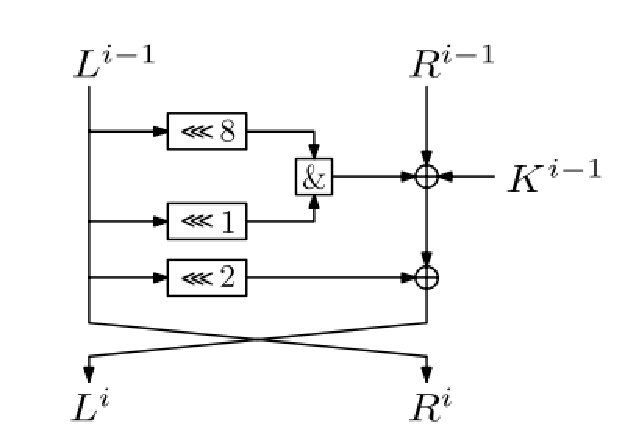
\includegraphics[width=120mm]{./pics/SIMONroundfn-eps-converted-to.pdf}
	\caption{The round function of Simon}
	\label{fig:SIMONroundfn}
	\vspace{-0.1cm}
\end{figure}


The output of the last round is the ciphertext.
\subsection{Key Schedule}
The key schedule of Simon is based on an Linear-Feedback Shift Register(LSFR)-like procedure \cite{lindell2014introduction}, where the $nm$-bits of the key are used to generate the keys $K_0,K_1,...,K_{r-1}$ to be used in each round. There are three different key schedule procedures depending on the number of words that the secret key consists of ($m=2,3,4$).

At the beginning, the first $m$ words $K^0,K^1,...,K^{m-1}$ are initialized with the secret key, while the remaining are generated by the LSFR-like construction. For the variant of  interest, where $m=4$, the remaining keys are generated in the following way:
\begin{equation}
Y=K^{i+1}\oplus (K^{i+3}>>>3)
\end{equation}
\begin{equation}
K^{i+4}=K^i\oplus Y \oplus (Y>>>1)\oplus c\oplus (z_j)_i
\end{equation}

The constant $c=0xff...fc$ is used for preventing slide attacks and attacks exploiting rotational symmetries \cite{NSAciphers}. In addition, the generated subkeys are XORed with a bit $(z_j)_i$, that denotes the $i$-th bit from the one of the five constant sequences $z_0,...,z_4$. These sequences are defined in the NSA's orginial paper \cite{NSAciphers} and for our variant we use $z_3$. We have implemented a basic reference implementation of Simon and Speck ciphers and a basic generator of equations that are used in algebraic attacks \cite{simonref} .

The Feistel network, the construction of the round function and the key generation of Simon, enables bit-serial hardware architectures which can significantly reduce the cost of implementation \cite{simoneff}. Additionally, encryption and decryption can be done using the
same hardware.

\section{Summary} \label{sec:ACCxty}
Algebraic cryptanalysis attacks allow the cryptanalyst to recover secret key bits given only one or very few plaintext / ciphertext pairs. However, one of the fundamental problems of algebraic cryptanalysis is that the runtime of algebraic attacks against block ciphers is not well understood. In 2007, Courtois and Bard said in the first paper describing an algebraic attack on block cipher \cite{DEScourtois}:

\begin{quotation}
	``Very little is known about what approach would make an algebraic attack efficient and why." 
\end{quotation}


Up to today, this question still remains in algebraic cryptanalysis. At the moment most of the exising Algebraic Cryptanalysis applications are just coverting target ciphers to equation systems and then solved directly by a software solver  (i.e ElimLin or SAT solvers). Very limited research has been done in order to understand the behavior of a solver and how to make the coverted equation system become easier to solve. 

On cryptanalysis of block ciphers we introduced two well known encryption standards: Russian GOST and NSA SIMON. We reviewed the state of art cryptanalysis works on these encryption standards: best algebraic cryptanalysis attack on 8 rounds GOST require time complexity of $2^{120}$ and no algebraic cryptanalysis has been done on SIMON. The above facts motivate our research work decribed in Part \ref{Part2} of the thesis. 

In Chapter \ref{ch:GOST} we will introduce a fundemental notion of ``contradiction immunity`` and describe how conradiction can be used in algebraic cryptanalysis. We will demostrate a mixed SAT/UNSAT attack on GOST which improve the time complexity of current best attack on breaking 8 rounds of GOST from $2^{120}$ to $2^{92}$. In Chapter \ref{ch:SIMON} we will describe a new Algebraic Cryptanalysis approach combined with well selected P/C paris in a Chosen Plaintext Attack scenario and benchmark our attacks with randomly selected P/C pairs. We will apply this method in newly proposed NSA cipher SIMON and provide the first Algebraic Cryptanalysis on SIMON block cipher. Finally in Chapter \ref{ch:ElimLIn} we will study the behavior of ElimLin method with regards to the number of data samples availiable to an attacker. By studying the number of linear independent equations found by ElimLin, we will show ElimLin has a phase transition process where the number of equations found by ElimLin increase much faster than linear and eventually break the cipher. We will then inspect where the faster than linear groth come from and study how to find more equations that ElimLin can not yet find.


\chapter{Introduction to Elliptic Curves} \label{Ch:EllipticCurve}
\section{Mathematical Foundations}
\subsection*{Finite Groups}
A Finite Group is a set G with a finite number of $q$ elements, which has a binary operation $*$ : $G * G \rightarrow G$ and satisfies the following properties \cite{hankerson2006guide}:
\begin{enumerate}
	\item Associativity: $(a*b)*c=a*(b*c)$ for all elements $a,b,c \in G$
	\item Existence of an identity: there exists an element $e \in G$ such that $a*e=e*a=a$ for all $a \in G$. Element $e$ is called the neutral element (or identity element) of the group.
	\item Existence of inverses: for each element $a \in G$, there exists an element $b \in G$ such that $a*b=b*a=e$. Element $b$ is called the inverse of $a$.
\end{enumerate}
$q$ is called the group order. In addition, a group is called Abelian group (or commutative group) if it satisfies the commutativity law which is $a*b=b*a$ for all elements $a,b \in G$. 

If the binary operation is called addition (+), then the group is additive. In this case, the neutral element is usually denoted by 0 and the additive inverse of an element $a$ is denoted by $-a$. If the binary operation is called multiplication $(\cdot)$, then the finite group is multiplicative. In this case, the identity element is usually denoted by 1 and the multiplicative inverse of an element $a$ is denoted by $a^{-1}$.

\subsection*{Finite Fields}
Abstractly, a finite field consists of a finite set of objects called field elements together with the description of two operations, addition and multiplication, that can be performed on pairs of field elements. These operations must have certain properties: \cite{hankerson2006guide}
\begin{enumerate}
	\item $(\mathbb{F},+)$ is an Abelian group with (additive) neutral element denoted by 0.
	\item $(\mathbb{F},\cdot)$ is an Abelian group with (multiplicative) neutral element denoted by 1.
	\item The distributive law holds: $(a+b) \cdot c = a \cdot c + b \cdot c$ for all $a,b,c \in \mathbb{F}$. 
\end{enumerate}

\paragraph{Prime Fields}\mbox{}\\
Let $p$ be a prime number. The residues modulo $p$, consisting of the integers $\left\lbrace 0,1,2,\dots,p-1\right\rbrace $ with addition and multiplication performed modulo $p$, is a finite field of order $p$.
\paragraph{Binary Fields}\mbox{}\\
Finite fields of order $2^m$ are called binary fields or characteristic-two finite fields. One way to construct $\mathbb{F}_{2^m}$ is to use a polynomial basis representation. The elements of $\mathbb{F}_{2^m}$ are the binary polynomials (polynomials whose coefficients are in the field $\mathbb{F}_2=\{0,1\}$) of degree at most $m-1$:
$$\mathbb{F}_{2^m}=\left\lbrace a_{m-1}z^{m-1}+\dots+a_2z^2+a_1z^1+a_0 : a_i \in \mathbb{F}_2 ;+, \cdot \right\rbrace. $$
An irreducible binary polynomial $f(z)$ of degree m is chosen. Irreducibility of $f(z)$ means that $f(z)$ cannot be factored as a product of binary polynomials each of degree less than $m$. Addition of field elements is the usual addition of polynomials, with coefficient reduced modulo 2. Multiplication of field elements is performed as multiplication of polynomials modulo the polynomial $f(z)$. 
\subsection*{Cyclic Groups}
Let $G$ be a finite group of order $q$ with multiplication ($\cdot$) as binary operation, $g$ be a group element of $G$, then the order of $g$ is the smallest positive integer $r$ for which $g^r = 1$.  
$G$ is called cyclic if there exist a $g$ such that $\langle g \rangle = \left\lbrace g^i : 0 \leq i \leq r-1 \right\rbrace $ is the subgroup of $G$ generated by $g$. If $r=q$ then $G$ is a cyclic group with generator $g$ if $G = \langle g \rangle$. The set $\langle
 g \rangle$ is also a group itself under the same binary operation and is called the cyclic subgroup of $G$ generated by $g$.
 
%\subsection{Generalized discrete logarithm problem}
%Given a multiplicative cyclic group $(G,\cdot)$ of order n with generator g and an element $y \in \

\section{Elliptic Curves} \label{sec:EC}
An elliptic curve over a field $K$ is defined by a set of points which satisfy the following equation (also known as standard Weierstrass form) and a group operation which will be defined later.
\begin{equation} \label{eq:ECWeierstrass}
y^3+a_1xy+a_3y = x^3 + a_2x^2+a_4x+a_6
\end{equation}

Here: $a_1,a_2,a_3,a_4,a_6 \in K$, and the discriminant is defined as
 $$\Delta=-d^{2}_{2}d_{8}-8d_{4}^{3}-27d_{6}^{2}+9d_{2}d_{4}d_{6} \neq 0$$
where  
$$d_{2}=a_{1}^{2}+4a_{2}$$  $$d_{4}=2a_{4}+a_1a_3$$  $$d_6=a_{3}^{2}+4a_6$$  $$d_8=a_{1}^{2}a_6+4a_2a_6-a_1a_3a_4+a_2a_{3}^{2}-a_{4}^{2}$$

The condition $\Delta \neq 0$ guarantees that there does not exist more than one tangent line for a given point on the curve.

For an elliptic curve over a field K of characteristic $\neq$ 2 or 3, without loss of generality, one can assume that $a_1=a_2=a_3=0$, we have $d_2=0$, $d_4=2a_4$, $d_6 = 4a_6$ and $d_8=-a_{4}^{2}$ \cite{hankerson2006guide}. Accordingly, the condition $\Delta = -16(4a_4^3+27a_6^2) \neq 0$ can be simplified to $4a_4^3+27a_6^2 \neq 0$. Consequently in practical application of elliptic curves, the curve equation is written in the following form:

\begin{equation} \label{eq:ECFp}
y^3=x^3+ax+b
\end{equation}

where $a=a_4$ and $b=a_6$, cf. Equation \ref{eq:ECWeierstrass}.

For an elliptic curve over binary fields $\mathbb{F}_2^m$, without loss of generality, one can assume that $a_1=1$, $a_3=a_4=0$ \cite{hankerson2006guide}. Then we have $d_2=1$, $d_4=0$, $d_6=0$ and $d_8=a_6$ \footnote{In binary fields anything multiplied by 2 equals to 0.}, and $\Delta = -a_6 \neq 0$. The short form of curve equation is normally written as follows: 
\begin{equation}\label{eq:ECF2m}
y^2+xy=x^3+ax^2+b
\end{equation}

where $ a = a_2$ and $b = a_6$ and $a,b \in \mathbb{F}_2^m$. 
%\cite{koblitz1987elliptic}

\subsection{Elliptic Curves Over $\mathbb{F}_p$}
The finite field $\mathbb{F}_p$ uses the numbers from 0 to $p-1$, and computations are done modulo $p$. An Elliptic Curve over finite field $\mathbb{F}_p$ where $p$ is a large prime, can be formed by choosing the constants $a$ and $b$ within the field $\mathbb{F}_p$. The elliptic curve includes all points $(x,y)$ which satisfy the elliptic curve equation modulo $p$ (where x and y are numbers in $\mathbb{F}_p$). It is typically defined in the short Weierstrass form:
$$y^2 \text{ mod } p= x^3 + ax + b \text{ mod } p$$

where $a,b \in \mathbb{F}_p$ satisfy $4a^3 + 27b^2 \text{ mod }p$ is not 0, which guarantees $x^3 + ax + b$ contains no repeated factors and then the elliptic curve is a group. The elliptic curve contains all points $P = (x,y)$ for $x,y \in F_p$ that satisfy the elliptic curve equation with addition of (for Weierstrass curves) a special point $\mathcal{O}$ called the point at infinity \footnote{In code implementation, $\mathcal{O}$ is normally be represented as point (0,0), but not always, as (0,0) might satisfy the curve equation.}.   
    
To give an example, consider an elliptic curve over the field $F_{19}$, where $a=1$ and $b=6$, the curve equation is: $y^2 = x^3 + x + 6$, an example used in \cite{balasubramanian1998improbability}. There are 18 points: 
\begin{center}
 $ (0,5)$, $(4,6)$, $(2,4)$, $(3,6)$, $(14,3)$, $(12,13)$, \\
$ (18,2)$, $(10,3)$, $(6,0)$, $(10,16)$, $(18,17)$, $(12,16)$, \\
$ (14,16)$, $(3,13)$, $(2,15)$, $(4,13)$, $(0,14)$, $\mathcal{O}$ 
\end{center}
The point $P=(4,6)$ satisfies this equation since:
\begin{center}
$ 6^2 \mod{19} = 4^3 + 4 + 6 \mod{19} $\\
$ 17 = 17 $ 
\end{center}
\textbf{Remark:} In mod $p$ Weierstrass curves $-(x,y) = (x,-y)$

\subsection{Binary Elliptic Curves}
Elements of the field $\mathbb{F}_{2^m}$ are m-bit strings. The rules for arithmetic in binary field can be defined by either polynomial basis or by so-called (more efficient) [optimal] normal basis\cite{IEEEP1363}. An elliptic curve $E$ with the underlying field $\mathbb{F}_{2^m}$ is given through the following equation: $$y^2+xy=x^3+ax^2+b$$ where $x,y,a,b \in \mathbb{F}_{2^m}$ and $b \neq 0$. The elliptic curve $E$ includes all points $(x,y)$ which satisfy the curve equation over $\mathbb{F}_{2^m}$, together with a point at infinity $\mathcal{O}$. 

To given an example, assume the finite field $\mathbb{F}_{2^4}$ has irreducible polynomial $f(x)=x^4+x+1$ (or $\mathtt{0x13}$ in hex). The element $g = (0010)$ is a generator for the field. The powers of g are:
%{small eq1 eq2}
\begin{small}
$$g^0=(0001), g^1=(0010), g^2=(0100), g^3=(1000), g^4=(0011),g^5=(0110)$$
$$g^6=(1100), g^7=(1011), g^8=(0101), g^9=(1010), g^{10}=(0111),g^{11}=(1110)$$
$$g^{12}=(1111), g^{13}=(1101), g^{14}=(1001), g^{15}=(0001)$$
\end{small}
%put somewher I have developed a lab for UCL  in which student can benchmark field operations, SCA etc 
%low level c/c++ programming
Consider the elliptic curve $y^2+xy=x^3+g^4x^2+1$. The points on $E$ are the following and shown in Figure \ref{fig:ecc_gf2m_example}.
\begin{small}
$$(1,g^{13}), (g^3,g^{13}) ,(g^5,g^{11}),(g^6,g^{14}),(g^9,g^{13}),(g^{10},g^8),(g^{12},g^{12}),$$
$$(1,g^6),(g^3,g^8),(g^5,g^3),(g^6,g^8),(g^9,g^{10}),(g^{10},g),(g^{12},0),(0,1), \mathcal{O}$$
\end{small}
    \begin{figure}[h!]
    	\centering
    	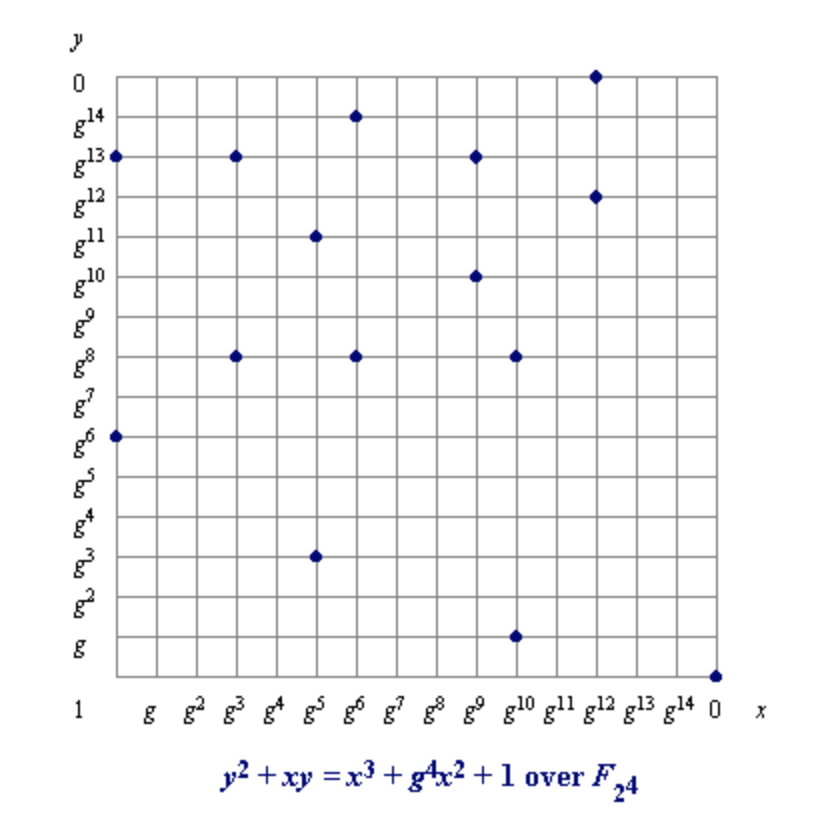
\includegraphics[width=100mm]{./pics/example_of_gf2m.png}
    	\caption{Example of elliptic curve over $\mathbb{F}_{2^4}$ }
    	\label{fig:ecc_gf2m_example}
    \end{figure}
    
\section{Point Arithmetic}
\subsection*{Point Addition for Prime Curves}
Let $P$ and $Q$ be two distinct points on an elliptic curve, and $P$ not equals to $-Q$. To add the points $P$ and $Q$, a line \footnote{line is a set of points which satisfy the equation $Ax+By+C = 0$ where $A,B,C \in \mathbb{F}_p$} is drawn through the two points. This line will have exactly one additional intersection point with the elliptic curve, which we call $-R$. The point $-R$ is ``reflected" in the x-axis to obtain point $R$. The law for point addition in an elliptic curve group is $P+Q=R$.  An example of geometrical graph is given in Figure \ref{fig:ecc_point_addition}. 
    \begin{figure}[h!]
    	\centering
    	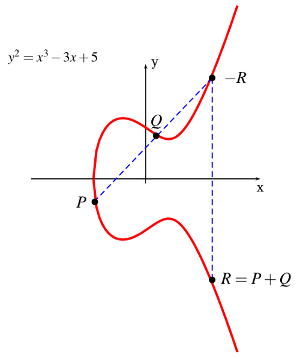
\includegraphics[width=65mm]{./pics/ecc_point_addition.png}
    	\caption{Elliptic curve point addition}
    	\label{fig:ecc_point_addition}
    \end{figure}
    
For point addition of $P$ and $-P$, the line through $P$ and $-P$ is a vertical line which does not intersect the elliptic curve at a third point. Thus the point $P$ and $-P$ cannot be added using the above method. In this case we define $P + (-P) = \mathcal{O}$. 

\subsection*{Point Doubling for Prime Curves}
Adding a point $P(x,y)$ to itself, a so-called tangent line to the curve is drawn at point $P$. If y is not zero, then the tangent line has exact one intersection with the curve at point $-Q$. $-Q$ is reflected in the x-axis to point $Q$. This operation is called doubling the point $P$, and the law for doubling is the following (also shown in Figure \ref{fig:ecc_point_doubling}): 
$$P+P=2P=Q$$ 

    \begin{figure}[h!]
    	\centering
    	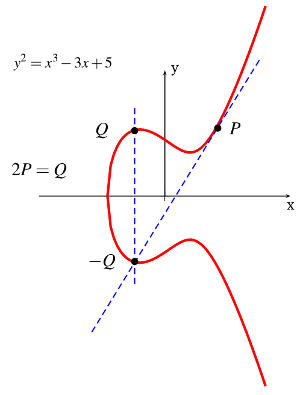
\includegraphics[width=65mm]{./pics/ecc_point_doubling.png}
    	\caption{Elliptic curve point doubling}
    	\label{fig:ecc_point_doubling}
    \end{figure}
    
Doubling the point $P(x,y)$ while $ y=0 $ then the tangent line to the curve is vertical and does not intersect the curve on any other point. For such a $P$, by definition, $2P=\mathcal{O}$, and $3P$ in this case, is $2P+P = \mathcal{O} + P = P$.   

\subsection*{Explicit Formulas for Prime Curves} \label{sec:affine_formulas}
For elliptic curves over $\mathbb{F}_p$, consider two points $P=(x_1,y_1)$ and $Q=(x_2,y_2)$, $P \neq \pm Q$, the point $P+Q = (x_3,y_3)$ is given by:
$$\lambda = \frac{y_2-y_1}{x_2-x_1}$$
$$x_3=\lambda^2-x_1-x_2$$
$$y_3=\lambda(x_1-x_3)-y_1$$

When $P=-Q$, $P+Q$ equals point at infinity $\mathcal{O}$. When $P=Q$, we apply the doubling formula:
$$\lambda = \frac{3x_1^2+a}{2y_1}$$
$$x_3=\lambda^2-2x_1$$
$$y_3=\lambda(x_1-x_3)-y_1$$



\subsection*{Scalar Multiplication}
Given an elliptic curve $E$ defined over a finite field $\mathbb{F}_p$, if $P \in E$ is a point of order $r$, the cyclic subgroup of $E$ generated by $P$ is ${\mathcal{O},P,2P,\ldots,(r-1)P}$. Then if we define the scalar $k$ as an integer within the range $[1,r-1]$, we can multiply a point by the scalar $k$ and we obtain: $Q=kP$, where $Q$ is also a point which belongs to the subgroup generated by $P$. 

\section{ECDLP}
The hardness of cryptosystem using elliptic curve point multiplication is based on the Elliptic Curve Discrete Logarithm Problem, which is an adaptation of traditional discrete logarithm problem to elliptic curves.

\begin{mydef}
Elliptic Curve Discrete Logarithm Problem (ECDLP): Given an elliptic curve $E$ defined over a finite field and two points $P,Q \in E$, find an integer $k$ such that $Q = kP$ if such $k$ exists.
\end{mydef}

The ECDLP is believed to be harder to solve than other recognized problems such as integer factorization and the discrete logarithm problem in the multiplicative group of a finite field, which are the foundations of RSA \cite{rivest1978method} and the ElGamal \cite{elgamal1985public} cryptosystems. ``Harder to solve" implies shorter keys are needed to provide the same level of security as recommended by \cite{barker2006recommendation}. Table \ref{tab:nist key length} shows the key size comparison for elliptic curves and RSA.  

\begin{table}[!h]
	\centering

	\caption{NIST's recommendation for practical applications revision 4 \cite{NSA16key}}
	\label{tab:nist key length}
	\begin{tabular}{|c|c|c|c|c|}
		\hline
		Security level in bits & Block cipher & $\mathbb{F}_p$  & $\mathbb{F}_2^m$ & RSA   \\ \hline
	\cellcolor{red}	80                     & \cellcolor{red}	SKIPJACK     & \cellcolor{red}	192 & \cellcolor{red}	163 &\cellcolor{red}	 1024  \\ \hline
		112                    & Triple-DES   & 224 & 233 & \cellcolor{orange}  2048  \\ \hline
		128                    & \cellcolor{orange} AES Small    & \cellcolor{orange}  256 & 283 & 3072  \\ \hline
		192                    & AES Medium   & 384 & 409 & \cellcolor{yellow} 7680  \\ \hline
		256                    & AES Large    & 521 & 571 & \cellcolor{yellow} 15360 \\ \hline
	\end{tabular}
\end{table}

\textbf{REMARK}: In Jan 2016, NSA has updated this table. Key changes are \cite{NSA16key}: security level less than 112 (shaded in red) are no longer approved for applying cryptographic protection on Federal government information. Algorithms (shaded in yellow) are not included in the NIST standards for interoperability and efficiency reasons. At the same time NSA announced changes from Suite B cryptography to the Commercial National Security Algorithm Suite which no longer recommends algorithms shaded in orange for national security systems \cite{NSA16}.

Common methods for solving ECDLP are Pollard’s rho algorithm and index-calculus method. We refer reader to \cite{hankerson2006guide,petit2016algebraic} for more details.
\section{An Interesting Research Question - Semaev Cipher}
When we cryptanalyse a block cipher, we write algebraic equations. Is it possible to also describe ECDLP and other EC cryptography problems by simple polynomial equations mod $p$?
\subsection{Summation Polynomials} \label{sec:summationPoly} 
Let $E$ be a general elliptic curve over field $\mathbb{F}$ in Weierstrass form given by the Equation \ref{eq:ECWeierstrass} we define $$ S_{2}\left( X_1,X_2\right)  = X_1-X_2 \in F\left[ X_1,X_2 \right] $$ The third summation polynomial to be the polynomial $S_{3}\left( X_1,X_2,X_3\right)  \in F \left[ X_1,X_2,X_3\right]$ of degree 4 by  \cite{kosters2015notes}: 
\begin{small}
	\begin{multline}\label{eq:general_Semaev}
	S_{3}\left( X_1,X_2,X_3 \right) =\left( X_1^2X_2^2+X_1^2X_3^2+X_2^2X_3^2\right) - 2\left( X_1^2X_2X_3+X_1X_2^2X_3+X_1X_2X_3^2\right)\\
	-d_2\left(X_1X_2X_3 \right) -d_4\left(X_1X_2+X_1X_3+X_2X_3 \right) -d_6\left( X_1+X_2+X_3\right) -d_8
	\end{multline}
\end{small}
then for $m \geq 4 $ in any case: \\
\begin{small}
$$S_m(X_1,\dots,X_m)=\text{Res}_X\left( S_{m-r}\left(X_1,\dots, X_{m-r-1},X \right), S_{r+2}(X_{m-r}\left( X_{m-r},\dots,X_m,X\right)  \right) $$
\end{small}
where $1 \leq r \leq m-3$.

Summation Polynomials were first introduced by Semaev in 2004 \cite{semaev2004summation}. Semaev's summation polynomials have the property that if $S_m(a_1,\dots,a_m) = 0 $ for some field elements $a_1,\dots,a_m \in F$ if and only if there are elliptic curve points $\left( a_1, b_1\right), \dots,\left( a_m,b_m \right) $ on $E$ such that $\left( a_1, b_1\right)+ \dots + \left( a_m, b_m\right) = 0 $. The idea is to represent point addition in elliptic curves using a multivariate equation system and try to solve the equation system. This topic has been studied by a lot of researchers trying to solve the ECDLP problem \cite{diem2011discrete,gaudry2004index,faugere2014using,faugere2012improving,petit2012polynomial,huang2013improvement}. In 2015 a new method was introduced by Semaev \cite{cryptoeprint:2015:310} and the idea is trying to solve the equation system by introducing new variables that lower the degree of the system of equations. In this section we will look at Semaev's summation polynomials $S_3\left( X_1,X_2,X_3\right) $ for curves over $\mathbb{F}_p$ and $\mathbb{F}_2^m$, then introduce some open research questions.  

\paragraph{Elliptic Curves Over $\mathbb{F}_p$} \mbox{} \\
For an elliptic curve over a field $K$ of characteristic $> 3$ we recall the curve equation \ref{eq:ECFp}
$y^3=x^3+a_4x+a_6$ and $S_3\left( X_1,X_2,X_3\right) $ equation can be simplified to: \cite{kosters2015notes} 

\begin{equation} \label{eq:fpCurveS3}
\begin{split}
S_3( X_1,X_2,X_3) &=( X_1^2X_2^2+X_1^2X_3^2+X_2^2X_3^2)- 2( X_1^2X_2X_3+X_1X_2^2X_3+X_1X_2X_3^2) \\
&\text{\space \space \space } -2a_4(X_1X_2+X_1X_3+X_2X_3 ) -4a_6( X_1+X_2+X_3) +a_4^2 \\
&= ( X_1-X_2)^2X_3^2-2( ( X_1X_2+a_4)(X_1+X_2 ) + 2a_6) X_3 + \left(X_1X_2-a_4 \right) ^2 \\
&\text{\space \space \space } - 4a_6(X_1+X_2)
\end{split}
\end{equation}

and it is also easy to get for point doubling when $X_1=X_2$ we have \\
\begin{equation} \label{eq:fpCurveS3Double}
-2\left( X_1^3 + 2a_4X_1+2a_6\right)X_3+\left( X_1^2 - a_4 \right)^2 - 8a_6X_1 = 0
\end{equation}
\paragraph{Special Curve secp256k1} \mbox{ } \\
For curve secp256k1 \footnote{Elliptic curve used in bitcoin; we will give more details in Section \ref{sec:seckp256k1} } where $a_4 = 0$ and $a_6 = 7$, equation \ref{eq:fpCurveS3} and equation \ref{eq:fpCurveS3Double} can be written as the following:

\begin{equation} \label{eq:secp256CurveS3}
\begin{split}
S_3( X_1,X_2,X_3) &= ( X_1-X_2)^2X_3^2-2( ( X_1X_2)(X_1+X_2 ) + 14) X_3 + X_1^2X_2^2 \\
&\text{\space \space \space } - 28(X_1+X_2)
\end{split}
\end{equation}
and for point doubling when $X_1=X_2$
$$ -2\left( X_1^3 + 14\right)X_3+ X_1^4 - 56 X_1 = 0 $$
$$ X_3 = \frac{X_1^4-56X_1}{2X_1^3+28}$$

\paragraph{Elliptic Curves Over $\mathbb{F}_{2^m}$} \mbox{} \\
For an elliptic curve over a $\mathbb{F}_2^m$, we have curve equation $y^2+xy=x^3+a_2x^2+a_6$
We have $d_2=1$, $d_4=0$, $d_6=0$ and $d_8=a_6$ (see Section \ref{sec:EC}). In binary field anything multiply by 2 equal to 0, $A-B=A+B$, thus equation \ref{eq:general_Semaev} can be simplified to:
$$S_3(X_1,X_2,X_3) = (X_1^2X_2^2+X_1^2X_3^2+X_2^2X_3^2)-X_1X_2X_3-a_6$$
$$\text{\space\space\space\space\space\space\space\space\space\space\space\space\space\space\space\space\space\space\space\space\space\space\space\space\space\space} = \left( X_1X_2+X_1X_3+X_2X_3 \right) ^2 + X_1X_2X_3+a_6$$
and when $X_1=X_2$ we have:
$$X_1^4+X_1^2X_3+a_6=0$$
$$X_3=X_1^2+\frac{a_6}{X_1^2}$$

Research question: What is the hardness of solving summation polynomials? Is it possible to solve (or improve solving) summation polynomials with similar algebraic techniques we described in previous chapters?

\subsection{Solving Semaev Equations with Extra Variables} \label{sec:SemaevCipher}
In Section \ref{sec:summationPoly} we explained the Semaev polynomials which have equations in very large degree. An interesting idea which is also used in algebraic cryptanalysis is to reduce the degree by adding new variables.
In Semaev's recent paper \cite{cryptoeprint:2015:310} he introduced a new algorithm trying to solving ECDLP using summation polynomials for curves over $F_{2^m}$. By recursively computing summation polynomials, instead of trying to write $R=P_1+\cdots+P_m$ for point $P_i$, we can write $Q_1 = P_1+P_2, Q_2=Q_1+P_3, \dots , R = Q_{m-2}+P_m$, where the $Q_i$ are completely arbitrary points (see equation \ref{eq:SemaevCipher}). Then solve the multivariate equation system under some assumptions. 
\begin{equation}
\label{eq:SemaevCipher}
\begin{cases}
S_3(Q_1,P_1,P_2) = 0 \cr
S_3(Q_1,Q_2,P_3) = 0 \cr
S_3(Q_2,Q_3,P_4) = 0 \cr
\vdots \cr
S_3(Q_i,Q_{i+1},P_{i+2}) = 0 \cr
\vdots \cr
S_3(Q_{m-2},P_m,R) = 0.
\cr
\end{cases}
\end{equation}
From this one can hope to do point splitting and index-calculus. We refer reader to \cite{cryptoeprint:2016:704,petit2016algebraic} to see how ECDLP might be solved if one can solve such equation efficiently.

However the final result of Semaev's new work is still uncertain. Some researchers believes the complexity analysis in Semaev's paper are not quite correct, cf. later work by Kosters and Yeo \cite{kosters2015notes} and blog posts \cite{StevenECDLP2015,CourtoisECCPost2015}. This leads to some open research questions. 

\paragraph{Semaev Cipher} \mbox{} \\ 
The new equation system introduced in Semaev's new paper has clear \textbf{block cipher topology} (see Figure \ref{fig:blockciphertopology} in Section \ref{sec:AA}) \cite{courtois2002cryptanalysis}. It is very similar to the block cipher equations we have tried to solve for GOST and SIMON \cite{courtois2012contradiction,courtois2014combined}. It is potentially able to be solved by methods used in algebraic cryptanalysis \cite{courtois2002cryptanalysis}. We call Semaev's new summation polynomial equations \textbf{Semaev cipher}.

It is possible to see that solving such equations can be done by similar algebraic techniques to those we studied in this thesis, and hardness of all these problems is closely related.  

%EC over F_p (point doubling in F_p summation poly)
%cost of dividing by 2 with summation polynomials for bitcoin EC


\section{Elliptic Curve in Cryptography}
Elliptic curve cryptography (ECC) was independently proposed by Neal Koblitz\cite{koblitz1987elliptic} and Victor Miller \cite{miller1985use} in 1985. It is a public-key cryptography protocol where each of the participant has a pair of keys. One private key which is kept as a secret by the owner and one public key which is public potentially for everyone. In the past 10+ years ECC has been increasingly used in practice since its inclusion in standards by organisations such as ISO, IEEE, NIST,etc. Elliptic curves are more efficient \cite{bernstein2009ebacs} and offer smaller key sizes \cite{lenstra2001selecting} at the same security as other widely adopted public key cryptography schemes such as RSA \cite{rivest1978method}. 

There are many widely used elliptic curve cryptographic schemes such as Elliptic Curve Diffie–Hellman (ECDH) key agreement scheme based on the Diffie–Hellman scheme, Elliptic Curve Integrated Encryption Scheme (ECIES), and Elliptic Curve Digital Signature Algorithm (ECDSA) etc. In this thesis we only focus on ECDSA \cite{johnson2001elliptic} (key generation part in particular) which is used in Bitcoin and we refer the readers to \cite{hankerson2006guide} for details of other schemes.

In Section \ref{domainParameters} we will describe elliptic curve domain parameters, and in Section \ref{secKeyPairGen} we will discuss elliptic curve key pair generation process, and briefly introduce ECDSA in Section \ref{sec:ecdsa}.

\subsection{Domain Parameters} \label{domainParameters}
Elliptic curve cryptographic schemes need to agree on a fixed elliptic curve and a finite field. The fixed elliptic curves are normally chosen from curves which are suggested by standard organisations, such as ISO, IEEE etc. Domain parameters for an elliptic curve scheme describe an elliptic curve $E$ defined over a finite field $\mathbb{F}_p$, a base point $G \in E\left( \mathbb{F}_p \right) $, and its order n. The parameters should be chosen so that the ECDLP is resistant to all known attacks. Domain parameters are defined as the following $D=(p,\text{FR},S,a,b,G,n,h)$ where
\begin{small}
\begin{enumerate}
	\item p is the field order
	\item FR (field representation) is an indication of the representation used for the elements of $\mathbb{F}_p$
	\item If the curve is deterministically generated, S is the seed used to generated the curve
	\item $a,b \in \mathbb{F}_p$ that define the curve equation over field $\mathbb{F}_p$
	\item $G$ is the base point where $G = \left( G_x,G_y \right) \in E(\mathbb{F}_p)$
	\item The order $n$ of $G$
	\item The cofactor $h = \frac{\#E(\mathbb{F}_p) }{n}$
\end{enumerate}
\end{small}
An example can be found in Section \ref{sec:seckp256k1}.
\subsection{Key Pair Generation}\label{secKeyPairGen}
An elliptic curve key pair is defined for a particular set of valid domain parameters (cf. \cite{hankerson2006guide} page 180 for generating and verify EC domain parameters). The public key is a random generated point $Q$ in the group $\left\langle G \right\rangle $ generated by G. The corresponding private key is $d = \log_GQ$. The key pair generation algorithm is the following:
 
\begin{algorithm}[H]
Input: Domain parameters $D=(p,FR,S,a,b,G,n,h)$ \\
Output: Public key $Q$, private key $d$ 
\caption{Key pair generation \cite{hankerson2006guide} page 180}
 \label{al:ECKey_gen}
 \begin{algorithmic} [1]
	\STATE Select $d \in _R \left[ 1, n-1 \right] $.
	\STATE Compute $Q = dG$.
	\STATE Return ($Q,d$).
 \end{algorithmic}
\end{algorithm}
Note that the process of computing a private key $d$ given public key $Q$ is exactly the elliptic curve discrete logarithm problem. Hence it is very import to chose a set of domain parameters so that the ECDLP is hard to solve. In addition the number $d$ should be \textbf{random} in the sense that the probability of any particular value being selected must be sufficiently small to prevent an adversary from gaining advantage through optimizing a search strategy based on such a probability. 

Not all the key pairs are valid keys. A public key $Q=(Q_x,Q_y)$ is valid if it satisfies all the following requirements:
\begin{enumerate}
	\item $Q \neq \mathcal{O}$ ( $\mathcal{O}$ is the point at infinity).
	\item $Q_x$ and $Q_y$ are properly represented elements of $\mathbb{F}_p$ (i.e., integers in [$0,p-1$] for prime field and bit strings of length m for binary field $\mathbb{F}_2^m$).
	\item $Q$ satisfies the elliptic curve equation defined by $a$ and $b$.
	\item we can also verify that $nQ=\mathcal{O}$.
\end{enumerate}
\subsection{Elliptic Curve Digital Signature Algorithm} \label{sec:ecdsa}
Elliptic Curve Digital Signature Algorithm (ECDSA) is a cryptographic scheme based on elliptic curve cryptography that authenticates a message (and a signer), and checks that the content of the message is authentic and comes from the signer. ECDSA is the most widely standardised elliptic curve based signature scheme, appearing in the FIPS 186-2\cite{fips2000186}, IEEE 1363-2000 \cite{ieee2000ieee}, ANSI X9.62 \cite{ansi2005x9} etc. Typically, ECDSA consists of three parts: key generation, signing and verification. We have discussed the key generation part in the previous section, see Algorithm \ref{al:ECKey_gen}. Now we look at signature and verification algorithms. 

Let $m$ be the message that the sender want to send, the message sender obtained his EC key pair $d$ and $Q$ using the key generation algorithm using an elliptic curve defined by a set of domain parameters $D=(p,FR,S,a,b,G,n,h)$. The process for signature generation is described in Algorithm \ref{alg:ECDSA_sign}. In the following algorithms, $H$ denotes a cryptographic hash function whose outputs size is at least $n$ (if longer than $n$, $H$ can be truncated).

\begin{algorithm}[H] 
	\caption{ECDSA signature generation \cite{hankerson2006guide} page 184}
		Input: Domain parameters $D=(p,FR,S,a,b,G,n,h)$, private key $d$, message $m$ \\
		Output:  Signature ($r,s$)
	\label{alg:ECDSA_sign}
	\begin{algorithmic} [1]
		\STATE Select $k \in _R \left[ 1, n-1 \right] $.
		\STATE Compute $kG=(x_1,y_1)$ and convert $x_1$ to an integer $\bar{x}_1$.
		\STATE Compute $r = \bar{x}_1$ mod $n$. If $r = 0$ then go to step 1.
		\STATE Compute $e = H(m)$.
		\STATE Compute $s = k^{-1}(e+dr)$ mod $n$. If $s=0$ then go to step 1.
		\STATE Return ($r,s$).
	\end{algorithmic}
\end{algorithm}
Anyone can verify the sender signature by using the sender's public key and the verification process is described as follows:
\begin{algorithm}[H] 
	\caption{ECDSA signature verification \cite{hankerson2006guide} page 184}
	Input: Domain parameters $D=(p,FR,S,a,b,G,n,h)$, public key $Q$, message $m$, signature ($r,s$) \\
	Output:  Acceptance or rejection of the signature
	\label{alg:ECDSA_verify}
	\begin{algorithmic} [1]
		\STATE Verify that $r$ and $s$ are integers in the interval $[1,n-1]$. If any verification fails, reject the signature
		\STATE Compute $e = H(m)$.
		\STATE Compute $w=s^{-1}$ mod $n$.
		\STATE Compute $u_1 = ew$ mod $n$ and $u_2=rw$ mod $n$.
		\STATE Compute $X = u_1G+u_2Q$.
		\STATE If $X$ is point at infinity $\mathcal{O}$ then reject the signature
		\STATE Convert the $x$-coordinate $x_1$ of X to an integer $\bar{x}_1$; compute $v=\bar{x}_1$ mod $n$.
		\STATE If $v=r$ then accept the signature otherwise reject the signature.
	\end{algorithmic}
\end{algorithm}

\section{Bitcoin and Brain Wallet Attacks}
Bitcoin is a cryptocurrency, an electronic payment system based on cryptography. It was created by Satoshi Nakomoto\footnote{It is not known whether Satoshi Nakomoto is a real or pseudonym name or if it represents one person or a group} in 2008 \cite{nakamoto2008bitcoin}. In 2009, Bitcoin was launched as open-source software. Bitcoin is designed to be a fully decentralised peer-to-peer network --- self-governing without support from trusted entities such as banks or governments. Bitcoin transactions are like cheques but signed cryptographically instead of using ink. Transactions are broadcast to the peer-to-peer network and verified by each node. A public ledger called a "blockchain" records transactions pseudonymously.

Creation of new bitcoins\footnote{Following convention, lowercase ``bitcoin'' refers to a unit of currency within the uppercase Bitcoin system.} is through a process called mining and participants are called miners. Miners offer their computation power to solve a hard mathematics problem, and winners will be rewarded the newly created bitcoin. The chance of winning a reward is directly proportional to the miner's computing power. During the process of mining, transactions have been processed and recorded into the blockchain. 

Ownership of bitcoins implies that a user can spend bitcoins associated with a specific address (equivalent to a bank account). In order to spend the coins, a payer must digitally sign a transaction using their private key. The signed transaction is then broadcast to the peer-to-peer network. Everyone on the network can verify the signature that has been sent out. Anyone can spend all the bitcoin in a bitcoin address as long as they hold the corresponding private key. Once the private key is lost, the Bitcoin network will not recognize any other evidence of ownership.

Bitcoin uses digital signature to protect the ownership. Thus it is very important to look at the technical details of the digital signature scheme used in Bitcoin. The popularity of Bitcoin, especially with large populations who had not previously used cryptographic software, has meant that lots of users have attempted to manage private keys for the first time in the context of Bitcoin. In the next section, we study the Bitcoin brain wallet, our main attack target in this part of my research work. We will discuss the technical details of how Bitcoin addresses are generated, using which elliptic curve, and how the curve is defined.

\section{Bitcoin Elliptic Curve} \label{sec:seckp256k1}
Bitcoin uses Elliptic Curve Digital Signature Algorithm (ECDSA, see Section \ref{sec:ecdsa}). The elliptic curve used in Bitcoin is called secp256k1. In the FIPS 186-2 standard \cite{fips2000186} NIST recommends five elliptic curves for use in ECDSA, targeting five different security levels (192,224,256,384,521). In this standard, these curves are named as P-192, P-224, P-256, P-384, and P-521 \footnote{In practice these also appear as nistp192, nistp224 etc; in Certicom recommended curves they are named as secp***r1, and in OpenSSL they are called prime***v1}. The Bitcoin elliptic curve is proposed in Certicom \cite{certicom2000sec} in addition to NIST curve for 256 bits prime. Secp256k1 is defined over prime field $\mathbb{F}_p$ where the domain parameters $(p,a,b,G,n,h)$ are defined as following:
\begin{footnotesize}
	\begin{multline} \nonumber
	p = \text{FFFFFFFF FFFFFFFF FFFFFFFF FFFFFFFF} \text{FFFFFFFF FFFFFFFF FFFFFFFE FFFFFC2F} \\
	= 2^{256} - 2^{32} - 2^9 - 2^8 - 2^7 - 2^6 - 2^4 - 1 
	\end{multline}
\end{footnotesize}
%$$p= \text{ FFFFFFFF FFFFFFFF FFFFFFFF FFFFFFFF FFFFFFFF FFFFFFFF FFFFFFFE FFFFFC2F}$$
%$$= 2^{256} - 2^{32} - 2^9 - 2^8 - 2^7 - 2^6 - 2^4 - 1$$
The curve equation $E$ is $y^2 = x^3 + ax +b $ where $a = 0$ and $b = 7$. The base point $G:(G_x,G_y)$ is defined as:
\begin{footnotesize}
	$$G_x = \text{79BE667E F9DCBBAC 55A06295 CE870B07 029BFCDB 2DCE28D9 59F2815B 16F81798} $$ 
	$$G_y = \text{483ADA77 26A3C465 5DA4FBFC 0E1108A8 FD17B448 A6855419 9C47D08F FB10D4B8}$$
\end{footnotesize}
the cofactor h = 1, the order n of G are: \\
\begin{footnotesize}
	$n = \text{FFFFFFFF FFFFFFFF FFFFFFFF FFFFFFFE BAAEDCE6 AF48A03B BFD25E8C D0364141}$
\end{footnotesize}
%These curves along others are also recommended by Certicom in the standards for efficient cryptography SEC2 \cite{certicom2000sec} (see more details on recommended curves in Appendix \ref{app:RecommendedCurves}).

\section{Brain Wallets} \label{sec:brainWallet}
A Bitcoin wallet is a collection of Bitcoin addresses and stores the corresponding keys for those addresses. Bitcoin wallets come in different forms, including desktop software, mobile apps, online services, hardware, smart card and paper. 

As we discussed earlier in Section \ref{secKeyPairGen}, the private key is a number which we presume to be totally random. Normally the private key will be a long hex string which is very hard for a person to remember and store safely. No matter what form of wallet we are using, there always exists a chance that someone might lose his wallet in a cybersecurity breach.  

Brain wallets are another solution, which do not need the users to keep anything in a safe and still be able to recover their private key. Instead of storing a private key and protecting it, one can store it in a human mind. A brain wallet creates a private key from a (typically) human chosen password or a passphrase, and using the SHA-256 hash algorithm to turn it into a 256-bit number. As SHA-256 is a deterministic method, users can always use the same password to recreate their private key. Note that since brain wallets use the hash directly as the private key, the security of storing private keys now depends only on how unpredictable the passwords are. 

Here we give an example show how Bitcoin brain wallet can be generated by using password ``password":
\begin{footnotesize}
	\begin{enumerate}
		\item Private key: SHA256(``password'') \\
		5E884898DA28047151D0E56F8DC6292773603D0D6AABBDD62A11EF721D1542D8
		\item Public key (uncompressed) : Elliptic curve secp256k1 key pair generation \\ 04B568858A407A8721923B89DF9963D30013639AC690CCE5F555529B77B83CBFC7\\6950F90BE717E38A3ECE1F5558F40179F8C9502DECA11183BB3A3AEA797736A6
		\item SHA256 (Public key) \\
		1D8ED6551EE910136EB0EA735106E137565E8F5EBF8DF73A6A877C92C049F922
		\item Hash160 : RIPEMD160 \\
		3E546D0ACC0DE5AA3D66D7A920900ECBC66C2031\\
		(used for transaction)
	\end{enumerate}
\end{footnotesize}

\begin{figure}[h!]
	\centering
	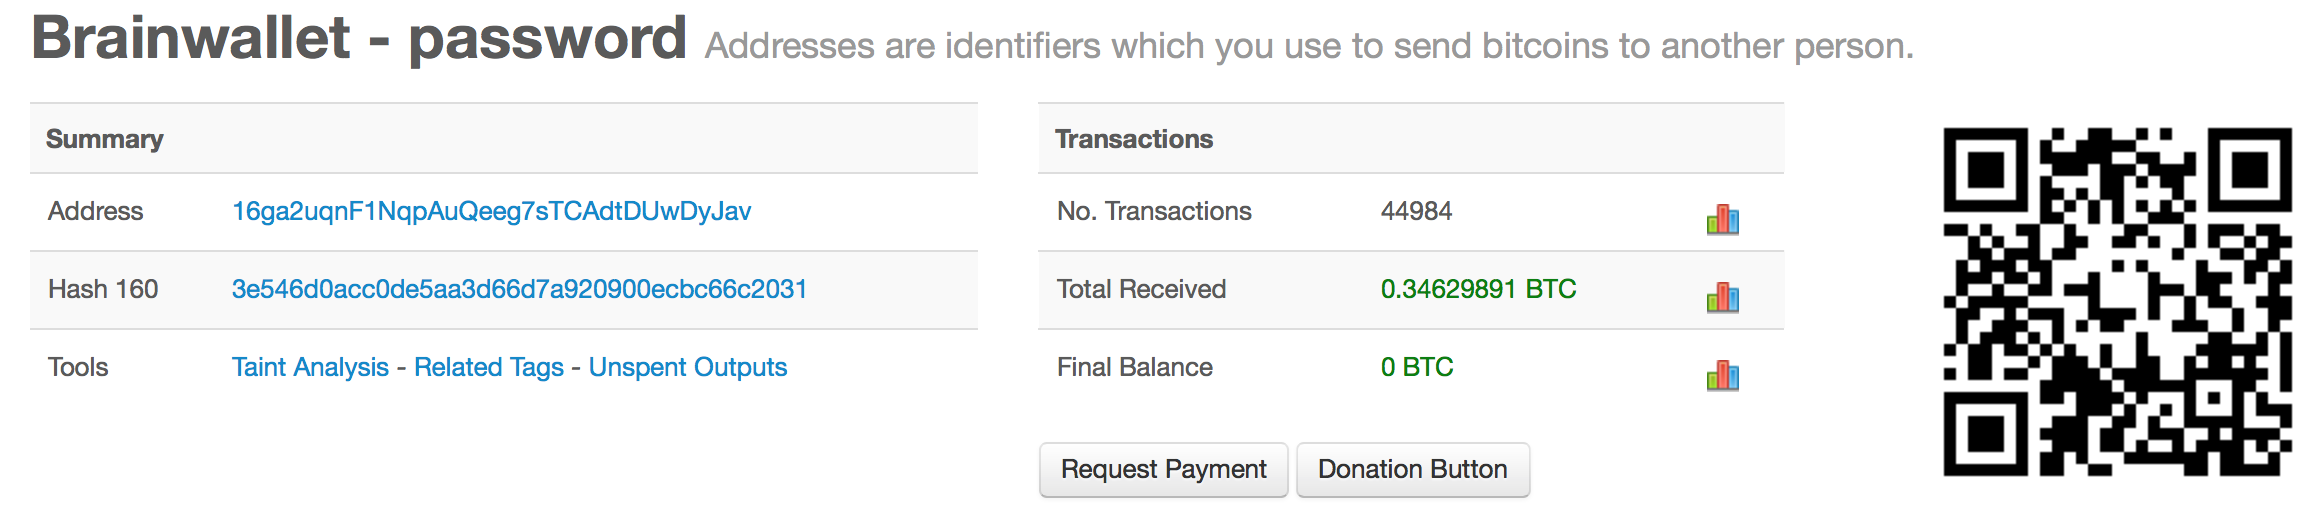
\includegraphics[width=140mm]{./pics/brainwallet-password.png}
	\caption{Brainwallet generated by password ``password''}
	\label{fig:brainwallet_password}
\end{figure}

Brain wallet users are normally urged to use strong passwords or passphrases. Websites provide a brain wallets generation service often using Figure \ref{fig:password_strength} to tell the users what is a strong password. However, this figure is a little bit misleading which makes users feel it is safe to use brain wallets with a passphrase. We have actually cracked quite a few such passphrases. In this thesis we mainly focus on speed optimization of password guessing.

\begin{figure}[h!]
	\centering
	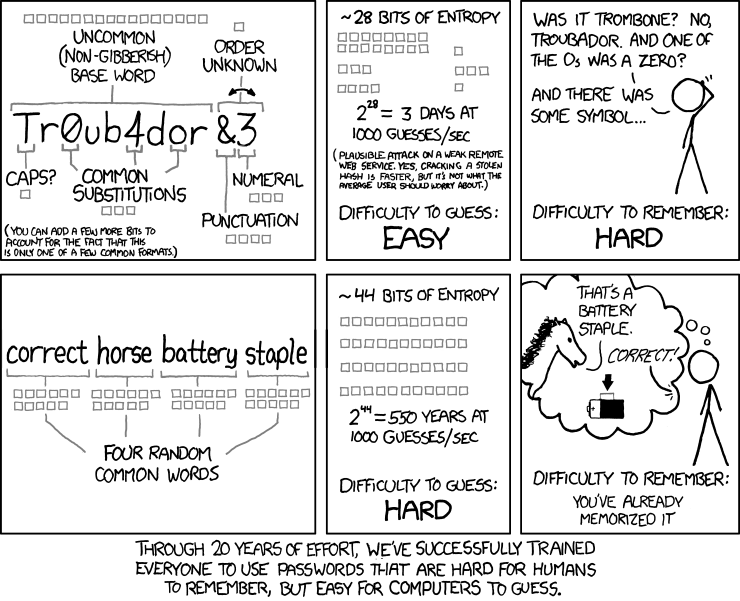
\includegraphics[width=140mm]{./pics/password_strength.png}
	\caption[Password strength comparison between using password and passphrase]{Password strength comparison between using password and passphrase, source: \url{xkcd.com}. This cartoon gives us good advice about how hard it is to guess one user's passwords. But sometimes the speed of guessing can be misleading.}
	\label{fig:password_strength}
\end{figure}

In the next section we will discuss about existing methods of Bitcoin elliptic curve implementation, benchmarking the state-of-art attack and show an improved method of running the attack with much faster speed on a laptop. 
\subsection{Related Work} \label{sec:brainwalletRelatedWork}
We are not the first ones try to crack Bitcoin brain wallets; a lot of other security researchers are doing it. Many victims have found their money stolen and posted it in forums. The first ethical/research brain wallet cracker was announced publicly in a recent hacking conference DEF CON 23 (Aug 2015). Ryan Castellucci, a whitehat hacker, presented his research on cracking brain wallets, and also published his software \cite{RyanDefcon}. Ryan's attack was done on an Intel i7 PC with 4 hyper-threaded cores. The attack speed can reach approximately 16,250 passwords per second on each thread and he had cracked more than 18,000 brain wallet addresses.

The software Ryan has published uses an existing open source secp256k1 Bitcoin elliptic curve implementation mainly written by Pieter Wuille, one of Bitcoin core developers. This implementation is widely used in Bitcoin clients and is considered the current best in terms of code level optimization (detailed benchmarks are given in  table \ref{table:benchmark_msi_affine}).

Later Vasek et al. published their cybercrime analysis results on brain wallets addresses cracked using Ryan's software implementation in FC 2016. Their work was more focused on brain wallets usage measurements and did not try to improve the speed of the attack.

\part{The Path to Better Software Algebraic Cryptanalysis} \label{Part2}
\chapter{Contradiction Immunity and Application to GOST}\label{ch:GOST}

%DEScourtois
%courtois2008algebraicKeeLoq


In this chapter, we will introduce a key fundamental notion of Contradiction Immunity of a block cipher and a related notion of SAT Immunity. These notions lead to new computational optimization problems in cryptography. The main idea is to look for an optimal software guess-then-determine attack. We also provide a concrete example of how this attack can be accomplished on the Russian federation encryption standard GOST with a SAT solver. 

\section{Contradiction Immunity and SAT Immunity}

\subsection{Software Algebraic Attack with SAT Solver} \label{sec:SoftAlgAttackSAT}
As we discussed in Section \ref{sec:CrytanalysisGOST}, due to the self similarity property inside the cipher structure, the problem of solving full GOST can be reduced to solving an 8 rounds GOST \cite{gostac}. In Section \ref{sec:ACReduction} we described algebraic complexity reduction and the notion of amplification in general. In this section we look at how the amplification principle can be applied to GOST. Here the question is what is the best possible software attack with tools such as the ElimLin algorithm \cite{AlgSnowCourtoisDebraize,DEScourtois,ElimLinR}, SAT solvers \cite{OptimiPaper,BardCourtoiJeffersonConv}, Gr\"{o}bner bases \cite{grobner} and others \cite{SemaevSparseJournalPaper}. In all these algorithms we observe the phenomenon of amplification in various forms. For example, we can study and count linearly independent linear equations and try to amplify their number
by the ElimLin algorithm \cite{AlgSnowCourtoisDebraize,DEScourtois,ElimLinR}.
%this is still almost black box: non-linear operations are seen as black boxes... or grey boxes...
%However as previously explained, amplification can become very high.
When the ElimLin algorithm is itself the last step of the attack, or if the SAT solver is the last step of the attack, this amplification phenomenon becomes very important. We observe an avalanche-like phenomenon where more and more new linear equations are generated in the ElimLin algorithm, until the system is solved. Similarly, with a SAT solver there is a point of phase transition
where the problem becomes really easy to solve. If we want to understand algebraic cryptanalysis, we need precisely to work
on this phase transition phenomenon itself. What happens after this threshold, when the problem is just very easy to solve,
is less important.

In this chapter we focus more specifically on cryptographic attacks with SAT solvers, and on GOST, which is a nice example
of a weak government standard cipher with excessively poor diffusion. There are two main approaches in SAT cryptanalysis
or two main ways to break a cipher with a SAT solver:

\begin{enumerate}
	\item
	{\bf The SAT Method:}
	Guess $X$ bits and run a SAT solver which,
	if the assumption on $X$ bits is correct, takes time $T$.
	Abort all the other computations at time $T$.
	The total time complexity is about $2^{X}\cdot T$.
	\item
	{\bf The UNSAT Method:}
	Guess $X$ bits and run a SAT solver which,
	if the assumption on $X$ bits is incorrect,
	finds a contradiction in time $T$
	with large probability $1-P$ say 99$\%$.
	
	With a small probability of $P>0$,
	we can guess more key bits
	and either find additional contradictions
	or find the solution.
	
	The idea is that if $P$ is small enough, the complexity of
	these additional steps can be less then the $2^{X}\cdot T$ spent
	in the initial UNSAT step.
	
	\item
	{\bf A Mixed UNSAT/SAT Attack:}
	In practice maybe $P$ is not as small as we wish, and therefore we may have
	a mix of SAT and UNSAT methods:
	where the final complexity will be a sum of two (or more) terms, none of which can be neglected.
	We will see a very nice example of
	how a combined attack can be better
	than any of SAT and UNSAT methods in isolation
	in Section \ref{section:Fact8R4KP_94_SATMethod}.
\end{enumerate}

Note that the UNSAT method does not belong to amplification, but it reduces solving complexity by quickly rejecting wrong guesses. This can be seen as cutting the branches in a binary search tree, and finally makes finding contradictions easier by a SAT solver. The idea behind the UNSAT method also appears in Cryptanalysis history. For example, Turing's Bombe machine which explored the daily setting of the Germany Enigma, used a similar idea by rejecting wrong guesses which lead to a contradiction (to be precise, one letter is encrypted to itself).

\subsection{Contradiction Immunity and SAT Immunity}
In order to quantify the resistance of a cipher against the two attacks described above,
it is natural to define the two following numbers:

\begin{mydef}
	[Contradiction Immunity or UNSAT Immunity]
	We define the
	Contradiction Immunity of
	a given cipher
	and for $M=1$ plaintext/ciphertext pairs
	of the
	cipher as being
	the smallest possible
	number of key bits
	which can be fixed so that
	given $M=1$ P/C pair we
	can obtain a contradiction
	with probability at least
	50$\%$ by just
	examining the logical consequences
	of these key bits.
	We require this contradiction
	to be found in a very short time,
	less than 1 second for
	the best SAT solver available.
\end{mydef}

\begin{mydef} \label{DEF:SAT_IMMUNITY}
	[SAT Immunity or Satisfaction Immunity]
	We define the
	SAT Immunity of
	a given cipher
	and for $M$ plaintext/ciphertext pairs
	of the
	cipher as
	being the smallest possible
	number of key bits
	which can be fixed so that
	given $M$ P/C pairs we
	can compute the secret key by
	the best available SAT solver in a relatively short time,
	say less than 1000 seconds.
\end{mydef}

These notions are as precise as they can be. Although they depend on the software used, but it is not to excessive extent. Because we can only hope to provide upper bounds for this quantity by concrete attacks with concrete software, it makes sense to use the best available software and improve these bounds slightly each time as the software improves.
Importantly, we should consider that the first notion is much more robust and more fundamental: it expected to depend only on the connections between the components with the ``optimal'' subset of key bits, we do not expect that the contradiction will be found by examining too many other bits, but just by simple step-by-step local analysis.
We also expect that the time taken to find a contradiction will be essentially zero and will not depend too much on the software used. Some SAT solvers are good at solving contradiction problems (known as UNSAT problems), but in this case, we believe it is not very important which SAT solver will be used to obtain the contradiction.
In contrast, the SAT Immunity can only be determined by somewhat ``solving'' the whole cipher,
with the avalanche effect.
Unless we are able to determine all the bits in the whole cipher,
we do NOT know if the cipher is really solvable.
Our experience shows that the results for the second notion will depend
a lot on the SAT solver software used and where some software works well,
some other does not seem to work at all \footnote{Performance of a SAT solver solving cryptanalysis problems is largerly depends on how the cipher is represented using CNF format. The number of variables and constrains in a SAT problem can dertimin the solving complexity and each solver perfroms differently on different problem.}. This is because when solving UNSAT problems (espically in crypanalysis) a contridiction can be easily found in early round of the encryption, thus the solving complexity is very low and problem normally get solved within seconds. Even different algorthims perform differently on a given problem, in most of the case, the difference is very small in order to find a contridiction. However when solving a SAT problem the aim is to solve the whole equeation system with and find the key, (in Definition \ref{DEF:SAT_IMMUNITY}, we set solver time out as 1000 seconds). Due to the complexity of the problem, some SAT solvers can't find any solution within the time limit.

A small technicality is that in order to determine the key uniquely
in many ciphers where the key size is bigger than the block size,
it is necessary to use some $M>1$. Because in order to find a unique solution within a multivariable equations system, the number of equations should be larger than the number of unknowns, otherwise there could exist multiple solutions in the equation system. However, for the first notion, for finding contradictions,
we can frequently limit ourselves to considering the case where $M=1$ because most of the case contridiction can be found easily within early round of the encryption if key bits are wrong.


\subsection{Applications of UNSAT/SAT Immunities}
\noindent 
{\bf Cryptanalysis}. %Intended Application.}
SAT and UNSAT immunities will allow us to evaluate the security of the cipher against cryptanalytic attacks with a SAT solver. Upper bounds we obtain do translate, more or less, as we will see,
into concrete attacks with a complexity of about $2^{X}$. The two figures will also indicate which of the three
strategies (SAT/UNSAT/Mixed) is more likely to work.

\noindent
{\bf Design of Block Ciphers}.
It is easy to see that the designer of a cipher can very effectively lower-bound these quantities.
This will be achieved by making sure
that each S-box in each round
influences as many S-boxes as possible in the next round.
This is not all very different to designing a cipher
which is provably resistant to linear and differential cryptanalysis.
In 2007, Schneier once claimed that ``Against differential and linear cryptanalysis, GOST is probably stronger than DES''
\cite{schneier2007applied}.
Therefore we should also expect that Contradiction Immunity
of DES and GOST are comparable.
Happily, similar attacks with SAT solvers have been developed
for both DES \cite{DEScourtois} and GOST \cite{OptimiPaper}.
In fact, it is obvious that the diffusion in DES
is much better than in GOST and so is the Contradiction Immunity in DES.
However, we need to be careful about drawing any conclusions
and direct comparisons do not mean much.
If the contradiction immunity is 78 for 8 out of 32 rounds of GOST with 3 P/C pairs and 256-bit keys,
is it better or less good
than contradiction immunity
being 20 for 6 rounds out of 16 of DES with 1 P/C pair and 56-bit keys?
It is very hard to say.

\section{Applying SAT/UNSAT Immunity to GOST and DES}

\subsection{Application to DES}
 In DES the key bits are spread more or less uniformly in different rounds, and they tend to repeat many times. Therefore it is difficult to choose really good sets of bits using our discovery method and, for now, we just report upper bounds obtained when choosing
the key bits at random, and letting the SAT solver do the job. 

There are multiple ways of write DES S-boxes into algebric equations which will leads to different solving complexity for AC solving stages. In 2007 Courtois and Bard studied the best s-box encodings with low I/O degrees \cite{courtois2007algebraicDES}, and provided ready software for generating such equations and solve the SAT problem using MiniSat \cite{minisat}. Our experiments set up uses the same software for generating DES equations, and the results are obtained by using a better performing SAT solver CryptoMiniSat 2.92 \cite{CryptoMiniSat}.

For Contradiction Immunity our experiments use 8 rounds of DES with 1 P/C pair. Using random generated key and fix a large number of the key bits $x$, then reduce $x$ until we no longer able to obtain a contradiction with probability at 50\% using SAT solver within 1 seconds. Finally, report the smallest possible number of key bits. For SAT immunity, the experiment was using 8 rounds of DES and 1 P/C pair, random key and random fixed key bits. We run CryptoMiniSat until we obtian the smallest possible number of key bits that can be fixed so that we can solve the converted SAT problem and obtain the secret key within 1000 seconds.

Our final results are:
\begin{enumerate}
	\item The Contradiction Immunity
	%is at most 28 for 6 rounds of DES and it
	is at most 44 for 8 rounds of DES.
	\item
	The SAT Immunity
	%is at most 17 for 6 rounds of DES and 1 KP and it
	is at most 34 for 8 rounds of DES and 1 P/C pair.
\end{enumerate}

DES has key size of 56 bits, for SAT method, we have to fix 34 bits (request $2^{34}$ GOST encryption) and solve within 1000 seconds by a SAT solver. Our PC can run approximately $2^{22}$ 8 rounds DES encryptions per seconds. The total time complexity of solving 8 rounds of DES using 1 P/C pair is larger than brute force. For ultra low-data complexity attacks, 8 rounds of DES seem already secure or secure enough.

\subsection{Contradiction Immunity of GOST} 
Now we are going to provide some results on the Contradiction Immunity and SAT Immunity of GOST. These results are constructive upper bounds.

First we started in a similar set up as DES, with random selected key bits for guessing. The initail Contradiction Immunity we got was about 128. Previous cryptanalysis work on GOST done by Coutrios in 2012 \cite{gostdc2} analysed the internal structure on GOST and how key bits and S-boxes are connected for each round of the encryption. Courtios' work \cite{gostdc2} shows that GOST splits very neatly into two nearly independent ciphers with 128-bit key each, which are only loosely connected. With this idea it is easy to understand why Courtois' original attack on 8 rounds of GOST with complexity of $2^{120}$ \cite{gostreport} seems plausible and natural. Randonly guessed key bits will not create a closely connected structure, thus the chance to find a contridiction for wrong guesses become harder compared to closely connected key bits.
%% full version maybe %%, and that we do not expect much faster such attacks to exist.
However, our research found that it is much lower than 128,
and much closer to 64. 
\begin{lemma}
	The Contradiction Immunity for 8 rounds of GOST is at most 78.
\end{lemma}


{\bf Notation, cf. Figure \ref{Gost81optimal4KPUNSAT78}}:
We denote by $S^{1}3$ just 1 higher ranking bit at S-box 1 in a given round.
Similarly we denote by $S_{3}3$ the 3 lower ranking bits of S3.

\begin{figure}[h]
	\centering
	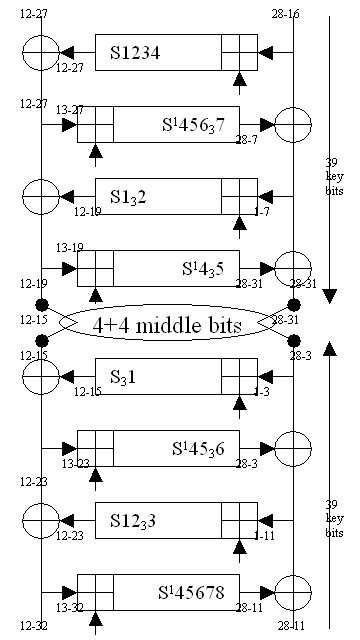
\includegraphics[width=60mm]{./pics/gost81optimal4KP.jpg}
	\caption[Our best set of 78 bits for UNSAT]{Our best set of 78 bits for UNSAT. We denote by $S^{1}3$ just 1 higher ranking bit at S-box 1 in a given round.
		Similarly $S_{3}3$ the 3 lower ranking bits of S3. $\boxplus$ is the modulo $2^{32}$ operation. Best set we found is fixing key bits 0-15,47-58,64-70,111-114,128-130,175-182,192-202,239-255. The inner rounds output bits that are determined by these key bits are showed in the figure   }
	\label{Gost81optimal4KPUNSAT78}
\end{figure}

We have constructed and tried many different sets aiming at a contradiction in the middle. Such sets can be constructed using simple heuristic method such as hill-climbing method \cite{selman2006hill} with a staring point contructed by humman. 
Our best set is as follows (cf. Figure \ref{Gost81optimal4KPUNSAT78}):
0-15,47-58,64-70,111-114,128-130,175-182,192-202,239-255.
The contradictions can be found in time of 0.06 s
with CryptoMiniSat 2.92 software \cite{CryptoMiniSat}
with a probability of about 50 $\%$.

\subsection{SAT Immunity of GOST}
It turns out that a set which is good for UNSAT is typically NOT good at SAT.
No SAT solver software we dispose of is able to find the missing bits if the 78 bits of Figure \ref{Gost81optimal4KPUNSAT78} are fixed.
Happily we have found sets which are very good at SAT and they are in fact smaller than 78.
Our best result is as follows:

\begin{lemma}
The SAT Immunity for 8 rounds of GOST and 4 P/C pair is at most 68.
\end{lemma}
	
We use the following set of bits
depicted on Fig \ref{Gost81optimal4KPSAT68Bits}
0-15,51-55,64-66,128-130,179-183,192-207,224-231,244-255.
All the remaining 256-68 bits can be determined in time of
about 400 seconds
using GOST encodings described in Section \ref{sec:GOSTStructure}
and with CryptoMiniSat 2.92.

From here a naive ``SAT strategy'' attack on GOST would be to run
a SAT solver for 400 seconds $2^{68}$ times.
This would be about $2^{99}$ GOST encryptions.


\begin{figure}[h!]
	\centering
	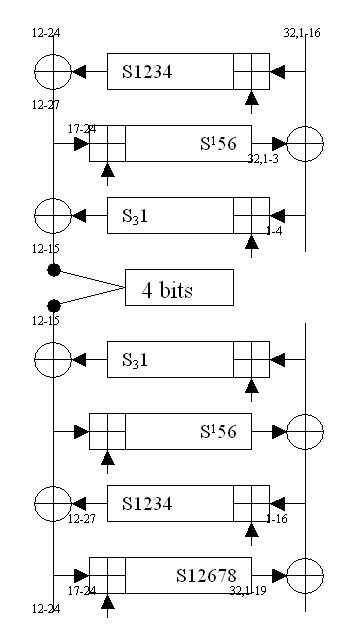
\includegraphics[width=60mm]{./pics/gost81optimalSAT4KP.jpg}
	\caption{Our best set of 68 bits for SAT}
	\label{Gost81optimal4KPSAT68Bits}
\end{figure}

%\newpage

%\subsection{Application to Full 32-round GOST}
\subsection{Low Data Complexity Meet-In-The-Middle Attack for 8 Rounds GOST}
\label{section:Fact8R4KP_94_SATMethod}
In our attack with 4 P/C pairs we want to find a contradiction for all the 4 pairs simultaneously.
This will be easier than contradiction with 1 P/C pairs we studied previously.
This leads to the following improved attack which mixes the SAT and UNSAT strategies.

\begin{enumerate}
	\item
	We use our set of 68 bits as
	on Figure \ref{Gost81optimal4KPSAT68Bits}. %and in Fact \ref{SATImm8Rounds}.
	\item
	We run the software $2^{68}$ times for all possible assignments of the 68 bits.
	\item
	Computer simulations
	with the timeout of 7 seconds,
	a proportion of $1-2^{-5}$ of cases on 68 bits terminates with UNSAT
	within 2 s on average.
	\item
	Overall, we only need to run a proportion of $2^{-5}$ of all the $2^{68}$ cases
	for as many as 400 seconds;
	in other cases it simply terminates automatically within 2 s
	which is $2^{23}$ GOST encryptions on the same CPU.
	\item
	Assuming that all the other cases run for 400 s (some still terminate earlier)
	our conservative estimate of the attack time is
	$2^{68+23}+2^{68+31-5}\approx 2^{94}$ GOST computations.
\end{enumerate}

\section{Conclution}
In this chapter, we discussed algebraic cryptanalysis using SAT solver as solving stage and it's application to break 8 round GOST. We introduced a new notion of Contradiction Immunity and a related notion of SAT Immunity. These definitions lead to new computational optimization problems in cryptography, which can be seen as looking for an optimal software guess-then-solve attack. We provided our best optimizations found which were constructed following a sort of meet-in-the middle strategy. Our key result is that the Contradiction Immunity for the GOST cipher is quite low, about 78, for 8 rounds. 

The main contribution of this chpater is not just providing a bound on the two Immunity figures, but to provide concrete sets of bits based on which we can build concrete attacks on the given cipher. Theses sets are fundamental in being able to improve the time complexity of 8 rounds of GOST attack from $2^{120}$ to $2^{94}$. 


\chapter{Algebraic Cryptanalysis of Simon}\label{ch:SIMON}
In Chapter \ref{ch:GOST} we have introduced the notion of contradiction immunity and SAT immunity. We have shown how an optimized guess-then-solve attack can be done on GOST. In this chapter, we are going to explore how to improve algebraic attack with well chosen data. Our target is the new NSA block cipher Simon\cite{NSAciphers}. The lightweight block cipher Simon was introduced by NSA in 2013 and later submitted to ISO to become an international standard. Similar to GOST, Simon has very low diffusion and small S-boxes, which makes it an excellent target for algebraic cryptanalysis. Our aim is to use the very rich algebraic structure
with additional data provided ( e.g. pairs $\{(P,P'),(C,C')\}$ which
follow a certain highly probable truncated differential property) in order to solve
the underlying multivariate system of equations. We attempt to solve the system
by either using a SAT solver (after converting the system to its corresponding
CNF-SAT form with the Courtois-Bard-Jefferson method \cite{BardCourtoiJeffersonConv}) or by the ElimLin algorithm \cite{FourMNL,OptimiPaper,OptimiPaper2}.
We are able to break up to 10 (/44) rounds of the cipher using
a SAT solver and the usual guess-then-determine techniques.
Surprisingly, in most cases we are
able to obtain the key without guessing any key bits
when truncated differentials are used.
This is a very remarkable result as it gives a good hope that the attack will scale up well for a larger number of rounds. This is possibly due to the very low non-linearity of the cipher and suggests that it is worth studying a specific strategy for P/C pairs which have a certain structure and decrease even more the non-linearity of the system by introducing
more linear equations (e.g. truncated differential properties)
until the key can be obtained even for a larger number of rounds. We will discuss in details our results in Section \ref{Sec:SimonResult}.


\section{How to Write Simon Equations}
In Figure \ref{fig:ch3ACmodeling} we showed a general example of modelling a block cipher into MQ equation systems. Here we give a concrete example for writing Simon64/128 in a single round.

Recall the Simon structure in Figure \ref{fig:SIMONroundfn}, let $ek_i$ be the $i$-th key bit used in $Nr$-th round of Simon64/128 encryption. The 32-bit key has a binary representation: $ek=\left( ek_{31},ek_{30}...ek_{0}\right) $. Let $ZR^{Nr}_i$ and $ZL^{Nr}_i$ be the $i$-th bit of $Nr$-th round right and left side input, and similarly $ZR^{Nr+1}_i$, $ZL^{Nr+1}_i$ for the $i$-th bit of output. Then we have:

\begin{center}
$ek_0+ZL^{Nr}_{30} + ZR^{Nr}_0+ZL^{Nr+1}_0+ZL^{Nr}_{24}*ZL^{Nr}_{31} = 0$\\
$ZR^{Nr+1}_0+ZL^{Nr}_0 = 0$ \\
$ek_1+ZL^{Nr}_{31} + ZR^{Nr}_1+ZL^{Nr+1}_1+ZL^{Nr}_{25}*ZL^{Nr}_{0} = 0$\\
$ZR^{Nr+1}_1+ZL^{Nr}_1 = 0$ \\
$\dots$ \\
$ek_{31}+ZL^{Nr}_{29} + ZR^{Nr}_{31}+ZL^{Nr+1}_{31}+ZL^{Nr}_{23}*ZL^{Nr}_{30} = 0$\\
$ZR^{Nr+1}_{31}+ZL^{Nr}_{31} = 0$ 
\end{center}

Similarly, one can simply write equations for the key extension function, cf. \cite{NSAciphers}. More details can be found in our Simon implementation code (including equation generator for all versions) which is available online \cite{SongSimonSpeckGithub}.
\section{Differential-Algebraic Cryptanalysis of Simon}\label{Sec:DAcSimon}

We evaluated the security of Simon against algebraic attacks under the following
three settings (cf. Fig. \ref{ThreeScenarios}), where S=Similar and R=Random
as explained in the introduction.

\begin{itemize}
	\item \textbf{Setting 1:}  Known Plaintext Attack. Random P/C pairs are available (RP/RC). 
	\item \textbf{Setting 2:} One type of Chosen Plaintext Attack.  Random P/C pairs are available with plaintexts of low Hamming distance (SP/RC).
	\item \textbf{Setting 3:} Some form of Chosen Plaintext and Ciphertext Attack. Random P/C pairs which satisfy a truncated differential property in the input and output of the reduced-version of the cipher we study.  (SP/SC) %More random P/C pairs are generated and used. 
	% \item \textbf{Setting 3':}(SP/SC)' Random P/C pairs which satisfy a truncated differential property in the input and output of the reduced-version of the cipher we study. Then we generate more such pairs by using pairs with similar plaintexts (low Hamming Distance)
	%    such that ciphertext pairs lie in the truncated differential mask.
\end{itemize}

\begin{figure}[!h]
	\vspace{-0.2cm}
	\centering
	%{\epsfig{file = three_scenarios.eps, width = 7.5cm}}
	\includegraphics*[width=60mm]{./pics/three_scenarios2.jpg}
	\caption{Our three attack scenarios}
	\label{ThreeScenarios}
	\vspace{-0.1cm}
\end{figure}



%\begin{figure}[h!]
%    \centering
%    \includegraphics{three_scenarios.eps}
%    \caption[width=0.2]{Our three attack scenarios}
%    \label{setting}
%\end{figure}

Setting 1 is the simplest setting for understanding how many rounds of Simon
can be broken by simple techniques, assuming availability of
a few P/C pairs. This setting helps us to understand the maximum number of rounds we
can break by guessing as few key bits as possible and using as few  P/C
pairs as possible. It is a non-trivial step in order to set the benchmark for attacking larger number of rounds.


Setting 2 is a form of known-plaintext attack. Setting 2 requires the existence of P/C pairs with plaintexts
of low Hamming distance (or similar plaintexts)
such that many variables are eliminated in the first few rounds due to weak
diffusion. By eliminating some variables from the initial equations we expect that
the system will be solved faster using any solving technique. This is a form of
chosen plaintext attack.

Lastly, Setting 3 assumes the existence of P/C pairs

\begin{center}
	$\{(P_1,C_1),(P_2,C_2),...,(P_n,C_n)\}$
\end{center}

such that
$P_i\oplus P_j \in \Delta P$ and $C_i\oplus C_j \in \Delta C$, for
all $1\leq i,j \leq n$ and some truncated differential masks $\Delta P,\Delta C$
of low Hamming weight which holds with comparatively high probability.
In our attacks we always use 2 pairs which satisfy a given truncated
differential property and then more P/C pairs are generated by using the
first 2 plaintexts and computing the encryptions of new plaintexts which have small Hamming distance from the
first ones. 

The difference
from Setting 2 is that in this case we also eliminate variables
from the last rounds of the cipher, expecting that the system is even easier to solve. In this
attack, we assume (to make it simple) that the entire codebook is available and thus the
data complexity is $2^{64}$.

In all of our attacks we start with an 8-round truncated differential property (see Section \ref{sec:differentialCry} and more details can be found in \cite{TheoPhD}) $\Delta=[00000222 00000080]$
with 4 active bits found by heuristic method:

\begin{equation}
Prob(\Delta\rightarrow \Delta)\simeq2^{-20.51}
\end{equation}

The mask $[00000222 00000080]$ denotes the set of $2^4-1$ possible differences,
excluding the zero difference.
Our detailed results and discussion will be presented in the following section.

\section{Algebraic Attacks experiments and results} \label{Sec:SimonResult}
We run experiments using SAT solvers and ElimLin Algorithm on a machine with the
following characteristics
\begin{small}
\begin{itemize}
	\item CPU: Intel i7-3520m 2.9GHz
	\item RAM: 4G
	\item OS: 64-bit Windows 8
\end{itemize}
\end{small}
Our open source implementation of Simon also includes an equation generator which generates an algebraic equitation system for n round Simon encryption. Once the equation is generated, we use Nicolas Courtois' software \cite{EquationSolving} to either solve the system by ElimLin or convert to CNF file and then solve by a SAT solver. For the reader to check and verify our results, here are the command lines we used to get our experimental results, software are available online \cite{simonref,EquationSolving} :
\begin{small}
\begin{itemize}
	\item Equation generation: Simon.exe NumberOfRounds fixedKey  
	\item ElimLin: xl0.exe /deg2 fileName 
	\item SAT solver: xl0.exe /deg2 /sat /bard /timeout600 /cryptominisat64296 fileName
\end{itemize}
\end{small}
\subsection{Experiments with 2 P/C pairs}
The initial benchmark experiments were done with only 2 P/C pairs and solved by a SAT solver using 8 round Truncated differential mask $[00000222 00000080]$ $\Rightarrow$ $[00000222 00000080]$. Table \ref{tab:example1} presents our 2 P/C pairs experiment results. The average time (in seconds) taken $T_{average}$
to solve the underlying problem
by a SAT solver is presented, while the time complexity $C_T$
(in terms of Simon encryptions) is
computed by the following formulae,

\begin{equation} \label{EQ:time_comp}
C_T=2^{k}\times2^{log_2(T_{average}*N_{8REnc})},
\end{equation}

where $k$ is the number of bits we guess initially, $N_{nREnc}$ is the number of n round Simon encryptions the experiment PC can run in 1 second.

\begin{table}[!hh]
	\caption[Best results obtained by a SAT solver using 2P/C pairs]{Best results obtained by a SAT solver using 2P/C pairs for 8 rounds of SIMON64/128. $k$ is the total number of randomly guessed key bits. The time complexity for guessing is $2^{k}$. $\#$(P/C) shows the number of plaintext-ciphertext pairs. $T_{average}$ is the average solving time using a solver. $C_T$  is the total time complexity for breaking the cipher, calculated based on equation \ref{EQ:time_comp}. For settings see detail in figure \ref{ThreeScenarios}}\label{tab:example1} \centering
	\begin{tabular}{|c|c|c|c|c|c|}
		\hline
		$\#$(Rounds) & $k$ & $\#$(P/C) & $T_{average}$(s) & $C_T$ & Setting \\
		\hline
		8 & 84 & 2 & 63.76   & $2^{110.08}$ & RP/RC \\
		8 & 80 & 2 & 87.38   & $2^{106.53}$ & RP/RC \\
		\hline
		8 & 75 & 2 & 156.60  & $2^{102.37}$ & SP/RC \\
		\hline
		8 & 75 & 2 & 515.60  & $2^{104.09}$ & SP/SC \\
		\hline
	\end{tabular}
\end{table}

We start from setting 1 using random Plaintext and random Ciphertext pair (RP/RC), until we cannot solve the equations using SAT solver. We successfully break 8 rounds Simon with guessing some key bits. The best result for 8 rounds is fixing 80 key bits with a complexity of $2^{106.53}$. Fixing less than 80 key bits will not be solved by SAT solver within 600 seconds. Then we try setting 2 and setting 3 to compare the results. Setting 2 using selected Plaintext and Random Ciphertext (SP/RC) and setting 3 using selected Plaintext and selected ciphertext (RP/RC) are better than RP/RC. However, the results in Table \ref{tab:example1} show that SP/SC is not performing any better than SP/RC. Both SP/RC and SP/SC are not improving RP/RC a lot. 

The experiment results show that for setting 2 and setting 3, using only 2 P/C pairs cannot provide enough information (additional linear equations) to perform a better attack than RP/RC. In the next subsection we try to increase the number of P/C pairs and compare the results using different settings.

\subsection{Experiments with more P/C pairs}
We start by using more P/C pairs for 8 rounds Simon and we show our results in Table \ref{tab:8RmorePC}. Here we start to record some features of the converted CNF files. In Table \ref{tab:8RmorePC} and other SAT solver results table, $n,s,h$ stand for number of variables, average sparsity (the average number of literals in each clause) and hardness respectively and $m$ is the number of clauses in the converted CNF file.
We define hardness as a number $h$ such that $h^n$ is the running time, where $n$ is the number of variables.
It is known that $h\leq 1.47$ for 4-SAT problems (cf. Table 1 in \cite{semaev})
% explain hardness

\begin{table}[!hh]
	\caption[Best results obtained by a SAT solver for 8 rounds with 6 P/C pairs]{Best results obtained by a SAT solver for 8 rounds with 6 P/C pairs. $n,s,h$ stand for number of variables, average sparsity (the average number of literals in each clause) and hardness respectively and $m$ is the number of clauses in the converted CNF file.
		We define hardness as a number $h$ such that $h^n$ is the running time, where $n$ is the number of variables. }\label{tab:8RmorePC} \centering
	\begin{tabular}{|c|c|c|c|c|c|c|c|c|c|}
		\hline
		$\#$(Rounds) & $k$ & $\#$(P/C) & $T_{average}$(s) & $C_T$ & Setting & $n$ & $x=\frac{m}{n}$ & $s$ & $h$ \\
		\hline
		8 & 45 & 6 & 207.31   & $2^{27.78}$ & RP/RC & 8576	& 6.5118	& 4.2761	& 1.0032 \\
		\hline
		8 & 0  & 6 & 12.21   & $2^{23.76}$ & SP/RC  & 8576	& 6.5065	& 4.2787	& 1.0029  \\
		\hline
		8 & 0  & 6 & 11.84   & $2^{23.57}$ & SP/SC  & 8576	& 6.5513	& 4.2631	& 1.0028 \\
		\hline
	\end{tabular}
\end{table}

%From Table \ref{tab:8RmorePC} we can see that when using more P/C pairs, all the three settings get better results than using 2 P/C pairs in Table \ref{tab:example1}. The improvements for setting 2 and setting 3 are much more larger than setting 1. Setting 2 and setting 3 can break 8R Simon without guessing any key bits.

Then we start to extended the current 8 rounds attack to 9 and 10 rounds. We first extend our 8R truncated differential mask to 9 and 10 rounds as the following:
\begin{itemize}
	\item 9R: $[00000022 00000080]$ $\rightarrow$ $[00022e4c 00000222]$
	\item 10R: $[00000022 00000080]$ $\rightarrow$ $[002eff9a 00022e4c]$ 
\end{itemize}

We manage to break 9 rounds without guessing any key bits and break 10 rounds with some key bits guessing. Our best results are shown in Table \ref{tab:10RmorePC}

\begin{table}[!hh]
	\caption[Best results obtained by a SAT solver]{Best results obtained by a SAT solver. Table set up is the same as table \ref{tab:8RmorePC}. The upper part results are using SP/RC P/C pairs, and the time compliexity for breaking 10 rounds SIMON64/128 is $2^{118.5}$ while using SP/SC with truncated differencial properities gives $2^{98.79}$. The results show the power of using well selected data samples in algerbic cryptanlysis. }\label{tab:10RmorePC} \centering
	\begin{tabular}{|c|c|c|c|c|c|c|c|c|c|}
		\hline
		$\#$(Rounds) & $k$ & $\#$(P/C) & $T_{average}$(s) & $C_T$ & Setting & $n$ & $x=\frac{m}{n}$ & $s$ & $h$ \\
		\hline
		9 & 0 & 6 & 222.50   & $2^{27.9}$ & SP/RC & 9536	& 6.70	& 4.31	& 1.0029 \\
		9 & 0 & 7 & 94.7   & $2^{26.6}$ & SP/RC & 11104	& 6.70	& 4.31	& 1.0024 \\
		10 & 90 & 8 & 346.0   & $2^{118.5}$ & SP/RC & 13952	& 6.90	& 4.32	& 1.0020 \\
		\hline
		9 & 0  & 6 & 24.24   & $2^{24.7}$ & SP/SC  & 9536	& 6.69	& 4.31	& 1.0026  \\
		9 & 0  & 7 & 18.56   & $2^{24.3}$ & SP/SC  & 11104	& 6.70	& 4.31	& 1.0022  \\
		10 & 70  & 10 & 417.73   & $2^{98.79}$ & SP/SC  & 17408	& 6.88	& 4.31	& 1.0022  \\
		\hline
	\end{tabular}
\end{table}

Moreover, assuming Setting 3 we can break 10 rounds by
guessing 70 bits of the key initially with a time complexity of $2^{98.79}$ encryptions.
Note that in SP/SC setting we always generate two P/C pairs which satisfy the truncated differential property, and the rest pairs are generated at random.

The other two settings have failed to produce good results for 10 rounds in reasonable time
and this reflects the power of using pairs which follow strong truncated differential properties. We conjecture that for a cipher of low non-linearity, there exists a certain amount of pairs which depends on the linear relations in the cipher which can be used to break any round.
\subsection{ElimLin Results}
Table \ref{tab:SimonElimlin} presents the results using the ElimLin algorithm for solving the
underlying system of equations.


\begin{table}[!h]
\caption{Best results obtained by a ElimLin Algorithm}\label{tab:SimonElimlin} \centering
\begin{tabular}{|c|c|c|c|c|c|}
  \hline
  $\#$(Rounds) & $k$ & $\#$(P/C) & $T_{average}$(s) & $C_T$ & Setting \\
  \hline
  8 & 0 & 6 & 824.4 & $2^{29.8}$ & SP/RC \\
 \hline
 8 & 0 & 6 & 583.2 & $2^{29.3}$ & SP/SC \\
  \hline
\end{tabular}
\end{table}

ElimLin exploits the existence of linear equations in order to solve the system. We have been able to break up to 8 rounds in Setting 3 without guessing any key bits
initially. Setting 1 fails, while Setting 2 is much weaker than Setting 3. The best
attack we have obtained is of time complexity $2^{29.3}$ encryptions against 8 rounds of Simon and requires pairs which satisfy
the truncated differential property presented in the previous section extended for 8 rounds.

Adding pairs which follow a strong truncated differential property is equivalent to adding linear equations in the system and this
is exploited by the ElimLin algorithm. An immediate improvement is to use additional intermediate truncated differences.
This will also eliminate variables in intermediate rounds and introduce more linear
equations in the intermediate rounds. We conjecture that ElimLin is more powerful
in cases where a strong characteristic is found.
\section{Conclusion}

\chapter{Re-Designing Algebraic Attacks Beyond ElimLin} \label{ch:ElimLIn}
\section{ElimLin Overview}
Our initial algebraic cryptanalysis work on Simon was published in 2014. In 2015,   Raddum \cite{RaddumSimon} published another algebraic cryptanalysis on several different versions of Simon and have broken 16 out of 72 rounds on the largest existing version Simon128/256 using Elimlin with 20 P/C pairs of chosen plaintexts. Raddum's work also shows that ElimLin performs better when adding more P/C pairs.  
%\subsection{UNSAT Method}


%secrypt2016 
%TODO
 
However, it's hard to know what happens when we add even more P/C pairs. This is due to the limited computation power we have. A major difficulty with ElimLin is that so far it has been successful only for relatively simple lightweight ciphers.
For more complex ciphers
%%% full version maybe %%%
%%it is not clear if the attack makes big progress.
it seems to do things which are relatively trivial,
%However until now this has not been formalized.
%We do not know what trivial means.
%for example
e.g. equations generated do not penetrate deeply inside the cipher, or very slowly,
cf. %for example
slide 153 in Courtois' lecture notes \cite{SlidesAlgAllteach}.
% we observe that as the number
%of new linear equations grows,
%these equations penetrate more and more deeply inside the cipher for $2,3,5,\ldots$ rounds.

Our work aims to make some definite progress in the direction of distinguishing between trivial and non-trivial behavior for ElimLin. This is about how deeply an ElimLin attack penetrates. Previous experience shows that ElimLin only starts to work at a certain threshold. Before this threshold, again, nothing non-trivial can be observed even though slow penetration occurs. This is not really apparent in any of the current works or is lost in vast quantities of data generated in the computer simulations. 
%In this paper we are going to be the first to define what non-trivial means.

 In this chapter, we study ElimLin behaviours with randomly selected, increasing number of data samples. By collecting data from large simulations and deeply inspecting the different types of equations generated by ElimLin, we study
 
 \begin{enumerate}
 	\item The growth rate of equations generated by ElimLin
 	\item Where the higher growth rate comes from
 	\item If it is possible to predict when ElimLin will break a cipher
 \end{enumerate}
 
We define a new criterion which shows that it is possible to see that there exist two very different and easily distinguishable patterns in ElimLin. Either the attack follows one pattern, and does nothing non-trivial, or it follows another pattern and it is very clearly doing well. Then we look deeply inside the large number of linear equations found by ElimLin and try to classify different type of equations and identify where the higher growth rate come from.

\subsection{Phase transitions}

It is known that many NP-hard problems are subject to ``phase transition''; with certain parameters that problem is hard, and then it will rather abruptly transition from ``hard'' to ``easy to solve''. This is what we observe with ElimLin. % here. 
Let $K$ be the number of Plaintext/Ciphertext (P/C) pairs used in an ElimLin attack. We are going to discover that at a certain threshold the number of new linear and linearly independent equations
generated at various stages of the attack can follow one curve,
and then switch to another curve with a different asymptotic growth rate.



%\begin{conj}
{\bf Conjecture \ref{ElimLinQuadConj}}
\label{ElimLinQuadConj}
Consider a system of multivariate equations derived from a block cipher (see toy example in \ref{sec:AA} Figure \ref{fig:ch3ACmodeling}). %TODO
Consider a simple known plaintext attack with $K$ Plaintext/Ciphertext (P/C) pairs.
Consider a case such that the cipher is eventually broken by ElimLin, cf. \cite{FastAlg,FastAlg2,ToyRijSer,AlgteachElimLinLab,RaddumSimon}.
The number of new and linearly independent linear equations generated
by the ElimLin algorithm goes through several distinct stages St0-St3:

\begin{enumerate}
	\item[St0]
	Initially it grows linearly with $K$,
	and for certain individual stages of the attack is
	simply equal to 0 and does NOT grow,
	cf. our later $s_i$ notation in Section \ref{ElimLinNotation}.
	\item[St1]
	Then it switches to another curve where
	it grows faster than linearly in $K$.
	%cf Sec. \ref{SuperLinearGrowth}
	\item[St2]
	This is until it reaches a \textbf{saturation} stage where the
	cipher is completely broken by ElimLin.
	Here we sometimes have a very rapid phase transition (cf. Section \ref{BigPictureUpAndDown})
	where the number of equations $s_i$ generated at one stage becomes 0 again
	simply because an earlier stage of the attack reaches a certain threshold where combinatorial explosion
	in additional equations generated
	makes it complete the whole attack and does not requite the next stage to be executed.
\end{enumerate}

\noindent
%Again let $K$ be the number of P/C pairs in an ElimLin attack.
One (old) example from 2007 which shows that the number of equations grows faster than linear
as a function of the data complexity $K$ in ElimLin can be found in Courtios and Debraize's work in 2008 \cite{ToyRijSer}. 

In this chapter we would like to see if this conjecture is verified in real life and how exactly we can approximate different stages of the attack by precise closed formulas which allow us to predict the outcomes of the attack as exactly as possible. 

%A more detailed analysis on equations growth with respect to $K$ can be found in \ref{sec:elimlinJava}


%\newpage

%\section{\uppercase{Our Experimental Setup and Notation}}

\section{How to Predict the Success of ElimLin}

\subsection{Experimental Setup and Notation}
\label{ElimLinSetup}
\label{ElimLinNotation}

We recall the two main and only steps of ElimLin:

\begin{enumerate}
	\item[1] Find $s_i$ linear equations in the linear span, $i=0,1,2,3,\ldots$.
	\item[2a] If $s_i>0$ eliminate some $s_i$ variables,
	increment $i$ and try again Step 1.
	\item[2b] Algorithm terminates when $s_i=0$ for some $i$.
\end{enumerate}

In addition and by convention we are going to define a step $i=0$ which is different than
above, but the same as which is implemented in a common implementation of ElimLin \cite{CourtoisSoftware}.
We will assume that $s_0$ will be the number of linear equations which already appear in the equations,
without executing any linear algebra. This is a convention which allows researchers to distinguish
more easily between a ``misleading'' starting number of variables (which is sometimes artificially inflated due to
methods used for equation generation and formal coding)
and the ``real'' or intrinsic number of variables which is there prior to execution or ElimLin.

%\begin{defi}[ElimLin progress indicators]\\
\begin{mydef}\label{ElimLinProgressParams}
	[ElimLin progress indicators]\\
	Let $V_{start}$, or simply $V$ if there is no confusion,
	be the initial number of variables.
	We define by $s_i$ the number of
	linear/affine equations over GF(2)
	generated at each stage of the algorithm
	where by convention $s_0$ is the number of
	linear/affine equations over GF(2) already present.
	We define
	
	\begin{equation}
	V^i_{broken}=\sum_{j=0}^{i} s_j ~~~~~~~~V_{broken}=\sum_{i=0}^{\infty} s_i
	\end{equation}
	
	where by convention $s_i=0$ if algorithm has reached
	$V^i_{broken}=V$ at an earlier stage.
	We define also
	
	\begin{equation} \label{EQ:unborken}
	V^i_{broken}=V-\sum_{j=0}^{i} s_j
	\end{equation}
	
	and accordingly let
	$
	V_{unbroken}=V-\sum_{i=0}^{\infty} s_i.
	$
	Overall we will say that the algorithm terminates if
	$V_{broken}=V$ and $V_{unbroken}=0$ and we deliberately ignore the fact that
	some variables could be subject to a brute-force step,
	cf. FXL method introudced by Courtois and Patarin \cite{XL2}.
	Overall our goal is to achieve for a certain $i$ that
	\begin{equation}
	\frac{V^i_{broken}}{V_{start}}=1
	~~~~~~~~~~~\mbox{or}~~~~~~~~~~~~
	\frac{V^i_{unbroken}}{V_{start}}=0
	\end{equation}
	
\end{mydef}
%\end{defi}

To give an example of how the experiments are done\footnote{The same software setup has also been used at UCL to run a hands-on student lab session on algebraic cryptanalysis of block ciphers \cite{AlgteachElimLinLab}, which is part of GA18 course on cryptanalysis taught at UCL.}: our Simon implementation is available on GitHub  \cite{AlgteachElimLinLab,CourtoisSoftware}; The ElimLin is executed using one of our implementations of
ElimLin \cite{AlgteachElimLinLab,CourtoisSoftware} which has the nice ability to display on screen the number of linear equations generated at each stage/iteration of the algorithm. Finally we have developed a deep inspection tool in JAVA available online \cite{CourtoisSoftware} which looks deeply inside the equations generated by ElimLin, group the equations based on different selection criteria then provide statistics and predictions for the growth rate of each group. For detailed instructions about how to get these values and full experiment results, see appendix \ref{appendixlabel1}

\section{The Big Picture}
\label{BigPictureUpAndDown}

As already explained in
Conjecture \ref{ElimLinQuadConj}, we expect that there are at least 3 distinct stages in the ElimLin algorithm.
We start with the big picture, by looking at how the value of $V_{unbroken}$ evolves with growing $K$. Here we use a known plaintext setting with no guessed key bits to break 8 round Simon64/128. As we know, adding new P/C pairs to the ElimLin should create a linear growth in the total number of variables. In our experiment setup and SIMON encodings, each P/C pair adds 192 variables to the starting equation system. We study the unsolved variables left at the end of ElimLin run. The results are shown in Figure \ref{ElimLinUnrokenCurveUpDownSimon8} with a fitting curve using polynomial regression.

\begin{figure}[h!]
	\vspace{-0.2cm}
	\centering
	\includegraphics*[width=150mm,height=14cm]{./pics/Figure6-1.png}
	\caption[Number of variables when ElimLin terminates  $V_{unbroken}$
		for 8 rounds of Simon 64/128 obtained with our experiments.]{Number of variables when ElimLin terminates  $V_{unbroken}$
			for 8 rounds of Simon 64/128 obtained with our experiments.
		When $K \leq 16$ the unbroken variables increase. Variables solved by ElimLin are less or equal than variables increased due to added new P/C pairs. We consider this is St0 in
		Conjecture \ref{ElimLinQuadConj}. When $ 16 < K \leq 50 $ the unsolved variables start to slowly decrease, we consider this is St1. When $ K > 50 $ unbroken variables decrease much faster than linear and we consider this stage as St2.}
	\label{ElimLinUnrokenCurveUpDownSimon8}
	\vspace{-0.1cm}
\end{figure}

In Figure \ref{ElimLinUnrokenCurveUpDownSimon8}, we can see a distinction between St0 and St1. In St0 the number of unbroken variables grows linearly with $K$. When the curve switches to St2, the number of unbroken variables grows much more slowly. This curve shows that the number of new generated equations is growing much faster than linear in St1 and causing a lot of variables eliminated by ElimLin. Clearly, St1-2 is the most fundamental stages of ElimLin. It contains the phase transition from ``hard" to ``easy".



\subsection{On Growth Rate in ElimLin}
\label{SuperLinearGrowth}
In section \ref{BigPictureUpAndDown} we looked at the overall unbroken variables as a function on $K$ P/C pairs. We know the total varible growth linearly with $K$. So based on equation \ref{EQ:unborken} we know the solved variables increase faster than linear in St2. Here we look at the growth rate on the number of newly generated equations as a function of $K$.  On Figure \ref{fig:ElimLinQuadConjExampleSimon8r123} we show that early stages $s_{0,1,2,3}$ (see definitions in Section \ref{ElimLinNotation}) of ElimLin algorithm on 8 rounds of Simon block cipher grows linearly. This means at the early stage, ElimLin algorithm only finds trivial equations and the results are very easy to predict. 

Moreover a linear progress curve would not be sufficient to break the cipher, 
because the number of variables also increases linearly. 
In addition, initially the attack starts with a handicap: below a certain threshold no equation exist at all, or many types of equations (equations with similar size and
characteristics, topic which we will study later) seen in larger simulations do not yet exist at all (0 equation found).



\begin{figure}[!h] 
	\vspace{-0.2cm}
	\centering
	\includegraphics*[width=160mm, height=14cm]{./pics/s1s2s3asK.png}
	\caption[Number of linearly independent equations generated at step 1,2,3
	of the ElimLin algorithm]{Number of linearly independent equations generated at step 1,2,3
		of the ElimLin algorithm
		for 8 rounds of Simon 64/128. The results show in step 1,2,3 of ElimLin, number of equations increase linearly and does not create the faster than linear growth we oberseved in Figure \ref{ElimLinUnrokenCurveUpDownSimon8}.}
	\label{fig:ElimLinQuadConjExampleSimon8r123}
	\vspace{-0.1cm}
\end{figure}

In Figure \ref{fig:ElimLinQuadConjExampleSimon8r4}, we show the number of linear equations generated at step 4 of the ElimLin algorithm for 8 rounds of Simon block cipher. We have then produced a polynomial interpolation for this data series. It grows faster than linear which is the first stage of the attack with a positive and non-trivial outcome. 

\begin{figure}[!h]
	\vspace{-0.2cm}
	\centering
	\includegraphics*[width=150mm,height=12cm]{./pics/s4asK.png}
		\caption[Number of linearly independent equations generated at step 4]{Number of linearly independent equations generated at step 4
			of the ElimLin algorithm
			for 8 rounds of Simon 64/128. Step 4 equations appear at K=16, and shows faster than linear increase when $K > 50$, this algains with the stages appeared in Figure  \ref{ElimLinUnrokenCurveUpDownSimon8} when curve switch from St0-1 and St1-2. }
	\label{fig:ElimLinQuadConjExampleSimon8r4}
	\vspace{-0.1cm}
\end{figure}

Note that we start to have $s_4 > 0$ when $K >16$. This also aligns with Figure \ref{ElimLinUnrokenCurveUpDownSimon8} when we see a switch from St0 to St1. 
This is where ElimLin starts to create a growing number of equations which we want to 
grow faster than linear. 
 
\subsection{Deep Inspection}
We start to wonder \textbf{which} set or type of equations in $s_4$ grows faster than linear. 
Up till now we still don't know what kind of equations are found when ElimLin starts to work, and we conjecture that precisely those equations with a fast growth rate are particularly significant and could be a sort of - up to - primary reason why we can break the cipher for some parameters, or in combination with other equations. 
So we have designed and programmed an open-source inspection tool called ``DeepElimlin" \cite{CourtoisSoftware} to look inside the large number of equations generated by ElimLin and to classify these equations into many detailed types or classes and to visualize and analyse these types in detail. We conjecture that the hardest equations that can be found by are equations that use many different P/C paris and involes variables in the middle of the encryption. Thus, we decided to group the equations in subcategories by 

\begin{enumerate}
	\item The number of distinct instances (P/C pairs) used: J, where $J \leq K$.
	\item The ElimLin execution stage: $r$.
	\item The penetration rounds: 
	maximal and minimal round involved in any of the variables: $R_{max}$ and $R_{min}$. 
\end{enumerate} 

We postulated that in most cases the maximal round is the round which is the most deeply embedded or close to the middle round. It is the hardest round to penetrate for any attack, as a matter of fact. Importantly, sometimes we will find equations use variables from both sides (penetrating from both plaintext and ciphertext). 
In this case we just use the smallest round as minimal and largest round as maximal. 
It is also important to see that the cipher cannot be broken as long as equations which combine penetration from both sides are not yet generated. This is because equations on the plaintext side could be computed without the knowledge of the ciphertext and vice versa. Then we don't expect to be able to mix these equations very well in the solving process, and identify smaller equations having maybe a unique solution at the end of the solving process, and we don't expect to increase the degree so much that the equations would really interact. 

We create sub-categories based on each distinct combination of these values. An example of one equation found in $s_4$ is given in Figure \ref{fig:DeepLin1}, where key variables are compressed as $k\_\{Keybit+Keybit+...\}$; the intermediate variables (input at each round) are named based on $ZR\left[\text{instance}\right]\_\left[ \text{round}\right]\_\left[bit\right] $. In this example we have $J=3$, $s = 4$, $R_{max} = 4$ and $R_{min}=5$. This equation belongs to subcategory ``s4J3R5-4". 

\begin{figure}[h!]
	\vspace{-0.2cm}
	\centering
	\includegraphics*[width=160mm]{./pics/ElimLinDeep.png}
	\caption[Example of a non-trivial equation found by ElimLin]{Example of a non-trivial equation found by ElimLin. The example equation contains variables from 3 different P/C pairs (ZR1,ZR2 and ZR3), variables appears in mutiple middle rounds (4th and 5th round of encryption). Such equations are considered as non trival equations and increasing faster than linear during ElimLin calculations}
	\label{fig:DeepLin1}
	\vspace{-0.1cm}
\end{figure}

Then we found a few sub-categories in $s_4$ in which the number of equations grows much faster than linear, see Table \ref{tab:Jason3col}:

\begin{table}[h!]
	\caption[Example of equations growing faster than linear as a function of $K$]{Example of equations growing faster than linear as a function of $K$. This table shows a selected group of equations that grow faster than linear as a function of $K$. These equations start to appear after $K \geq 16$ in step 4 (cf. Figure \ref{fig:ElimLinQuadConjExampleSimon8r4}). Equation group defintaion is explain above, subcategroy s4J4R3-6 means equations contains variables using 4 P/C pairs, variables in 3 to 6 round of SIMON encryption.  }\label{tab:Jason3col} \centering
	\label{Tab:SplitS4in3main}
\begin{tabular}{|c|c|c|c|}
	\hline
	\# of P/C pairs& 16 & 32 & 64 \\ \hline
	s4J2R3-6 & 2  & 4  & 31 \\ \hline
	s4J3R3-6 & 2  & 6  & 54 \\ \hline
	s4J4R3-6 & 1  & 6  & 17 \\ \hline
\end{tabular}
\end{table}

We discover that faster-than-linear growth happens when the variables meet in the middle. 
%However we can't draw any conclusion yet as we did not do enough simulations. 
We have also discovered that the curve of Figure \ref{fig:ElimLinQuadConjExampleSimon8r4} splits into different  categories in a relatively stable way, so that the curve can be viewed as essentially a sum of 3 curves 
of Table \ref{Tab:SplitS4in3main} and other smaller terms. However it appears that this splitting process depends on ElimLin's order of elimination. 
More precisely linear combinations of certain types of equations will sometimes (rare cases) not be reported in our statistics because they are linearly dependent w.r.t other categories we study. 
A fully objective classification would require costly computations of the shortest possible basis for our linear space. 
This is actually not a problem we have observed here, but we have seen such ambiguities in experiments with our later scaling down heuristic, cf. next section. Current theory only guarantees that the full result of ElimLin is independent on the order of variables \cite{ElimLinRevisit}. 

\section{Known Plaintext vs Chosen Plaintext}
\paragraph{Scaling Down Method} \mbox{} \\
One idea behind the scaling method is we can find equations generated for a smaller $K$ inside a larger simulation, if the order of elimination allows it (sometimes they could be linearly combined with other equations). A second idea is that, therefore, just one large ElimLin simulation reveals a lot of information about smaller simulations and about the scalability of the results as $K$ grows. We developed a scaling down software (inside DeepElimLin) which will estimate the number of equations which could be found in a smaller $K'$. However, such predictions are not always very accurate. 

Given a set of equations $E$ generated by ElimLin with $K$ instances, we estimate the number of equations for $K' < K$ as follows:

For each equation $e \in E$, count the equation if the largest index of instance $k < K'$ 
 
One example which we found scaling down method works well is the following: in a chosen plaintext model for 32 round of Simon64/128, where we chose $K=64$ plaintexts in a counter mode, we obtain structured plaintext data and random ciphertext data. We call a cube any such set of plaintexts. 
Some of these equations will be actually adding the ciphertexts for all the points in the cube, which will be exactly as in the so-called cube attack well-known in the literature \cite{dinur2009cube}. However, many others just consider some of the outputs, and therefore we also discover lots of equations which have plaintexts which form a cube, but which are a lot more complex and may contain arbitrary sums of arbitrary single output bits.  
Below we present some results extracted from a very large simulation series.
 
\begin{table}[h!]
	\caption[Scaling down method results for 32 Rounds SIMON]{Example of how scaling down method works well in a Chosen Plaintext Attack (CPA) for 32 round Simon64/128. As running ElimLin for large number of rounds takes a lot of computational resource, we argue that one can run one experiment (say K=64) and scale down to predict the performance of equations generated by a smaller number of P/C pairs (say K=32). Instead of running both experiments. Scaling down method can save us time to run experiment and the results are relatively relaiable at least for the earlier rounds. This table also shows that when selecting structured P/C pairs, ElimLin can penetrates more rounds and found more linear relations in deeper rounds compare to Known Plaintext Attack (KPA) in the ciphertext side. The results also align with our work in Chapter \ref{ch:SIMON}. } \label{tab:scallingdownworks} \centering
	\begin{tabular}{|c|c|c|c|}
		\hline
		& Real 32 & Predicted 32 & Real 64 \\ \hline
		R2  & 224     & 225.17     & 448     \\ \hline
		R3  & 448     & 419.67     & 848     \\ \hline
		R4  & 372     & 336.17     & 716     \\ \hline
		R5  & 104     & 68         & 279     \\ \hline
		R6  & 123     & 56.17      & 327     \\ \hline
		R7  & 118     & 61.83      & 314     \\ \hline
		R8  & 63      & 41         & 176     \\ \hline
		R28 & 1       & 0.83       & 4       \\ \hline
		R31 & 1024    & 1029.33    & 2048    \\ \hline
	\end{tabular}
\end{table}

%Explain R2 R28 etc
R2 is a collection of results which has the deepest round of 2. R28 works backwards. 
The predicted results are averaged based on all possible subsets with the size of $K'$ out of $K$. 

We observe that Chosen Plaintext side penetrates more rounds than the Known Plaintext side, and the equations are shorter and less complex. Predictions are less accurate in the deeper rounds.
%Known plaintext side has a linear growth rate close to 32$K$...
 
 
\section{Equations In ElimLin vs. Direct Approximation} \label{Sec:ElimLinVsApprox}
\vskip-5pt

Given $K$ random plaintexts,
how many linear equations are true for every key 
which combine variables from $K$ copies of 32 variables
inside round $Nr$ of encryption?
In addition we know the $K$ plaintexts and will study the equations which exist for some fixed $K$ plaintexts, which means that we will in general find more equations than those true for every plaintext. However, such equations are allowed in ElimLin attack where the plaintext is known.
We should also note that many such equations do not depend on the plaintext (some do),
and typically the total number of such equations does not depend a lot on
the choice of $K$ random plaintexts,
though it will be substantially bigger
in a Chosen Plaintext Attack (CPA) which penetrates deeper inside the cipher (see Chapter \ref{ch:SIMON}). 
%Link to Chapter 5 simon 
%cf. \cite{desalg,FastAlg,FastAlg2}.
%which other?  ,ToyRijSer,AlgteachElimLinLab}

These equations can be computed by standard linear algebra method:
we need to compute a kernel of a certain Macaulay matrix
[classical method in algebraic cryptanalysis].
We write a matrix
in which lines are examples of internal data for different keys
and columns represent various monomials,
which are all linear in this case.
The number of keys should be slightly higher than the number of columns,
e.g. 100 more.
The computation of the kernel of this matrix gives
a basis for the equations which are true for every key and related to our
monomials. This is a heuristic method which works with a large probability close to 1. 
For example, if we have $P_i/C_i$ being the plaintext/ciphertext variables,
and $R_1,\ldots R_{100}$ are the internal variables,
we might discover that for every key and for a fixed plaintext $P$
we have
$R_2\oplus R_7=1$. This is, of course, just an example.

\subsection{Polynomial Approximation in Practice}

We have programmed this method of recovery of the equations from the data.
%vs. those eventually discovered in ElimLin (maybe less).
The command line is:


\begin{verbatim}
ax64 9051777 32 128 Nr K 0 /fix80 /seed1
\end{verbatim}
%predict_905177_4R_fix80_KP.xlsx
%predict_905177_7R_fix80_KP.xlsx

This recovers the equations in a totally general Known Plaintext (KP) attack with random
plaintexts.
For example we obtain:
\begin{verbatim}
ax64 9051777 32 128 6 2 0  /fix80 /seed1-100
0.05 found on average
ax64 9051777 32 128 6 4 0  /fix80 /seed1-100
0.45 found on average
ax64 9051777 32 128 6 8 0  /fix80 /seed1-100
3.4 found on average
\end{verbatim}

We have analyzed the results obtained for $6$ and $7$ rounds
% we give series of points
and we obtained:

\vskip-4pt
\vskip-4pt
$$
F(6)\approx 0.0002 K^2 + 32 K - 724
$$
\vskip-4pt
%see predict_905177_6R_fix80_KP.xlsx

\vskip-4pt
\vskip-4pt
$$
F(7)\approx 0.00003 K^2 + 32 K - 12848
$$
\vskip-4pt
%see last few vals in predict_905177_7R_fix80_KP.xlsx !!!
%predict_905177_4R_fix0_KP.xlsx

More generally we conjecture that the quadratic part would disappear for larger $K$, and it is possible to show that:

\begin{lemma}[Theoretical Upper Bound on ElimLin Attack]
	\label{Lem:UppBoundKP}
	The number linear equations which ElimLin can find in KPA scenario
	is at most:
	$$
	F \leq 32 K - (T-\kappa)
	$$
	where $\kappa$ is the key size,
	$T$ is the cardinal of the union of the sets of monomials in $k_i$
	which appear in the union of ANF expressions
	(Algebraic Normal Forms are simply polynomials over $\mathbb{F}_2$)
	of all outputs of the cipher as a function
	of the key variables $k_i$ and plaintext variables. %, for a fixed set
	of $K$ plaintexts.
	
	Moreover (in practice) this number $T-\kappa$
	does not change when we select another set of $K$
	random plaintexts and for larger $K$ we have:
	
	$$
	F_{K\to\infty } \to 32 K - (T-\kappa)
	$$
	
	and starting from a certain threshold $K$ we typically have $F = 32 K - (T-\kappa)$ exactly (experimental).
	
\end{lemma}

\vskip-5pt
\noindent\emph{Proof (Sketch):}
For one plaintext $P_i$ each output is a Boolean function
which involves a certain number $T(P_i)$ of monomials in the $k_j$.
Moreover if we concatenate sets of monomials for several plaintexts
we expect to quickly reach an upper limit $T(P_i)\leq T$ where $T$
is the total number of monomials in the $k_j$ in the 32 polynomials
which are functions of both $P_i$ and the $k_j$.
For every $P_i$ the polynomials contain a subset of these $T$ monomials. 

For a fixed plaintext we form a Macaulay matrix
in which lines are different keys and different encryptions,
and columns are $32 K$ variables corresponding to $ZL_i$ after round $Nr$
(left hand side created in $Nr$ round of Simon encryption $i$ out of $K$),
plus $\kappa$ key variables.
Then it will have at most $T$ linearly independent columns,
as all columns could be written as linear combinations of other columns
which could be added for all possible monomials in key variables, and
the $\kappa$ linear monomials in key variables are those which we already had
in equations found by our software.

It is hard to prove $F=32 K - (T-\kappa)$ exactly for larger values, but this is what we observe in practice in algebraic cryptanalysis, for example \cite{XL2} and here. 

\paragraph{Experimental Results} \mbox{} \\
Here we present a more elaborate example than in our Proposition \ref{Lem:UppBoundKP}. 
Our experience show that results of experiments can be predicted with near 100$\%$ accuracy and 
there is typically more than one interval where the number of linear dependencies follow a linear curve 
with different values of $T$ and for a subset of 32 bits. Our interpretation is that 
the same sort of result holds for a subset of output bits however for some subsets the value $T$ is smaller because they depend on less key bits.
Our experiment results for 8R Simon64/128 KP are given in Figure \ref{fig:FullResBig}. It is clear to see that there are three different stages before it reaches $F = 32 K - (T-\kappa)$. For a smaller $K$ we observe $F = 6K - T'$ and then increase to $F = 27K - T''$, where $T'<T''<T$.

\begin{figure}[h!]
	\centering
	\begin{minipage}[b][22cm][b]{12cm}
		\begin{turn}{90}
			\includegraphics*[width=220mm, height = 120mm]{./pics/ch6BigScreen.png}
			\end{turn}
			\end{minipage}
			\begin{turn}{90}
				\begin{minipage}[c][1cm][c]{22cm}
					\caption{Experiment results for 8R Simon64/128 for theoretical upper bound on ElimLin attack }
					\label{fig:FullResBig}
					\end{minipage} 
					\end{turn}
					\end{figure}



\paragraph{Application --- Prediction of Attack Complexity}
In our research we have NOT yet achieved our goal to be able to reliably predict the complexity of ElimLin attacks which we cannot yet run; but our SECRYPT paper results covered in this and previous sections suggest that this is feasible and here is one possible method to achieve it. 

\begin{conj}[Application of Proposition \ref{Lem:UppBoundKP}]
We can use the estimation of type $32K-C$ for the number of linearly independent equations 
which propagate from the plaintext side, another $32K-C$ which will be obtained from the ciphertext side, 
and estimate that the whole cipher is broken by a meet-in-the middle attack when $2(32K-C)\approx 32K$. 
Then we can estimate how many additional equations need to be added to ElimLin to complete, 
and we should be able to conclude that ElimLin+ attack (cf. next section) 
will break $2Nr$ of rounds as soon as this lower threshold is met. 

This method requires more development in terms of comparing the estimations to actual large ElimLin runs 
but we are the first to ever propose a plausible method to extrapolate the complexity of an improved 
form of ElimLin attack. 
\end{conj}

\subsection{ElimLin+}
We call ElimLin+ any attack which combines ElimLin with additional equations generated by polynomial approximation as above. It is not trivial to see when these extra equations will not already be contained in the linear span found by ElimLin.

An example of ElimLin not finding as many equations as in theoretical upper bound can be found in Table \ref{tab:ElimLinVsUpperBound}.
\begin{table}[h!]
	\centering
	\caption[ElimLin vs Upper bound]{ElimLin vs Upper bound. We show the number of linear equations actual found by ElimLin and the theoretical upperbound for $K = 1,2,4 ... 64$. ElimLin can only found a subset of equations compare to the theoretical upperbound}
	\label{tab:ElimLinVsUpperBound}
	\begin{tabular}{|c|c|c|c|c|c|c|c|}
		\hline
		\# of P/C pairs& 1 &	2	& 4 &	8	& 16	& 32	&  64 \\ \hline
		ElimLin R4    & 11 & 28.82 & 46.63 & 86.39 & 167.77 & 336.17 & 716  \\ \hline
		Max Theor. R4 & 23 & 95    & 119   & 247   & 503    & 1015   & 2039 \\ \hline
	\end{tabular}
\end{table}

We believe ElimLin, or software algebraic cryptanalysis in general, works well if an attacker can provide additioanal linear equations to the converted equation system. In previous chapters we have discussed two different methods that can improve software algebraic cryptanalysis performance: fixing a selected good subset of key bits in guess-then-solve attack and using well selected P/C pairs that follows truncated differetial properties. Both of these methods can be considred as adding addtional information so that ElimLin or a SAT solve can found more linear independent equations. With these additional equations ElimLin can either solve more variables or speed up the phase transition process. Similarly, SAT solves can find contraditions faster or solve the equation system faster. 
\subsection{Connection with other Cryptanalysis Techniques}
Many researchers consider algebraic cryptanalysis as an independent cryptanalysis research area called deterministic cryptanalysis, while differential and linear cryptanalysis methods are called probabilistic methods in cryptography \cite{pasalic2009probabilistic}. However, we argue that there are a lot of connections between algebraic cryptanalysis, linear and differential cryptanalysis. In Figure \ref{fig:ch3general}, we describe our view of the connections between these cryptanalytic techniques.

\begin{figure}[h!]
	\centering
	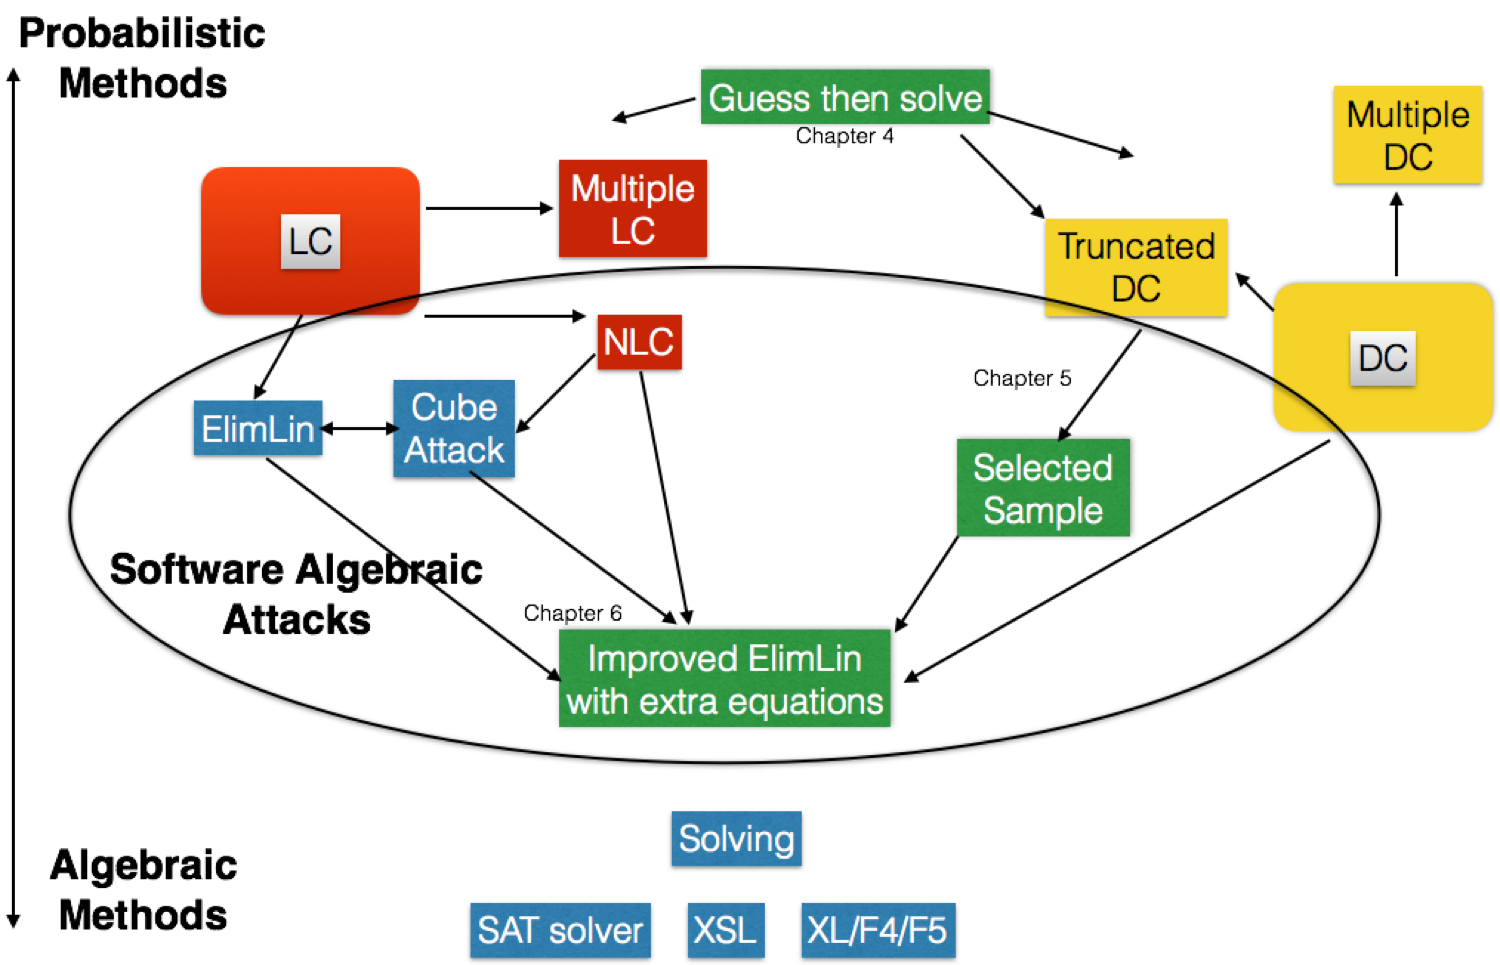
\includegraphics[width=130mm]{./pics/ch3general.png}	
	\caption[Classification of cryptanalysis methods and their connections]{Classification of cryptanalysis methods and their connections. Most of the existing literature considered algebraic cryptanalysis as an independent research area compare to probablisitic cryptanalysis methods such as differencial cryptanalysis (DC) and linear cryptanalysis (LC). We believe Algebraic Attacks has many connections. probablisitic method are often used together with Algebraic methods and in some attacks presented in this thesis they improved Algebraic Attacks performance by introduction new equations to the mathematic model and reduced solving complexity at the solving stage of Algebraic Attacks. Boxes colored in red are normally considered as LC. Yellow boxes are normally considered as DC methods. Green boxes are the parts included in this thesis and blue boxes are considered as specific solving methods}
	\label{fig:ch3general}
\end{figure}	

A link between ElimLin and linear cryptanalysis in Figure \ref{fig:ch3general} reflects the fact that both of these methods are looking for linear relations inside the cipher. However, a major difference between these two approaches is ElimLin looks for equations that work only for a particular set of P/C pairs\footnote{although some equations might exist for any P/C pairs}. Cube attack which was introduced by Dinur and Shamir in 2009 \cite{dinur2009cube} chooses a subset of 'public' input bits such that the sum of an output bit value is a linear combination of the key after a certain summation over a cube composed of plaintexts where a subset of bits varies. Cube attack can sometimes be linear and sometimes non-linear which can be seen as related to both ElimLin and Non-Linear Cryptanalysis (NLC) sometimes called Generalized Linear Cryptanalysis (GLC). In \cite{suvsil2016selection} the authors have studied how well-selected samples from cube attack can be used to improve the performance of ElimLin. Our research in general more or less accidentally identifies some of the equations which are also found in cube attacks and many more. One key focus is how different cryptanalysis techniques can be used to improve software algebraic attacks by adding more equations which makes that these attacks themselves will find yet more equations (amplification effect). 
In Chapter \ref{ch:SIMON} we show how well-selected samples following a truncated differential property can reduce the solving complexity of ElimLin and SAT solvers. Guess-then-solve method is a general cryptanalysis method which can be used in many attack scenarios. In Chapter \ref{ch:GOST} we will explore this type of attacks on Russian GOST cipher and show this method can be used to improve algebraic cryptanalysis with SAT solvers.

We conjecture that one can precompute additional linear equations that cannot be found by ElimLin, and provids those equations at the begining of solving step. This will speed up the entire solving process in software algebraic cryptanalysis. However, in this thesis we don't have a concrete example to proof our conjecture. Such work can be considered as future work for this thesis.

\section{Conclusion}

We have identified the source and the nature of cryptanalytic success of ElimLin. It comes from several phenomena: equations emerge by thresholds, they meet in the middle, they exhibit super-linear growth in some (crucial) cases, and we have discovered how to efficiently generate a lot more equations which ElimLin does not  typically find. We discovered that $J$ values can be quite large, but this does not translate into generating particularly large numbers of equations. This is somewhat contrary to intuition: 
for example equations which exist, even with a very small probability for every triple of encryptions, could grow up to as fast as $K^3$. This does not work as expected. 
In fact we have established an upper bound on such extra equations in the Known Plaintext Attack (KPA) scenario.  
In addition the Chosen Plaintext Attack(CPA) scenario remains a lot more promising. For example it can include cube attacks by Shamir and Dinur \cite{dinur2009cube} , some of which equations we have also already encountered in ElimLin runs and which opens a lot more hard optimization problems with regard to the basis of the cube. 

We have all the ingredients. However, designing a really optimal algebraic attack on a block cipher is not an easy task due to the large complexity of the equations we have discovered. 
We feel that each class of equations could be computed faster by a dedicated method, 
and we have already computed many substantially faster by our Polynomial Approximation method above. 
Moreover such methods could also compute several types of equations at once. 
Future research is needed on how ElimLin needs to be enhanced in practice and what kind trade-offs can be observed between the cost of computing various classes of equations we have already seen and others we have not yet fully integrated in ElimLin+ sort of attacks, as well as the cost of ElimLin itself. Due to sparsity and the specific character of various types of equations, it is not easy to know what is the most efficient method to compute all the equations or their linear equivalents, and it could be true that focusing on some fast growing 
and very sparse types/classes and ignoring some long equations which we already have will allow us to have an overall faster attack. 
If we had just one dominating type of equations with fast asymptotic growth, the analysis would be a lot easier. This is not what we observe for Simon and this could be different for another cipher. Similarly, if the statistic were flat maybe there would be little advantage focusing on some equations. 
We don't observe this either and we are in the case with several strong classes of equations. 


\chapter{Conclusion}
\label{chapterlabel4}

This thesis mainly focuses on improving algebraic cryptanalysis with software and solvers. Algebraic cryptanalysis is powerful as it requires small quantities of data, but in general the complexity grows quickly as the number of rounds increases. Many mitigations to improve runtimes are studied. 
We explored different types of optimization processes meant to make algebraic cryptanalysis problems transition from ``hard to solve" to ``easier to solve" by a software solver. We applied these optimizations to concrete ciphers and demonstrated the improvements. We aim to contribute to future government standards, such as Simon and other widely used ciphers including new releases of GOST.  We proposed several possible optimizations for algebraic cryptanalysis and experimentally demonstrated the attacks on GOST and Simon, which were submitted to ISO. We explore many powerful enhancements for algebraic attacks, and in one case we show a result which upper bounds can be obtained, and suggest a new method to predict the complexity of future attacks. 
We also propose an optimized attack for Bitcoin brain wallet attack.  

In Chapter 4, we introduced a new notion of contradiction immunity and SAT immunity, which converts a first stage in cryptanalysis of GOST to an optimization problem. Then we implemented a guess-then-solve attack with a well chosen set of guessed bits. This attack later directly improved the current best attack on GOST. Incidentally GOST was rejected by ISO at that time. 

In Chapters 5-6 we studied NSA block cipher Simon which was introduced in 2013 and submitted to ISO in 2015. 
We introduced a new method that uses well selected P/C pairs which follow a truncated differential property for algebraic cryptanalysis, and demonstrated the improvement on basic algebraic attacks on Simon with an extremely detailed study of what happens inside the attack and a serious improvement which generates more equations directly. Our work breaks 10/48 rounds of Simon64/128 with less than 10 P/C pairs.
We disagree when some researchers believe that Simon should not be studied by academics: 

\begin{quotation}
	``%`SIMON and SPECK should not even be reviewed by anyone in the community, 
	because it dignifies [the designs] and wastes the cycles – the brain cycles – of intelligent people, by going to look at a thing that is produced by a bad actor agency [(the NSA)]." \\ 
\rightline{{--- Jacob Appelbaum, FSE 2015 invited talk \phantom{This ble} }}
\end{quotation}

We propose an opposite view: it is important for the research community to study Simon because it is likely to become an important industry standard in the future. We published the first algebraic cryptanalysis work on Simon in 2014. Today, it is not the best attack. But it is important for the community to notice Simon's low multipicative complexity, low non-linearity and its low security against algebraic cryptanalysis which is also shown 
in Section \ref{Sec:ElimLinVsApprox}. 

In our research we spent a lot of time on contemplating what happens inside ElimLin algorithm. It contains a rich variety of attacks, for example, various generalizations of cube attacks not previously studied. 
ElimLin is a powerful tool for algebraic cryptanalysis, but with a fundamental limitation on computational complexity. When trying to solve larger number of rounds, the converted problems get much more bigger and ElimLin can not provide an answer within a short time. With a large number of experiments using ElimLin on Simon, we show that precise prediction for ElimLin is possible. We have made progress in both understanding better and extending/enhancing the ElimLin attack. Our discovery method 
of Section \ref{Sec:ElimLinVsApprox} suggests that the same equations can yet be computed a lot more efficiently. 

Finally, we also looked at the widely used cryptography application --  ECDSA in Bitcoin with the secp256k1 curve in Chapter 7. Elliptic curve problems themselves are hard algebraic cryptanalysis problems with complex polynomials and sometimes equations which follow the same topology as in a block cipher. Here nobody is yet able to 
propose advanced practical attacks. Another application we studied is Bitcoin. 
It was invented in 2008 and has grown rapidly since 2012, and it's one of the largest ECC practical applications in the world. We studied how some users manage their private keys and the security pitfalls related to this. Bitcoin uses a special elliptic curve secp256k1 which has not been widely used by any previous application, and in this thesis we provide a detailed benchmark of all the major implementations of this curve, and propose an optimized password cracking attack on Bitcoin brain wallets with a slightly unusual ECC  speed optimization. Our work together with other researchers work had made the Bitcoin community aware that brain wallets are extremely insecure.  
% This just dumps some pseudolatin in so you can see some text in place. 


\addcontentsline{toc}{chapter}{Appendices}

% The \appendix command resets the chapter counter, and changes the chapter numbering scheme to capital letters.
%\chapter{Appendices}
\appendix
\chapter{An Appendix About Stuff}
\label{appendixlabel1}
(stuff)

\chapter{Another Appendix About Things}
\label{appendixlabel2}
(things)

\chapter{Colophon}
\label{appendixlabel3}
\textit{This is a description of the tools you used to make your thesis. It helps people make future documents, reminds you, and looks good.}

\textit{(example)} This document was set in the Times Roman typeface using \LaTeX\ and Bib\TeX , composed with a text editor. 
 % description of document, e.g. type faces, TeX used, TeXmaker, packages and things used for figures. Like a computational details section.
% e.g. http://tex.stackexchange.com/questions/63468/what-is-best-way-to-mention-that-a-document-has-been-typeset-with-tex#63503

% Side note:
%http://tex.stackexchange.com/questions/1319/showcase-of-beautiful-typography-done-in-tex-friends 
% You could separate these out into different files if you have
%  particularly large appendices.

% This line manually adds the Bibliography to the table of contents.
% The fact that \include is the last thing before this ensures that it
% is on a clear page, and adding it like this means that it doesn't
% get a chapter or appendix number.
\addcontentsline{toc}{chapter}{Bibliography}

% Actually generates your bibliography.
\bibliography{PhD}

% All done. \o/
\end{document}
